\documentclass{fast-nuces-bs}
%\documentclass{article}
\usepackage[none]{hyphenat}   % disable word hyphenation
\usepackage{caption}
\captionsetup{font=small}
\usepackage{blindtext}
\usepackage{mathptmx}% Times Roman font
\usepackage[T1]{fontenc}
\usepackage{lipsum} 
\usepackage{sectsty}
\usepackage{tikz-uml}
\usepackage{titlesec}
\usepackage{tabularx}
\usepackage{array}
\usepackage{longtable}
\usepackage{placeins} % for \FloatBarrier

\usepackage{caption}
\usepackage{tabularx}
\usepackage{float}
\usepackage{graphicx}
\usepackage{caption}
\usepackage{float}
\usepackage{titlesec}
\usepackage{caption}
\usepackage{hyperref}
\usepackage{xcolor} % for colors

% ---------------- Packages ----------------
\usepackage{enumitem}   % for label=(\alph*) in enumerate
\usepackage{caption}    % better control of captions
\usepackage{float}      % for [H] placement of tables/figures
\usepackage{titlesec}   % control spacing around section headings

% ---------------- Formatting tweaks ----------------
\titlespacing*{\subsubsection}{0pt}{0.5em}{0.2em} % tighten spacing
\captionsetup[table]{skip=2pt} % reduce space between table & caption

% Reduce spacing after subsubsection headings
\titlespacing*{\subsubsection}{0pt}{0.5em}{0.2em}

% Reduce space around captions
\captionsetup[table]{skip=2pt}

% Information about the Thesis 
% -----------------------------------------------------------------------------
% (All are compulsory, do not delete any line other than author Information)
% For e.g., usually there are 3 students in a group, so leave authorone, 
% authortwo, and authorthree, and delete authorfour.
%%%%%%%%%%%%%%%%%%%%%%%%%%%%%%%%%%%%%%%%%%%%%%%%%%%%%%%%%%%%%%%%%%%%%%%%%%%%%%%
\department{Department of Computer Science}
\faculty{Computer Science}
\degreeyear{2026}
\degreemonth{June}
\degreename{Computer Science}
\campuscity{Islamabad}
\authorone{Inam Ullah Shaikh}{22i-0857}
\authortwo{Emaan Fatima}{22i-0869}
\authorthree{Aden Sial}{22i-1313}
\supervisor{Ms. Saira Qamar}
\sessionduration{2022-2026}
% \cosupervisor{Mr./ Ms./ Dr. Supervisor Name}
\deanname{Dr. Dean Computing}
\directorname{Dr. Director of the Campus}
\hodname{Dr. Head of Computer Science Department}
%\fypcoordinatorname{Name of FYP Coordinator}
\title{ForeSyte}
%%%%%%%%%%%%%%%%%%%%%%%%%%%%%%%%%%%%%%%%%%%%%%%%%%%%%%%%%%%%%%%%%%%%%%%%%%%%%%%

%%%%%%%%%%%%%%%%%%%%%%%%%%%%%%%%%%%%%%%%%%%%%%%%%%%%%%%%%%%%%%%%%%%%%%%%%%%%%%
% Former document starts below this
\begin{document}

%\begin{acknowledgements}
%	Your acknowledgments here
%\end{acknowledgements}

%\begin{abstract}
%Briefly state the (1) research problem, (2) methodology, (3) key results, and (4) conclusion. Generally, abstracts are between 150 and 200 words–roughly 10-15 sentences.
%\end{abstract}

\chapter{Introduction [AS PER SCOPE DOCUMENT]}
\label{sec:introduction}
The "Introduction" section sets the foundation for the entire report and should be carefully crafted to give the reader a clear understanding of the project’s scope, objectives, and context. Here’s what you can include:

Background:

Begin by providing background information on the broader topic or field your development project is related to.
Highlight any existing problems, gaps, or opportunities that led to the motivation for your project.
Include relevant references to previous research, development projects, or technologies. For example, you might want to cite studies or prior systems that failed to address the issues you're focusing on.


\section{Existing Solutions}

For the Existing Solutions section, students should research and describe various solutions, methods, or approaches that have been previously developed to solve the problem they are addressing. This section should include an overview of the different techniques, technologies, or models that are currently in use or have been applied in the past. Students should critically assess the strengths and weaknesses of each solution, highlighting any gaps or limitations that their project aims to address. Additionally, this section should show an understanding of the state-of-the-art in the field and provide context for why the proposed solution is necessary or an improvement over existing ones.


\begin{table}[H]
\centering
\caption{Comparison of Existing Solutions}
\begin{tabular}{|c|p{5cm}|p{5cm}|}
\hline
\textbf{System Name}   & \textbf{System Overview} & \textbf{System Limitations} \\ \hline
System 1               & Brief description of what System 1 does and its primary features. & Highlight the shortcomings or issues with System 1. \\ \hline
System 2               & Brief description of what System 2 does and its primary features. & Highlight the shortcomings or issues with System 2. \\ \hline
System 3               & Brief description of what System 3 does and its primary features. & Highlight the shortcomings or issues with System 3. \\ \hline
\end{tabular}
\label{tab:system_comparison}
\end{table}

\section{Problem Statement}
Academic dishonesty has become a significant concern in educational institutions worldwide. 
Studies indicate that approximately 61\% of university students have admitted to cheating during written examinations, 
while nearly 68\% confess to cheating at least once during their academic career \cite{bucciol2020cheating}. 
Traditional manual invigilation methods are often insufficient, as invigilators may unintentionally overlook suspicious activities, 
and reviewing long hours of CCTV/camera footage after exams is both time-consuming and ineffective.

To address these challenges, \textbf{ForeSyte} provides an AI-driven solution for automated examination monitoring. 
The system processes both real-time CCTV/camera streams and uploaded video footage, detecting suspicious activities such as 
phone usage, hand waving, bending over the desk, looking around, and standing up using advanced computer vision techniques.

The system focuses on seat-specific mapping, ensuring that every detected activity is linked to the correct student. 
It also ensures that the correct student ID is sitting on the assigned seat by using face recognition.  
In addition, \textbf{ForeSyte} incorporates an Invigilator Activity Monitoring module to:
\begin{itemize}
    \item Track invigilators' movements
    \item Detect prolonged idle periods
    \item Identify potential negligence
\end{itemize}
An admin dashboard provides real-time monitoring and automated report generation, enabling discipline committees to 
directly access timestamped violations instead of manually searching through hours of footage. 
By combining AI-powered surveillance with intelligent analytics, \textbf{ForeSyte} enhances exam security and aims to 
reduce academic dishonesty over time by providing actionable insights. Furthermore, as students become aware that their activities 
are continuously monitored and every suspicious action is captured with timestamped reports, the likelihood of cheating 
is expected to decrease significantly over repeated examination sessions

\begin{figure}[H]
    \centering
     \caption{Estimated reduction in cheating rates using ForeSyte AI-based surveillance system}
    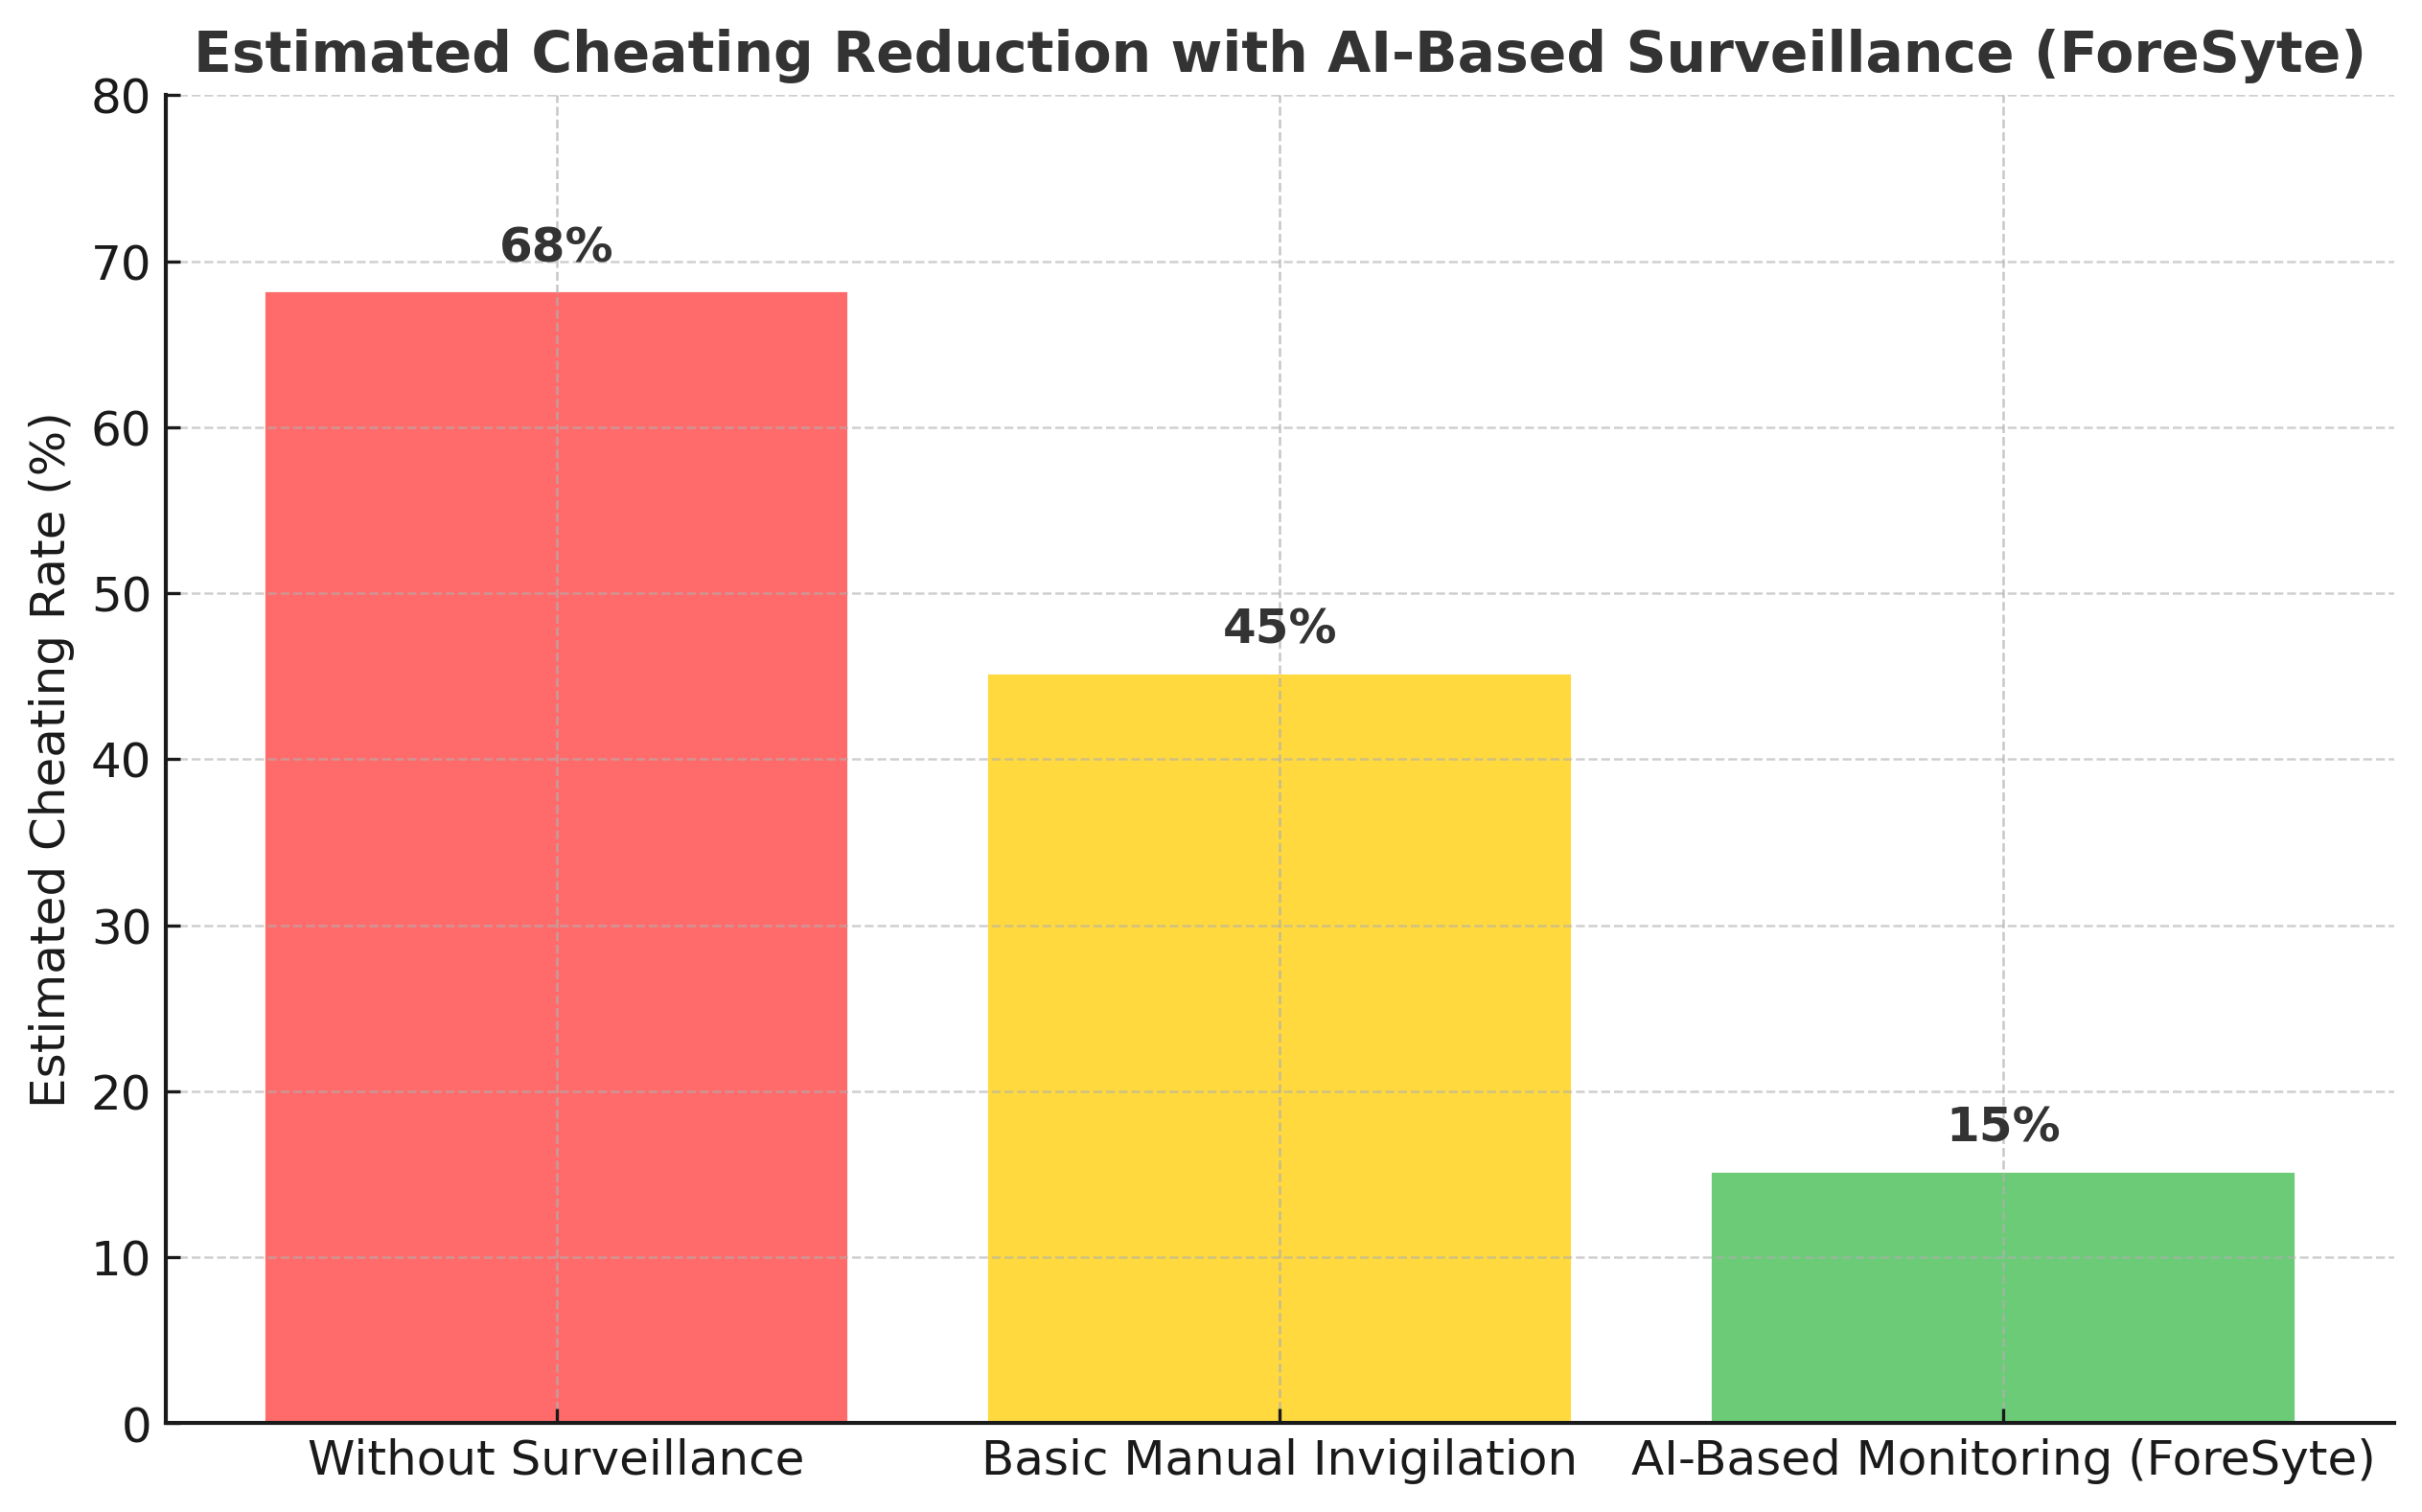
\includegraphics[width=0.8\linewidth]{sections/cheating_reduction_foreSyte.png}
    \label{fig:cheating_reduction}
\end{figure}

\begin{figure}[H]
    \centering
    \caption{Frequency of students who reported cheating during written examinations \cite{bucciol2020cheating}}
    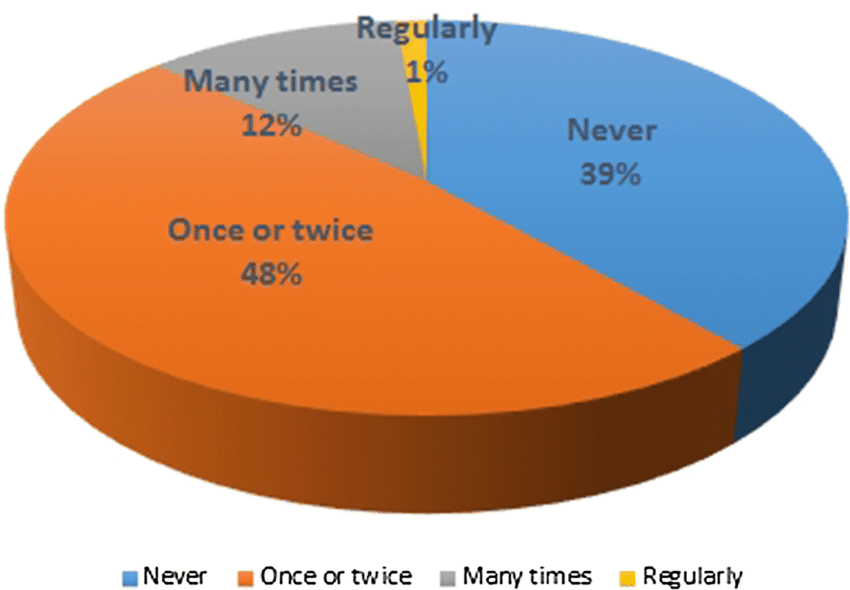
\includegraphics[width=0.7\linewidth]{sections/piechart.png}
    \label{fig:cheating_frequency}
\end{figure}
\FloatBarrier
\section{Scope}
The scope of the ForeSyte project includes developing an AI-powered exam surveillance 
system that enhances the integrity of examinations conducted in physical exam halls. 
Recent research highlights the importance of automated invigilation for maintaining 
academic integrity \cite{bucciol2020cheating, examIntegrity2021}. 

\begin{figure}[h]
    \centering
    \caption{Scope workflow of the ForeSyte system}
    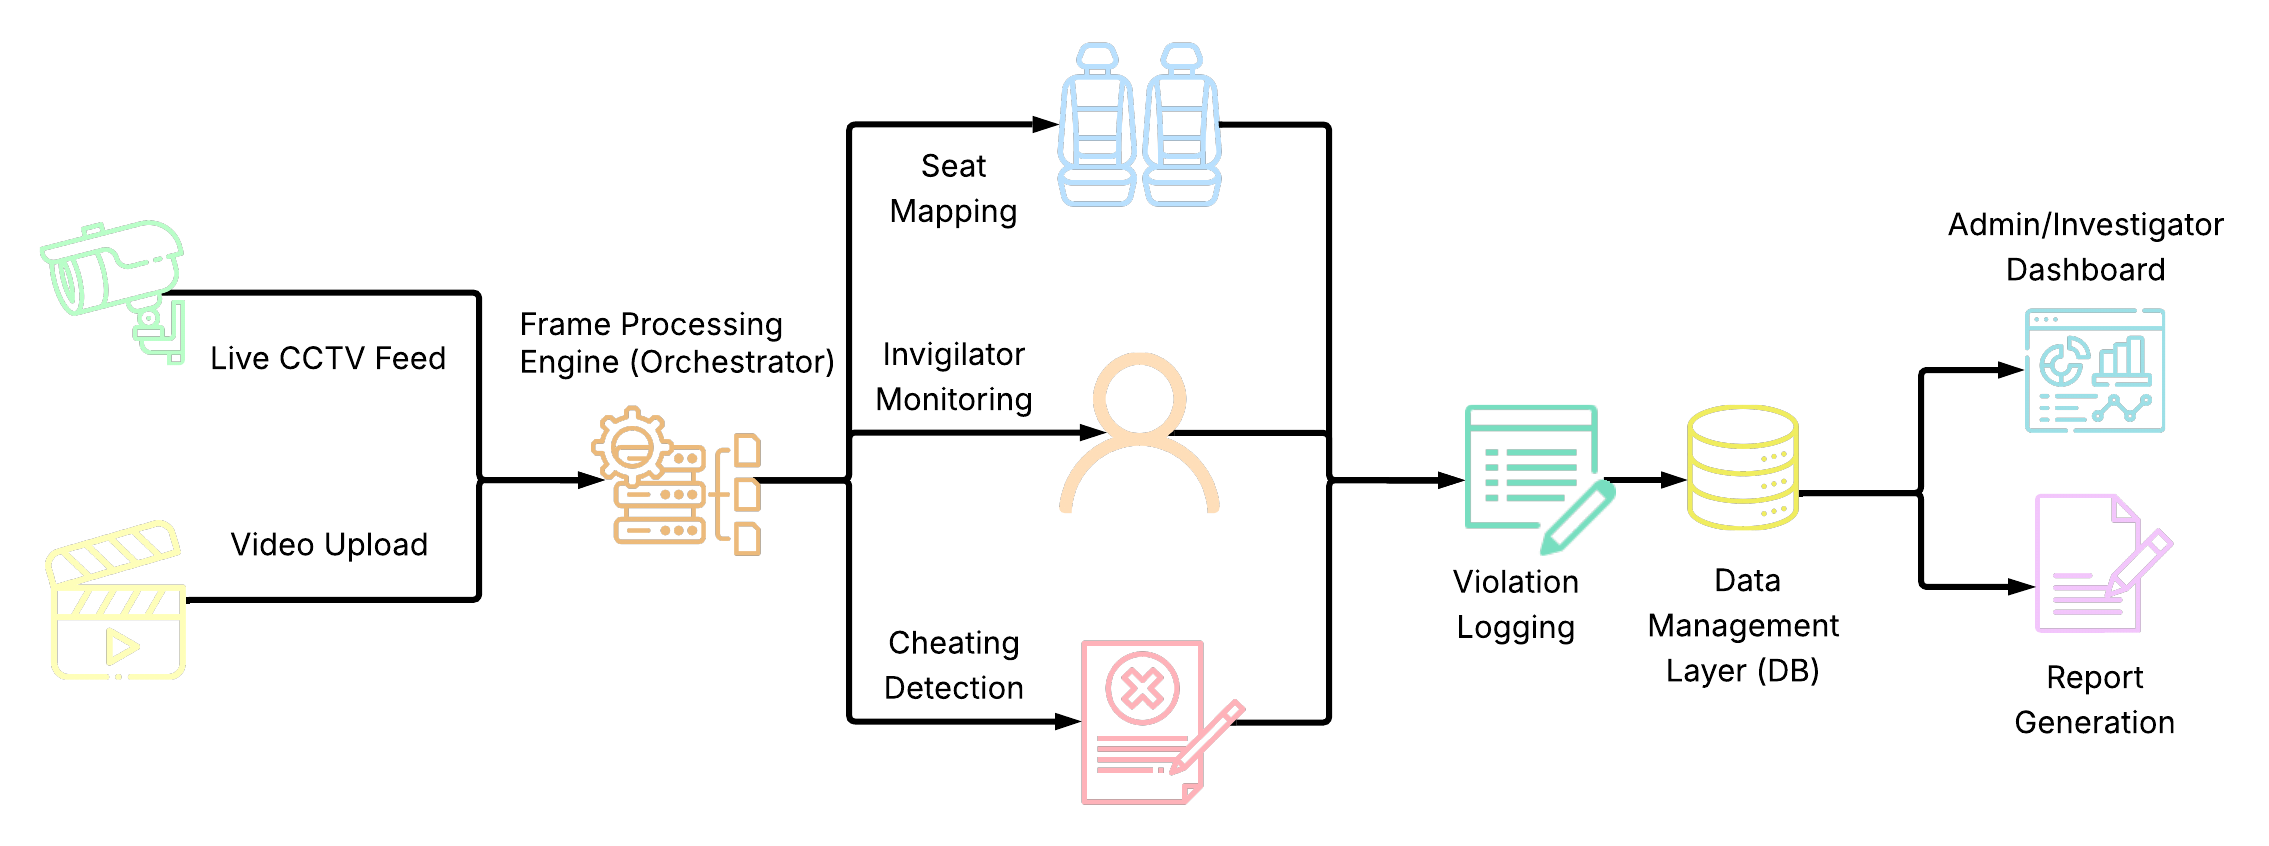
\includegraphics[width=0.9\textwidth]{sections/flowchart.png}
    \label{fig:flowchart}
\end{figure}

The system will process CCTV/camera footage, both live streams and uploaded recordings, to 
automatically detect and log suspicious activities such as unauthorized object usage and 
irregular gestures. It will also incorporate seating arrangement verification, ensuring that 
each detected activity is accurately linked to the correct student, and that the correct student ID 
is sitting in the assigned seat using face recognition, similar to approaches in modern proctoring systems \cite{masud2025cheating_detection, arumugam2025smart_invigilation}. 

The project further extends to monitoring invigilator activity within the exam hall, 
identifying negligence or prolonged absence from duty. Similar works on offline and 
intelligent monitoring systems support this approach \cite{holi2025iems, moyo2023openpose_exam_detection}. 
All detected events will be recorded with precise timestamps, seat numbers and room 
identifiers, enabling a structured and transparent record of violations.

An administrative dashboard will be developed to centralize monitoring and provide 
clear violation reports supported with visual evidence. This will reduce the need for 
institutions to manually review extensive CCTV/camera footage, offering instead a concise and 
accurate summary of flagged incidents. 

The system will be designed for real-time performance using optimized frame sampling 
and AI models capable of efficient video analysis. The project will be self-funded and 
developed entirely by our team. Related research also discusses the ethical implications of 
AI in exam supervision, highlighting fairness and privacy issues. 

The boundaries of this project are confined to creating a robust and intelligent surveillance 
solution that automates detection, verification, and reporting within physical exam 
environments, thereby ensuring greater fairness, efficiency, and accountability in academic assessments.
\section{Modules} 

The \textbf{ForeSyte} project is organized into several core modules, each responsible for specific functionalities required to ensure seamless, automated exam monitoring. 
The modules are divided into two main components: the \textit{ForeSyte Web Portal} for stakeholders and the \textit{Backend Service} that powers the AI-driven monitoring capabilities.

\subsection{ForeSyte Web Portal}
The \textbf{ForeSyte Web Portal} is a multi-user interface designed for administrators, discipline committee members, and university management. 
It provides centralized access to seating plans and violation reports, ensuring transparent and efficient management of examination activities.

\begin{enumerate}
    \setlength{\itemsep}{2pt}
    \item \textbf{Dashboard Visualization:} Displays real-time updates of suspicious activities, flagged violations, and invigilator presence across multiple exam halls using data from connected CCTV/camera systems.
    \item \textbf{Report Access:} Enables authorized users to view, manage, and download detailed violation reports containing timestamps, seat details and room information.
    \item \textbf{User Roles and Permissions:} Implements secure role-based access, where administrators manage seating plans, camera configurations, and exam schedules, while discipline committee members focus on reviewing reports and initiating actions.
    \item \textbf{Seating Plan Integration:} Links violations to student seating layouts and verifies correct student IDs using face recognition to ensure accurate identification of candidates involved in flagged incidents.
\end{enumerate}

\subsection{Backend Service}
The \textbf{Backend Service} powers the core intelligence of the ForeSyte system, managing video analysis, behavioral detection, invigilator monitoring, and reporting. 
This module processes video streams from CCTV/camera systems and uploaded exam footage to ensure accurate real-time and recorded exam monitoring.

\begin{enumerate}
    \setlength{\itemsep}{2pt}
    \item \textbf{Video Stream Processing:} Integrates with CCTV/camera systems and uploaded recordings, extracting frames for real-time detection of activities and events.
    \item \textbf{Cheating Detection Engine:} Uses advanced computer vision techniques to identify suspicious behaviors such as unauthorized object usage, irregular gestures, communication, and frequent seat movements \cite{bhatti2023smart, arumugam2025smart_invigilation}.
    \item \textbf{Face and Seat Verification:} Verifies student identities and ensures correct student ID is sitting on the assigned seat using face recognition, mapping detected activities to seating plans for accurate violation reporting.
    \item \textbf{Invigilator Monitoring:} Tracks invigilator's prolonged absences from assigned zones, and identifies potential negligence or unauthorized phone usage\cite{moyo2023openpose_exam_detection}.
    \item \textbf{Report Generation:} Compiles timestamped violation logs, including room details, seat numbers, and integrates them directly into the ForeSyte Web Portal for automated PDF/Excel report exports.
\end{enumerate}

\section{Work Division}
For each module and respective feature, responsibility is assigned to a team member.

\begin{table}[!h]
\centering
\begin{tabular}{|l|p{10cm}|}
\hline
\textbf{Name} & \textbf{Responsibility} \\ \hline

Inam Ullah Shaikh & 
\begin{itemize}
    \item Frontend Development
    \item Model Training
    \item Documentation
    \item Deployment
    \item Backend Integration
\end{itemize} \\ \hline

Emaan Fatima & 
\begin{itemize}
    \item Backend Development
    \item Model Research
    \item Model Training
    \item Documentation
    \item Deployment
\end{itemize} \\ \hline

Aden Sial & 
\begin{itemize}
    \item Data Collection
    \item Model Training
    \item Model Research
    \item Documentation
    \item Deployment
\end{itemize} \\ \hline

\end{tabular}
\caption{Work Division among Team Members}
\end{table}

\newpage


\chapter{Project Requirements [AS PER FYP1 MID REPORT]}
This chapter describes the functional and non-functional requirements of the project. 
\section{Use-cases}
The Table 2.1 lists down all the possible use cases for our project. 
Note that login, sign up and feedback pages are not included in these use cases.
% ---------- Summary Table ----------
\begin{table}[htbp]
\caption{Summary of Use Cases for ForeSyte}
\centering
\begin{tabular}{|c|p{4cm}|p{8cm}|}
\hline
\textbf{Usecase ID} & \textbf{Use Case Name} & \textbf{Description} \\ \hline
UC-01 & View \& Manage Reports/Dashboard & Authorized users view and manage reports of student and invigilator activity. \\ \hline
UC-02 & Manage User Profiles & System administrator manages accounts and roles of all users. \\ \hline
UC-03 & Generate Detection Reports & System generates timestamped reports of detected cheating or negligence. \\ \hline
UC-04 & Verify Student Identity \& Seat Mapping & System verifies student identity using face recognition and assigned seats. \\ \hline
UC-05 & Monitor Invigilator Activity & System monitors invigilators for negligence, absence, or unauthorized actions. \\ \hline
UC-06 & Monitor Student Behaviour & System monitors student actions to detect cheating attempts. \\ \hline
UC-07 & Process Exam Footage (Live/Recorded) & System processes live and recorded video streams to detect activities. \\ \hline
\end{tabular}
\end{table}
\vspace{0.5cm} % <-- add some vertical space

% Text outside tables
  Below, you can find the detailed use case description for each use case.
\clearpage

% ---------- UC-01 ----------
\subsubsection*{2.1.1\quad UC-01}

\begin{longtable}{|p{5cm}|p{10cm}|}
\caption{Use Case 1: View \& Manage Reports/Dashboard} \label{uc1} \\

\hline
\textbf{Use Case Detail} & \textbf{Description} \\ \hline
Use Case ID & UC-01 \\ \hline
Use Case Name & View \& Manage Reports/Dashboard \\ \hline
Scope & ForeSyte Web Portal \\ \hline
Level & User Goal \\ \hline
Brief Description & Users view, filter, and manage real-time dashboards and past reports. \\ \hline
Actor(s) Involved & System Administrator, Investigator, Discipline Committee \\ \hline
Stakeholders & • Discipline Committee: Reviews violation data \newline • Admins: Configure reports \\ \hline
Pre-conditions & Reports and logs already generated by detection system. \\ \hline
Post-conditions & Users access detailed dashboards with downloadable reports. \\ \hline
Main Success Scenario & 
1. Actor logs into the ForeSyte Web Portal successfully. \newline
2. Actor navigates to the Reports/Dashboard section from the main menu. \newline
3. System retrieves all available violation reports from the database. \newline
4. System displays a dashboard with filters (e.g., by student ID, seat number, violation type, or timestamp). \newline
5. Actor applies filters to refine the report view. \newline
6. System dynamically updates the dashboard according to the selected filters. \newline
7. Actor selects a specific report for detailed view. \newline
8. System displays complete details of the selected report (student, invigilator, time, violation evidence). \newline
9. Actor chooses the option to download or export the report. \newline
10. System generates the report in the selected format (PDF/Excel) and confirms successful export. \\ \hline

Special Requirements & Role-based access, secure data visualization \\ \hline

\end{longtable}

\clearpage

% ---------- UC-02 ----------
\subsubsection*{2.1.2\quad UC-02}
\begin{longtable}{|p{5cm}|p{10cm}|}
\caption{Use Case 2: Manage User Profiles} \label{uc1} \\
\hline

\textbf{Use Case Detail} & \textbf{Description} \\ \hline
Use Case ID & UC-02 \\ \hline
Use Case Name & Manage User Profiles \\ \hline
Scope & ForeSyte Web Portal \\ \hline
Level & User Goal \\ \hline
Brief Description & System administrator manages user accounts, roles, and permissions. \\ \hline
Actor(s) Involved & System Administrator \\ \hline
Stakeholders & • Admins: Maintain structured access \\ \hline
Pre-conditions & Admin is authenticated. \\ \hline
Post-conditions & User accounts created, modified, or deleted. \\ \hline
Main Success Scenario & 
1. Admin logs into the ForeSyte Web Portal. \newline
2. Admin navigates to the User Management module. \newline
3. System displays the list of existing users with their roles. \newline
4. Admin selects an action (add, edit, or delete a user). \newline
5. If adding: Admin enters new user details including username, role, and credentials. \newline
6. If editing: Admin updates user details or permissions. \newline
7. If deleting: Admin selects a user and confirms deletion. \newline
8. System validates the request and updates the database accordingly. \newline
9. System confirms success with a message (user added/updated/deleted). \newline
10. Admin logs out or continues with further management tasks. \\ \hline

Special Requirements & Secure password policies, role-based restrictions \\ \hline

\end{longtable}

\clearpage

% ---------- UC-03 ----------
\subsubsection*{2.1.3\quad UC-03}
\begin{longtable}{|p{5cm}|p{10cm}|}
\caption{Use Case 3: Generate Detection Reports}\label{uc1} \\
\hline
\textbf{Use Case Detail} & \textbf{Description} \\ \hline
Use Case ID & UC-03 \\ \hline
Use Case Name & Generate Detection Reports \\ \hline
Scope & Backend Service + Web Portal \\ \hline
Level & User Goal \\ \hline
Brief Description & System generates timestamped detection reports of suspicious activity. \\ \hline
Actor(s) Involved & Investigator, Discipline Committee \\ \hline
Stakeholders & • Discipline Committee: Reviews reports \newline • University Management \\ \hline
Pre-conditions & Detection system has analyzed video footage. \\ \hline
Post-conditions & Report generated and stored in database. \\ \hline
Main Success Scenario & 
1. AI detection engine processes exam footage. \newline
2. System identifies suspicious activity (e.g., phone usage, looking around, invigilator negligence). \newline
3. System logs details including timestamp, seat number, room, and involved actor. \newline
4. System compiles the violation data into a structured report format. \newline
5. Investigator accesses the Web Portal and navigates to the Reports section. \newline
6. System displays the list of generated reports. \newline
7. Investigator selects a specific report for review. \newline
8. System displays detailed evidence including video snippets or screenshots. \newline
9. Investigator verifies and approves the report for further review. \newline
10. Report is stored in the system and available for export (PDF/Excel). \\ \hline

Special Requirements & Reports exportable to PDF/Excel \\ \hline

\end{longtable}

\clearpage

% ---------- UC-04 ----------
\subsubsection*{2.1.4\quad UC-04}
\begin{longtable}{|p{5cm}|p{10cm}|}
\caption{Use Case 4: Verify Student Identity \& Seat Mapping}\label{uc1} \\
\hline
\textbf{Use Case Detail} & \textbf{Description} \\ \hline
Use Case ID & UC-04 \\ \hline
Use Case Name & Verify Student Identity \& Seat Mapping \\ \hline
Scope & Backend Service \\ \hline
Level & User Goal \\ \hline
Brief Description & System verifies student identity using face recognition and seat mapping. \\ \hline
Actor(s) Involved & Student, Invigilator \\ \hline
Stakeholders & • University Management \\ \hline
Pre-conditions & Seating plan and student ID data available. \\ \hline
Post-conditions & Student identity verified and mapped. \\ \hline
Main Success Scenario & 
1. Exam seating plan is uploaded into the system. \newline
2. Student enters the exam hall and sits on the assigned seat. \newline
3. System activates facial recognition through CCTV or camera feed. \newline
4. System captures the student’s face and compares it with pre-stored student records. \newline
5. System checks whether the student is seated in the correct assigned seat. \newline
6. If the identity matches, the system confirms successful verification. \newline
7. If there is a mismatch, the system flags the seat for manual review by the examiner. \newline
8. System logs the verification results along with seat ID and student ID. \newline
9. Verified data is linked to subsequent activity monitoring and reports. \\ \hline
Special Requirements & Reliable face recognition with low error rate \\ \hline


\end{longtable}

\clearpage

% ---------- UC-05 ----------
\subsubsection*{2.1.5\quad UC-05}
\begin{longtable}{|p{5cm}|p{10cm}|}
\caption{Use Case 5: Monitor Invigilator Activity}\label{uc1} \\
\hline
\textbf{Use Case Detail} & \textbf{Description} \\ \hline
Use Case ID & UC-05 \\ \hline
Use Case Name & Monitor Invigilator Activity \\ \hline
Scope & Backend Service \\ \hline
Level & User Goal \\ \hline
Brief Description & System tracks invigilators for negligence, absence, or unauthorized actions. \\ \hline
Actor(s) Involved & Invigilator, Discipline Committee \\ \hline
Stakeholders & • University Management \\ \hline
Pre-conditions & Cameras active and invigilator zones defined. \\ \hline
Post-conditions & Invigilator activity log generated. \\ \hline
Main Success Scenario & 
1. Surveillance cameras start recording invigilator activity. \newline
2. System tracks invigilator’s presence across different zones of the exam hall. \newline
3. AI analyzes the video feed to detect movement or prolonged inactivity. \newline
4. If invigilator leaves their zone for too long, the system flags negligence. \newline
5. If invigilator is using unauthorized devices (e.g., phone), system captures it. \newline
6. System logs the timestamp, location, and detected action. \newline
7. Discipline Committee accesses the dashboard to view invigilator logs. \newline
8. System displays flagged negligence cases in the report. \newline
9. Committee reviews and validates the report. \newline
10. Finalized invigilator activity log is stored and exported if needed. \\ \hline

Special Requirements & Accurate zone mapping \\ \hline

\end{longtable}

\clearpage

% ---------- UC-06 ----------
\subsubsection*{2.1.6\quad UC-06}
\begin{longtable}{|p{5cm}|p{10cm}|}
\caption{Use Case 6: Monitor Student Behaviour}\label{uc1} \\
\hline
\textbf{Use Case Detail} & \textbf{Description} \\ \hline
Use Case ID & UC-06 \\ \hline
Use Case Name & Monitor Student Behaviour \\ \hline
Scope & Backend Service \\ \hline
Level & User Goal \\ \hline
Brief Description & Detects cheating behaviors (phone use, gestures, looking around). \\ \hline
Actor(s) Involved & Student, Investigator \\ \hline
Stakeholders & • Discipline Committee \newline • University Management \\ \hline
Pre-conditions & Camera feed and detection models active. \\ \hline
Post-conditions & Violations logged with timestamps. \\ \hline
Main Success Scenario & 
1. Exam begins and surveillance cameras monitor all students. \newline
2. AI detection model continuously analyzes student actions. \newline
3. System identifies suspicious behavior such as phone use, hand gestures, or looking around repeatedly. \newline
4. When detected, system flags the behavior as a potential violation. \newline
5. System records timestamp, seat ID, and video evidence. \newline
6. Investigator accesses the dashboard to review logged violations. \newline
7. System displays detailed violation logs with associated video frames. \newline
8. Investigator examines the evidence for each flagged action. \newline
9. Investigator confirms or dismisses the violation. \newline
10. Validated violations are added to the final exam report. \\ \hline
Special Requirements & Must differentiate normal vs cheating actions \\ \hline

\end{longtable}

\clearpage

% ---------- UC-07 ----------
\subsubsection*{2.1.7\quad UC-07}
\begin{longtable}{|p{5cm}|p{10cm}|}
\caption{Use Case 7: Process Exam Footage (Live/Recorded)}\label{uc1} \\
\hline
\textbf{Use Case Detail} & \textbf{Description} \\ \hline
Use Case ID & UC-07 \\ \hline
Use Case Name & Process Exam Footage (Live/Recorded) \\ \hline
Scope & Backend Service \\ \hline
Level & User Goal \\ \hline
Brief Description & System processes live and recorded exam video footage for analysis. \\ \hline
Actor(s) Involved & System Administrator, Investigator \\ \hline
Stakeholders & • University Management \\ \hline
Pre-conditions & Camera streams or uploaded recordings available. \\ \hline
Post-conditions & Footage analyzed and results stored. \\ \hline
Main Success Scenario & 
1. System connects to live CCTV cameras or receives uploaded exam recordings. \newline
2. System validates video input and prepares it for analysis. \newline
3. AI engine processes video frames in real time or batch mode. \newline
4. System identifies and logs suspicious student or invigilator behavior. \newline
5. System maps detected activity to the correct student seat. \newline
6. All activities are logged with timestamps and stored in the database. \newline
7. Investigator accesses the Reports module. \newline
8. System displays results of processed footage (violations, seat mapping). \newline
9. Investigator reviews the logged activities and evidence. \newline
10. Reports are finalized and exported in required format. \\ \hline

Special Requirements & Efficient processing, storage optimization \\ \hline

\end{longtable}
\clearpage
% ---------- Use Case Diagram ----------
\subsection*{2.1.8\quad Use Case Diagram of ForeSyte}

The Figure \textcolor{blue}{\ref{fig:usecase}} highlights the use case diagram of the entire ForeSyte Web Application.


\begin{figure}[htbp]
    \centering
    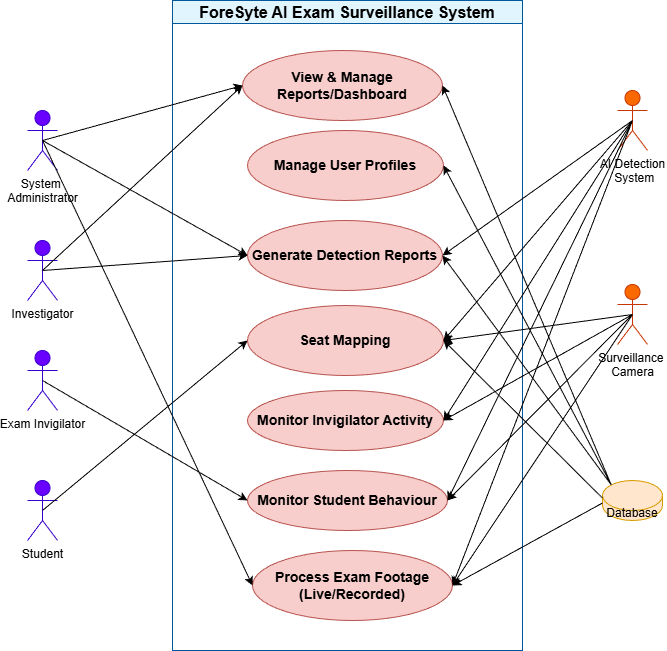
\includegraphics[width=\textwidth]{sections/usecase.png}
    \caption{ForeSyte Use Case Diagram}
    \label{fig:usecase}
\end{figure}

\section{Functional Requirements}
This section describes the functional requirements of ForeSyte arranged in a use case-based organizational method.

% ---------- UC-01 ----------
\subsubsection*{2.2.1\quad UC-01 Functional Requirement}
\vspace{-0.5em}
\begin{table}[H]
\caption{Functional Requirements for UC-01}
\centering
\begin{tabular}{|c|p{11cm}|}
\hline
\textbf{Functional Requirement ID} & \textbf{Description} \\ \hline
FR-01 & The system shall allow authorized users to log in and access the Reports/Dashboard module. \\ \hline
FR-02 & The system shall display real-time and historical reports of student and invigilator activity. \\ \hline
FR-03 & The system shall provide filtering options (by student ID, seat number, violation type, timestamp). \\ \hline
FR-04 & The system shall allow exporting reports in PDF and Excel formats. \\ \hline
FR-05 & The system shall enforce role-based access to reports. \\ \hline
\end{tabular}
\end{table}

% ---------- UC-02 ----------
\subsubsection*{2.2.2\quad UC-02 Functional Requirement}
\vspace{-0.5em}
\begin{table}[H]
\caption{Functional Requirements for UC-02}
\centering
\begin{tabular}{|c|p{11cm}|}
\hline
\textbf{Functional Requirement ID} & \textbf{Description} \\ \hline
FR-06 & The system shall allow the administrator to add new user accounts with role assignments. \\ \hline
FR-07 & The system shall allow editing of existing user details and permissions. \\ \hline
FR-08 & The system shall allow deleting user accounts securely. \\ \hline
FR-09 & The system shall validate inputs (username, password, role) before saving. \\ \hline
FR-10 & The system shall enforce strong password and security policies. \\ \hline
\end{tabular}
\end{table}

% ---------- UC-03 ----------
\subsubsection*{2.2.3\quad UC-03 Functional Requirement}
\vspace{-0.5em}
\begin{table}[H]
\caption{Functional Requirements for UC-03}
\centering
\begin{tabular}{|c|p{11cm}|}
\hline
\textbf{Functional Requirement ID} & \textbf{Description} \\ \hline
FR-11 & The system shall automatically generate detection reports when violations are flagged. \\ \hline
FR-12 & The system shall include timestamps, seat numbers, and violation type in reports. \\ \hline
FR-13 & The system shall store generated reports in a database. \\ \hline
FR-14 & The system shall allow investigators to review and approve reports. \\ \hline
FR-15 & The system shall allow reports to be exported in PDF/Excel format. \\ \hline
\end{tabular}
\end{table}

% ---------- UC-04 ----------
\subsubsection*{2.2.4\quad UC-04 Functional Requirement}
\vspace{-0.5em}
\begin{table}[H]
\caption{Functional Requirements for UC-04}
\centering
\begin{tabular}{|c|p{11cm}|}
\hline
\textbf{Functional Requirement ID} & \textbf{Description} \\ \hline
FR-16 & The system shall verify student identity using face recognition. \\ \hline
FR-17 & The system shall cross-check student identity against pre-stored records. \\ \hline
FR-18 & The system shall map verified students to their assigned seat numbers. \\ \hline
FR-19 & The system shall log verification results (student ID, seat ID, verification status). \\ \hline
FR-20 & The system shall flag mismatches for manual review. \\ \hline
\end{tabular}
\end{table}

% ---------- UC-05 ----------
\subsubsection*{2.2.5\quad UC-05 Functional Requirement}
\vspace{-0.5em}
\begin{table}[H]
\caption{Functional Requirements for UC-05}
\centering
\begin{tabular}{|c|p{11cm}|}
\hline
\textbf{Functional Requirement ID} & \textbf{Description} \\ \hline
FR-21 & The system shall monitor invigilators during exam sessions. \\ \hline
FR-22 & The system shall track invigilator presence in defined zones. \\ \hline
FR-23 & The system shall detect unauthorized activities (e.g., phone use). \\ \hline
FR-24 & The system shall log negligence events with timestamp and location. \\ \hline
FR-25 & The system shall provide invigilator activity logs to the Discipline Committee. \\ \hline
\end{tabular}
\end{table}

% ---------- UC-06 ----------
\subsubsection*{2.2.6\quad UC-06 Functional Requirement}
\vspace{-0.5em}
\begin{table}[H]
\caption{Functional Requirements for UC-06}
\centering
\begin{tabular}{|c|p{11cm}|}
\hline
\textbf{Functional Requirement ID} & \textbf{Description} \\ \hline
FR-26 & The system shall analyze student actions in real time. \\ \hline
FR-27 & The system shall detect suspicious behaviors (phone use, hand gestures, looking around). \\ \hline
FR-28 & The system shall differentiate between normal and abnormal behaviors. \\ \hline
FR-29 & The system shall log violations with seat ID, timestamp, and video snippet. \\ \hline
FR-30 & The system shall allow investigators to review and confirm logged violations. \\ \hline
\end{tabular}
\end{table}

% ---------- UC-07 ----------
\subsubsection*{2.2.7\quad UC-07 Functional Requirement}
\vspace{-0.5em}
\begin{table}[H]
\caption{Functional Requirements for UC-07}
\centering
\begin{tabular}{|c|p{11cm}|}
\hline
\textbf{Functional Requirement ID} & \textbf{Description} \\ \hline
FR-31 & The system shall process both live CCTV feeds and uploaded recordings. \\ \hline
FR-32 & The system shall analyze frames using AI detection models. \\ \hline
FR-33 & The system shall log activities with timestamps and seat IDs. \\ \hline
FR-34 & The system shall store processed results in the database. \\ \hline
FR-35 & The system shall make analyzed results available in the Reports module. \\ \hline
\end{tabular}
\end{table}

% ---------- General ----------
\subsubsection*{2.2.8\quad General Functional Requirements}
\vspace{-0.5em}
\begin{table}[H]
\caption{General Functional Requirements}
\centering
\begin{tabular}{|c|p{11cm}|}
\hline
\textbf{Functional Requirement ID} & \textbf{Description} \\ \hline
FR-36 & The system shall ensure processing of violations and reports within 20 seconds. \\ \hline
FR-37 & The system shall implement secure storage and encryption of student/exam data. \\ \hline
FR-38 & The system shall allow a responsive web interface for investigators and administrators. \\ \hline
FR-39 & The system shall maintain audit logs for all activities. \\ \hline
FR-40 & The system shall support scalability for multiple exam halls simultaneously. \\ \hline
\end{tabular}
\end{table}
\subsection*{2.2.9\quad Module 1: ForeSyte Web Portal}
Following are the requirements for Module 1 (ForeSyte Web Portal):

\begin{enumerate}
    \item \textbf{Dashboard Visualization}
    \begin{enumerate}[label=(\alph*)]
        \item FR-01: The system shall allow authorized users to log in and access the Reports/Dashboard module.
        \item FR-02: The system shall display real-time and historical reports of student and invigilator activity.
        \item FR-03: The system shall provide filtering options (by student ID, seat number, violation type, timestamp).
        \item FR-04: The system shall allow exporting reports in PDF and Excel formats.
        \item FR-05: The system shall enforce role-based access to reports.
    \end{enumerate}

    \item \textbf{Report Access}
    \begin{enumerate}[label=(\alph*)]
        \item FR-11: The system shall automatically generate detection reports when violations are flagged.
        \item FR-12: The system shall include timestamps, seat numbers, and violation type in reports.
        \item FR-13: The system shall store generated reports in a database.
        \item FR-14: The system shall allow investigators to review and approve reports.
        \item FR-15: The system shall allow reports to be exported in PDF/Excel format.
    \end{enumerate}

    \item \textbf{User Roles and Permissions}
    \begin{enumerate}[label=(\alph*)]
        \item FR-06: The system shall allow the administrator to add new user accounts with role assignments.
        \item FR-07: The system shall allow editing of existing user details and permissions.
        \item FR-08: The system shall allow deleting user accounts securely.
        \item FR-09: The system shall validate inputs (username, password, role) before saving.
        \item FR-10: The system shall enforce strong password and security policies.
    \end{enumerate}
\end{enumerate}


\subsection*{2.2.10\quad Module 2: Backend Service}
Following are the requirements for Module 2 (Backend Service):

\begin{enumerate}
    \item \textbf{Video Stream Processing}
    \begin{enumerate}[label=(\alph*)]
        \item FR-31: The system shall process both live CCTV feeds and uploaded recordings.
        \item FR-32: The system shall analyze frames using AI detection models.
        \item FR-33: The system shall log activities with timestamps and seat IDs.
        \item FR-34: The system shall store processed results in the database.
        \item FR-35: The system shall make analyzed results available in the Reports module.
    \end{enumerate}

    \item \textbf{Cheating Detection Engine}
    \begin{enumerate}[label=(\alph*)]
        \item FR-26: The system shall analyze student actions in real time.
        \item FR-27: The system shall detect suspicious behaviors (phone use, hand gestures, looking around).
        \item FR-28: The system shall differentiate between normal and abnormal behaviors.
        \item FR-29: The system shall log violations with seat ID, timestamp, and video snippet.
        \item FR-30: The system shall allow investigators to review and confirm logged violations.
    \end{enumerate}

    \item \textbf{Face and Seat Verification}
    \begin{enumerate}[label=(\alph*)]
        \item FR-16: The system shall verify student identity using face recognition.
        \item FR-17: The system shall cross-check student identity against pre-stored records.
        \item FR-18: The system shall map verified students to their assigned seat numbers.
        \item FR-19: The system shall log verification results (student ID, seat ID, verification status).
        \item FR-20: The system shall flag mismatches for manual review.
    \end{enumerate}

    \item \textbf{Invigilator Monitoring}
    \begin{enumerate}[label=(\alph*)]
        \item FR-21: The system shall monitor invigilators during exam sessions.
        \item FR-22: The system shall track invigilator presence in defined zones.
        \item FR-23: The system shall detect unauthorized activities (e.g., phone use).
        \item FR-24: The system shall log negligence events with timestamp and location.
        \item FR-25: The system shall provide invigilator activity logs to the Discipline Committee.
    \end{enumerate}

    \item \textbf{Report Generation and Security}
    \begin{enumerate}[label=(\alph*)]
        \item FR-36: The system shall ensure processing of violations and reports within 20 seconds.
        \item FR-37: The system shall implement secure storage and encryption of student/exam data.
        \item FR-38: The system shall allow a responsive web interface for investigators and administrators.
        \item FR-39: The system shall maintain audit logs for all activities.
        \item FR-40: The system shall support scalability for multiple exam halls simultaneously.
    \end{enumerate}
\end{enumerate}


\section{Non-Functional Requirements}
This section specifies the non-functional requirements of the ForeSyte system. These requirements are practical, measurable, and verifiable to ensure the system can be realistically implemented in an academic setting. 

\subsection{Reliability}
\begin{itemize}
    \item REL-1: The system shall achieve at least 95\% uptime during scheduled exam sessions.  
    \item REL-2: In case of camera or feed failure, the system shall log the event and notify the administrator within 1 minute.  
    \item REL-3: The system shall store video footage and violation data redundantly to prevent data loss.  
\end{itemize}

\subsection{Usability}
\begin{itemize}
    \item USE-1: An administrator shall be able to generate a violation report in no more than 3 interactions.  
    \item USE-2: New users (administrators or investigators) shall be able to learn the core functions of the system with less than 2 hours of training.  
    \item USE-3: The dashboard shall present violation summaries in a clear tabular format with filters.
\end{itemize}

\subsection{Performance}
\begin{itemize}
    \item PER-1: The system shall process live camera feeds with a maximum latency of 10 seconds.  
    \item PER-2: The cheating detection engine shall analyze at least 20 frames per second per camera feed.  
    \item PER-3: Violation reports shall be generated within 20 minutes of the end of an exam session.  
\end{itemize}

\subsection{Security}
\begin{itemize}
    \item SEC-1: Only authenticated users shall access the system dashboard.  
    \item SEC-2: User access shall be role-based (administrator, investigator).  
    \item SEC-3: All access attempts shall be logged for audit purposes.  
\end{itemize}

\subsection{Maintainability}
\begin{itemize}
    \item MAI-1: The system shall follow a modular architecture so that detection models can be updated independently.  
    \item MAI-2: Minor bugs shall be diagnosable and fixable within 48 hours.  
    \item MAI-3: The documentation shall describe system modules, and troubleshooting in detail for developers.  
\end{itemize}
\clearpage




\chapter{System Overview [AS PER FYP1 MID REPORT]}

\textbf{ForeSyte} AI Exam Surveillance System is an intelligent monitoring solution designed to enhance the integrity of in-person examinations by automating student and invigilator monitoring. The system integrates CCTV cameras, computer vision, and deep learning models to detect suspicious student behaviors such as phone usage, frequent seat movements, or unauthorized communication, while also tracking invigilator activities to ensure accountability. Each activity is mapped to seating plans to ensure accurate identification of students. Detected events are logged as timestamped violations, which are compiled into structured reports accessible through an administrative dashboard. Administrators manage user profiles, seating plans, and exam sessions, while disciplinary investigators utilize the violation reports to review cases and make informed decisions. The system follows a modular architecture consisting of two primary components: the ForeSyte Web Portal, a multi-user web interface for dashboard visualization and report management, and the Backend Service, the core AI engine handling video stream processing, cheating detection, seat mapping, and automated report generation. This architectural design ensures separation of concerns, scalability, and maintainability while providing seamless integration between the user interface and the underlying AI processing capabilities.

\section{Architectural Design}

The ForeSyte AI Exam Surveillance System is designed using a modular architecture to ensure scalability, maintainability, and clear separation of concerns. At a high level, the system is divided into front-end modules, back-end modules, and supporting external systems. Each module plays a distinct role but collaborates with others to achieve the overall goal of automated, AI-powered exam monitoring.

The architecture follows a \textbf{two-tier client-server architecture} with \textbf{layered components}, implementing a \textbf{RESTful API} design pattern. The front-end (presentation tier) handles user input, report visualization, and dashboard interactions through a React-based single-page application. The back-end (application tier) processes video streams, performs AI-based detection and analysis, and manages business logic through FastAPI routes. The data management layer (data tier) ensures persistence and retrieval of information using PostgreSQL for relational data and MongoDB for high-velocity event logs. This decomposition ensures that the AI detection logic, data storage, and user interfaces remain loosely coupled and independently upgradable.

\subsection{Box and Line Diagram (Initial Design Stage)}
In the initial design stage, a simple box and line diagram is used to represent the main system components and their interactions. This diagram provides a high-level overview of how the core modules connect, without detailing the internal architecture or data flow.

\begin{figure}[H]
    \centering
    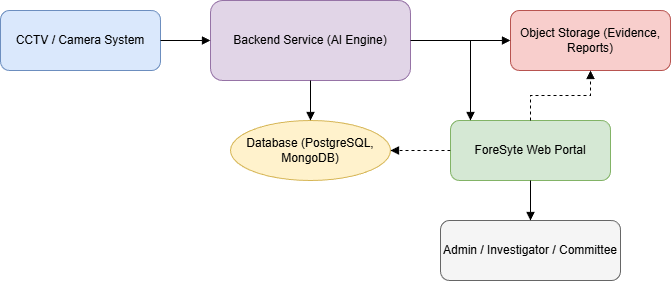
\includegraphics[width=0.85\textwidth]{sections/box-line.drawio.png}
    \caption{Box and Line Diagram for ForeSyte AI Exam Surveillance System}
    \label{fig:box-line}
\end{figure}
\FloatBarrier

\subsection{High-Level Architectural Style}
After the initial overview, the finalized architecture style/pattern diagram is presented. The system uses a two-tier client-server architecture with layered components, providing clear separation between the presentation layer (React frontend), application layer (FastAPI backend with embedded business logic), and data management layer (PostgreSQL and MongoDB). Figure~\ref{fig:architecture} illustrates the high-level architecture of the system, showing the main subsystems and their interactions.

\begin{figure}[H]
    \centering
    \caption{High-Level Architectural Design of the ForeSyte AI Exam Surveillance System}
    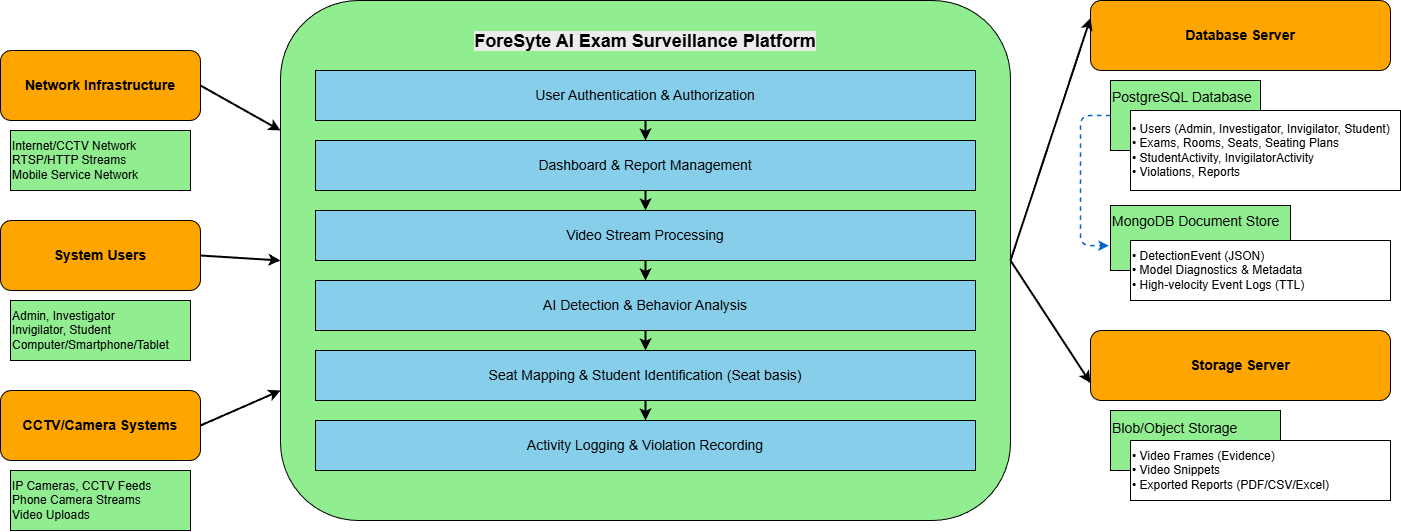
\includegraphics[width=\textwidth]{sections/foresyte-architecture-style.drawio.png}
    \label{fig:architecture}
\end{figure}
\FloatBarrier

\subsection{Mapping of Modules/Components}
Each module/component is mapped to its respective part of the architecture, ensuring modularity and scalability. The architecture supports integration with external systems (CCTV, storage, databases) and provides a robust foundation for AI-powered exam monitoring.

\section{Data Design}

The data design for \textbf{ForeSyte} focuses on how the system's information domain is represented and transformed into data structures across relational, document, and object stores. In this section, we outline the major system entities, how they are stored, processed, and managed to ensure robust operation and secure handling of user information and evidence.

\subsection{Data Structures and Organization}
ForeSyte deals with multiple data classes: user identities, seating plans, live/recorded video evidence, AI detections, activities, violations, and reports. The core data is organized so that:
\begin{itemize}
  \item \textbf{Relational (PostgreSQL)} holds normalized, queryable facts: Users, Exams, Rooms, Seats, StudentActivity, InvigilatorActivity, Violations, Reports, and seat assignments; enforced with foreign keys.
  \item \textbf{Document (MongoDB)} holds high-velocity \textit{DetectionEvent} JSON and model diagnostics with TTL, enabling fast ingest and optional replay/debug.
  \item \textbf{Blob/Object Storage} (evidence bucket) stores immutable artifacts: frame crops, video snippets, and exported PDF reports.
\end{itemize}

\paragraph{Data lifecycle.} Streams or uploads produce detection events; an aggregation service converts them into activities and violations with evidence links; dashboards and investigators read relational views and open the referenced evidence in object storage.

\subsection{Major Data Entities}
Key logical entities:
\begin{itemize}
  \item \textbf{User Information}: Admin, Invigilator, Investigator, and Student profiles with credentials and roles.
  \item \textbf{Exam/Room/Seat}: Exam sessions; rooms with cameras; seats mapped to students and exams.
  \item \textbf{DetectionEvent} (document): Raw detector output with timestamps, camera/room source, and model metadata.
  \item \textbf{StudentActivity/InvigilatorActivity}: Curated activities derived from detections; include severity, confidence, and optional evidence URL.
  \item \textbf{Violation}: Confirmed cheating events; include type, timestamp, severity, status, and optional evidence URL.
  \item \textbf{Report}: Generated summaries (PDF) of violations and activities for investigators.
\end{itemize}
\vspace{-0.5em} % ↓ Tightens space before the next heading

\subsection{Data Flow Diagrams (DFDs)}
\vspace{-0.25em} % ↓ Minimizes gap under heading

This subsection presents the logical data flow within the ForeSyte system at two abstraction levels.
Level 0 provides an overview of the main system interactions, while Level 1 elaborates on internal data processing — especially how seat mapping, activity detection, and behavior monitoring are interconnected.

\paragraph{Level 0 – Context Diagram}
Figure~\ref{fig:dfd-level0} illustrates the high-level data flow between external entities (such as Students, Invigilators, and Administrators) and the ForeSyte System. It highlights how examination footage, attendance data, and violation reports circulate through the system.

\begin{figure}[htbp]
    \centering
    \caption{DFD Level 0 – ForeSyte System Context Diagram}
    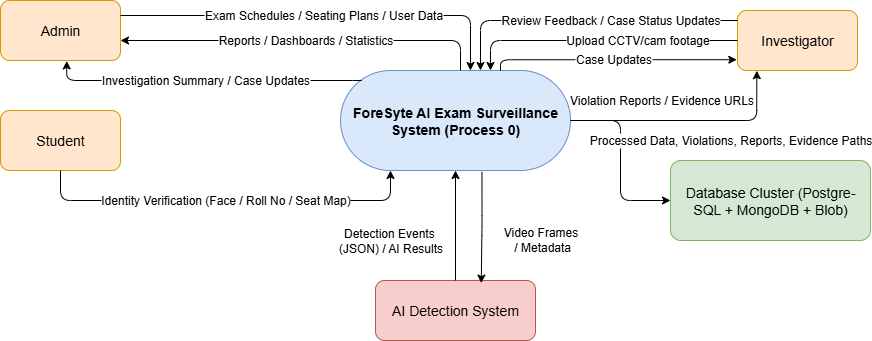
\includegraphics[width=\textwidth]{sections/DFD_Level0.drawio.png}
    \label{fig:dfd-level0}
\end{figure}


\paragraph{Level 1 – System Decomposition}
Figure~\ref{fig:dfd-level1} expands the ForeSyte process into its major internal modules: Seat Mapping, Cheating Detection Engine, Invigilator Monitoring, and Report Generation. Data from entry-point cameras are first processed to map activities to specific seats; this mapping is then propagated through subsequent modules for activity analysis and reporting.

\begin{figure}[htbp]
    \centering
    \caption{DFD Level 1 – Detailed ForeSyte System Data Flow}
    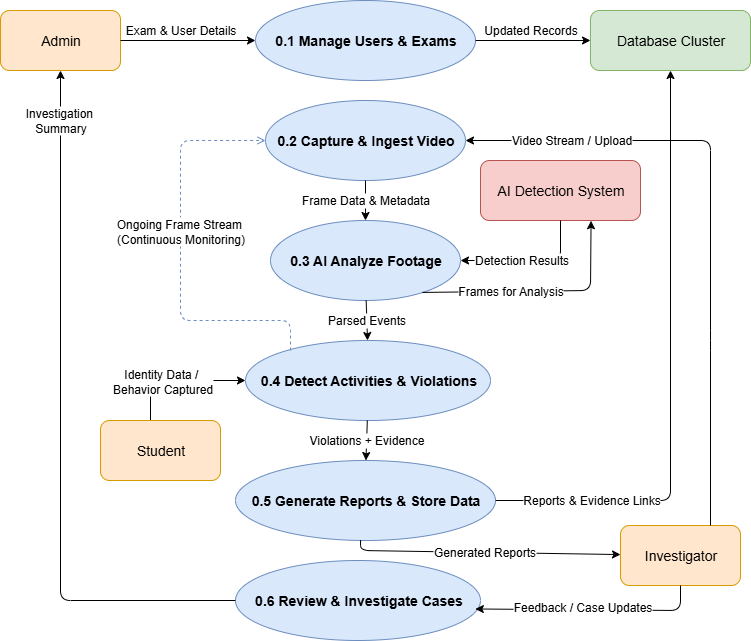
\includegraphics[width=\textwidth]{sections/DFD_Level1.drawio.png}
    \label{fig:dfd-level1}
\end{figure}
\clearpage


\subsection{Data Flow and Processing}
The system processes exam footage via two paths that converge into a unified pipeline:
\begin{enumerate}
  \item \textbf{Real-time (Live) Monitoring}: Camera streams feed the AI service, which emits per-frame \textit{DetectionEvents} (JSON).
  \item \textbf{Uploaded Footage}: After the exam, recorded video is ingested; the AI service produces the same \textit{DetectionEvents} offline.
  \item \textbf{Aggregation/Rules}: Business rules transform events into \textit{StudentActivity/InvigilatorActivity}; suspicious patterns yield \textit{Violation} rows with evidence links.
  \item \textbf{Persistence}: Normalized facts land in PostgreSQL; evidence media is stored in Blob/Object storage; optionally, transient raw events remain in MongoDB (TTL).
  \item \textbf{Consumption}: Admin dashboards query relational views; investigators open pre-signed evidence URLs and download reports.
\end{enumerate}
\let\cleardoublepage\clearpage
\section{Domain Model}
Figure \textcolor{blue}{\ref{fig:domain}} represents the domain model for ForeSyte. It outlines the key entities, their
attributes, and the relationships that define data interactions within the ForeSyte system.

\begin{figure}[htbp]
    \centering
    \caption{ForeSyte Domain Model Diagram}
    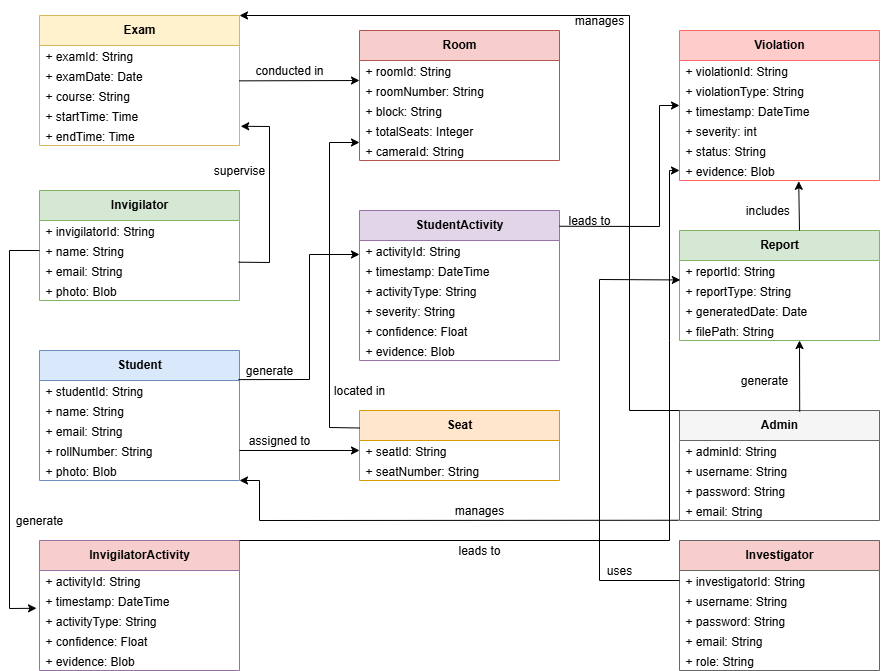
\includegraphics[width=\textwidth]{sections/domain-model.png}
    \label{fig:domain}
\end{figure}

\section{Design Models [UPTO THE CURRENT ITERATION ONLY]}

The ForeSyte system employs an object-oriented development approach, utilizing several key design models to represent the system's structure, behavior, and interactions. These models provide comprehensive documentation of the system's architecture and facilitate understanding of complex relationships between system components.

\subsection{Class Diagram}

The system's class diagram represents the core entities and their relationships within the ForeSyte domain model. 
\begin{figure}[htbp]
    \centering
    \caption{ForeSyte Class Diagram}
    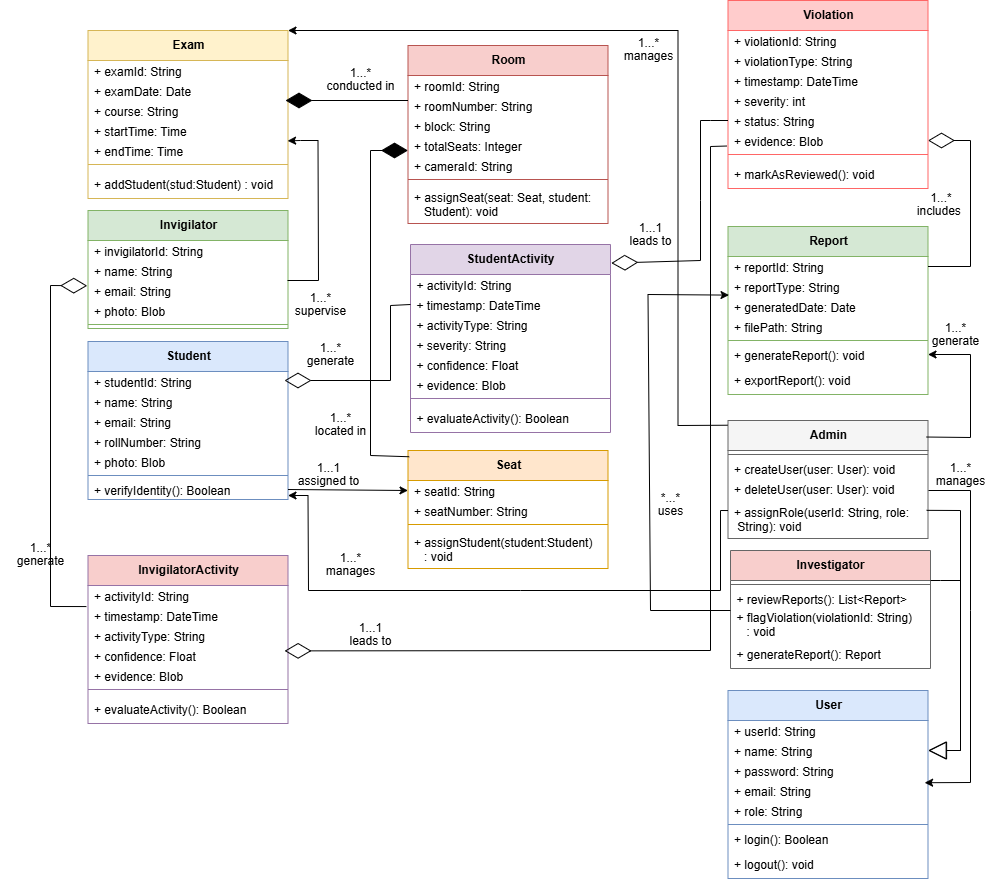
\includegraphics[width=\textwidth]{sections/class-diagram.png}
    \label{fig:class}
\end{figure}
\clearpage

\subsection{Activity Diagram}

The system's activity diagram illustrates the main processes and workflows:

\begin{figure}[H]
    \centering
    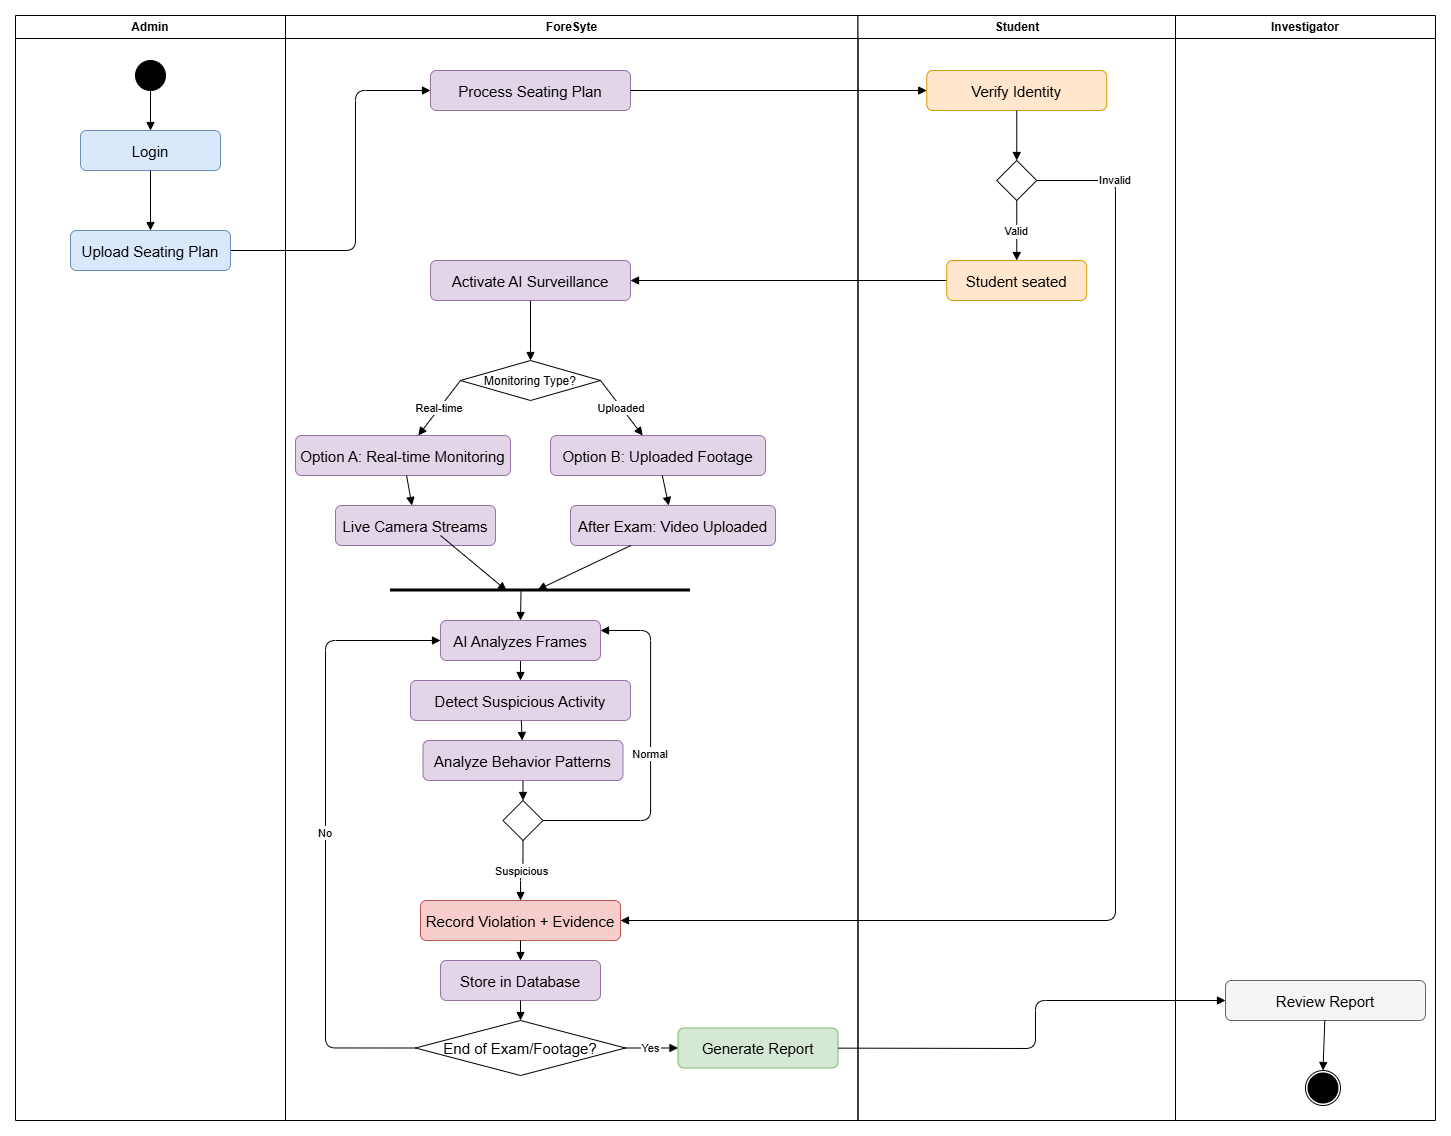
\includegraphics[width=0.95\textwidth,height=0.75\textheight,keepaspectratio]{sections/activity.png}
    \caption{ForeSyte Activity Diagram}
    \label{fig:activity}
\end{figure}
\FloatBarrier

% ------------------------
\subsection{System Sequence Diagram}

Figure~\ref{fig:ssd-foresyte} illustrates the high-level System Sequence Diagram (SSD) for ForeSyte. 
It depicts the main interactions between external actors (Students, Invigilators, Administrators, and the Discipline Committee) 
and the ForeSyte AI System across the examination workflow.  
This diagram provides an overview of how user actions trigger system processes such as attendance tagging, 
cheating detection, invigilator monitoring, and report generation.

\begin{figure}[H]
    \centering
    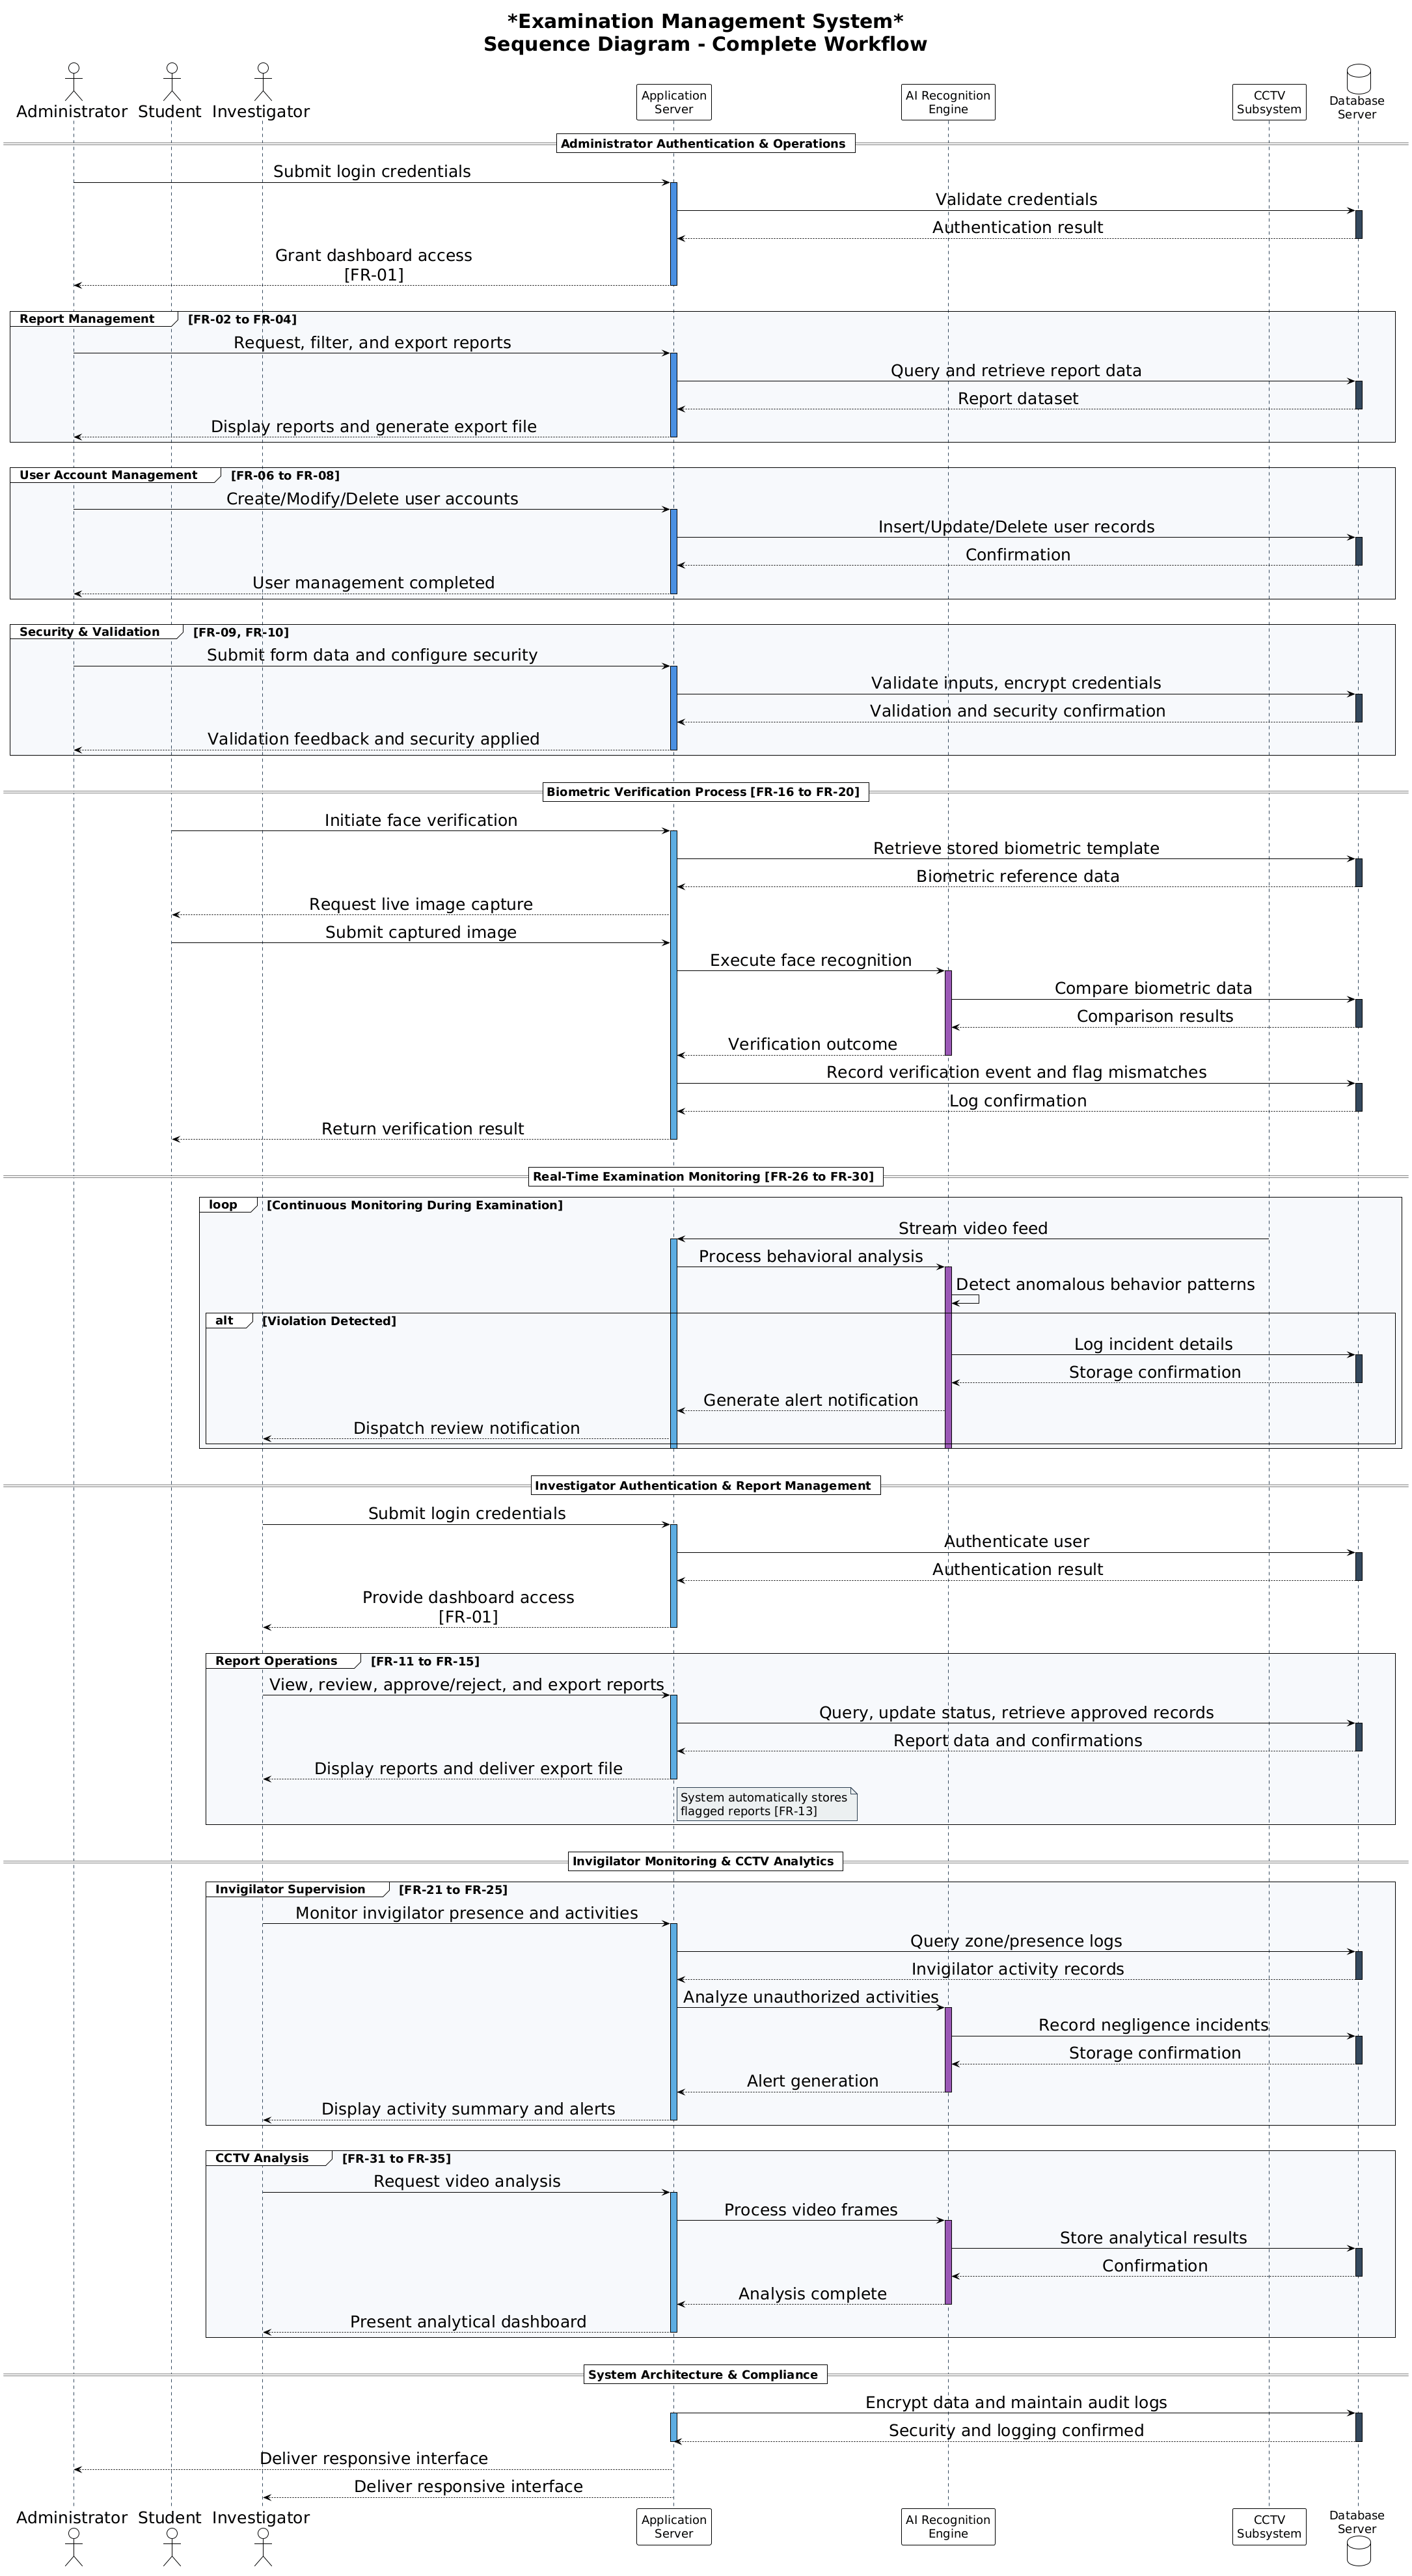
\includegraphics[width=\textwidth,height=0.85\textheight,keepaspectratio]{sections/ssd.png}
    \caption{System Sequence Diagram for ForeSyte}
    \label{fig:ssd-foresyte}
\end{figure}

% ------------------------
\subsection{Sequence Diagrams}
\vspace*{-0.5em}
This section presents the sequence diagrams for all identified use cases (UC-01 to UC-07). 
Each diagram illustrates the dynamic interaction between actors, the ForeSyte AI System, 
and domain entities.

% ---------- UC-01 ----------
\begin{figure}[H]
    \centering
    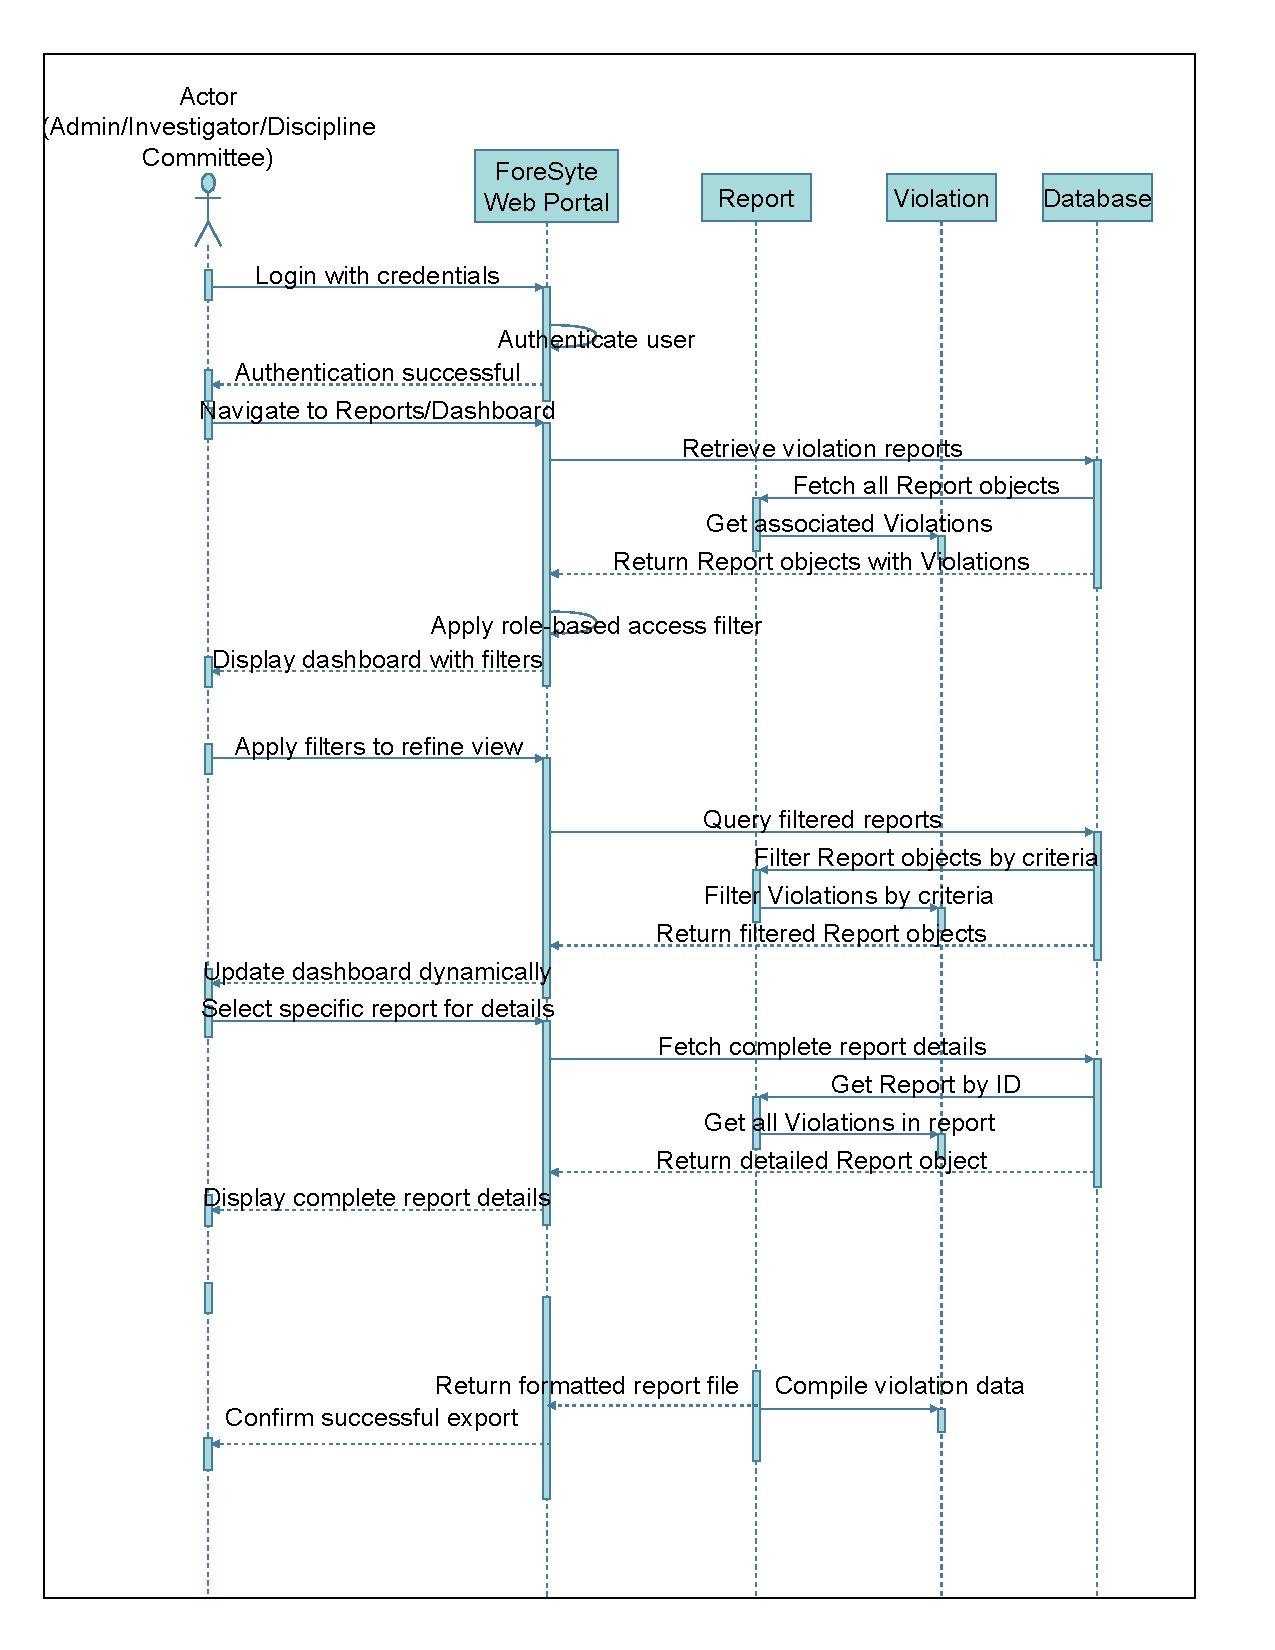
\includegraphics[width=\textwidth,height=\textheight,keepaspectratio]{sections/uc01.pdf}
    \caption{Sequence Diagram for UC-01: View and Manage Reports/Dashboard}
    \label{fig:uc01}
\end{figure}
\clearpage

% ---------- UC-02 ----------
\begin{figure}[p]
    \centering
    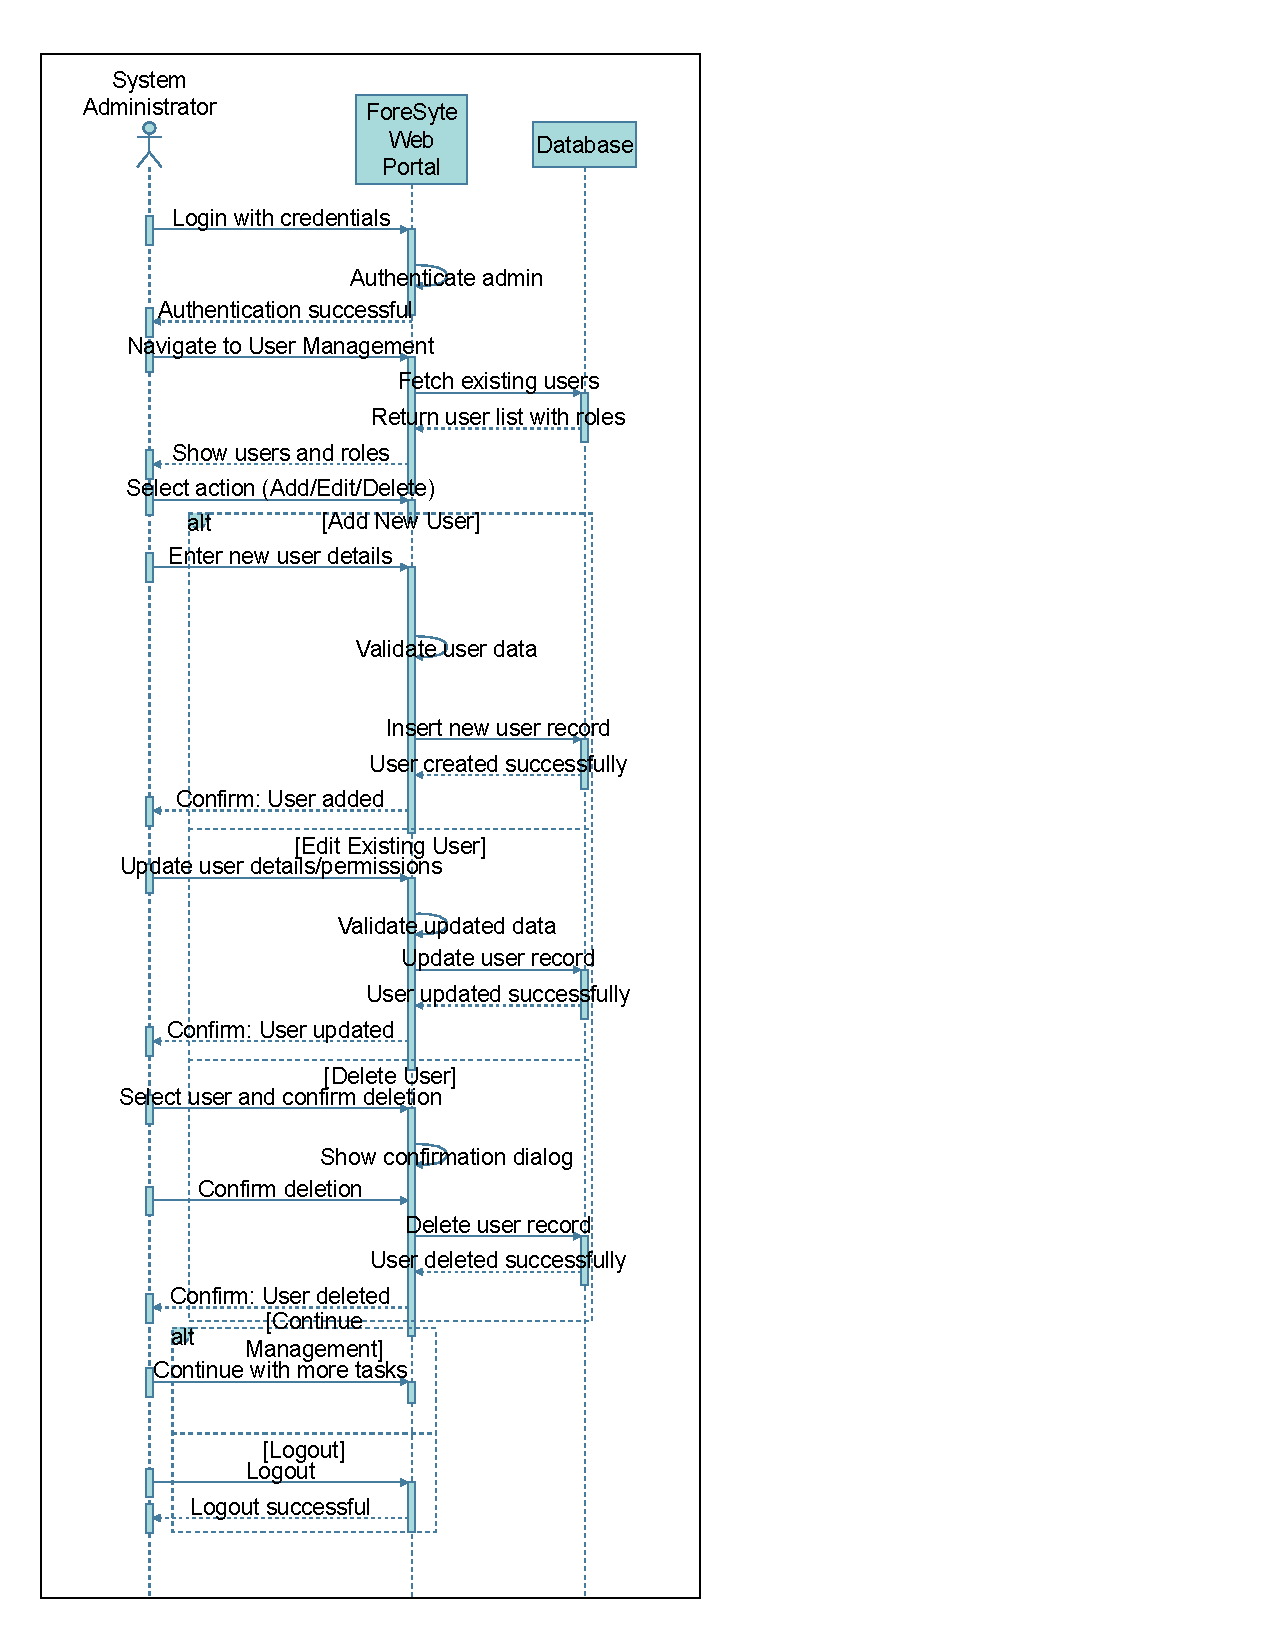
\includegraphics[width=\textwidth,height=\textheight,keepaspectratio]{sections/uc02.pdf}
    \caption{Sequence Diagram for UC-02: Manage User Profiles}
    \label{fig:uc02}
\end{figure}
\clearpage

% ---------- UC-03 ----------
\begin{figure}[p]
    \centering
    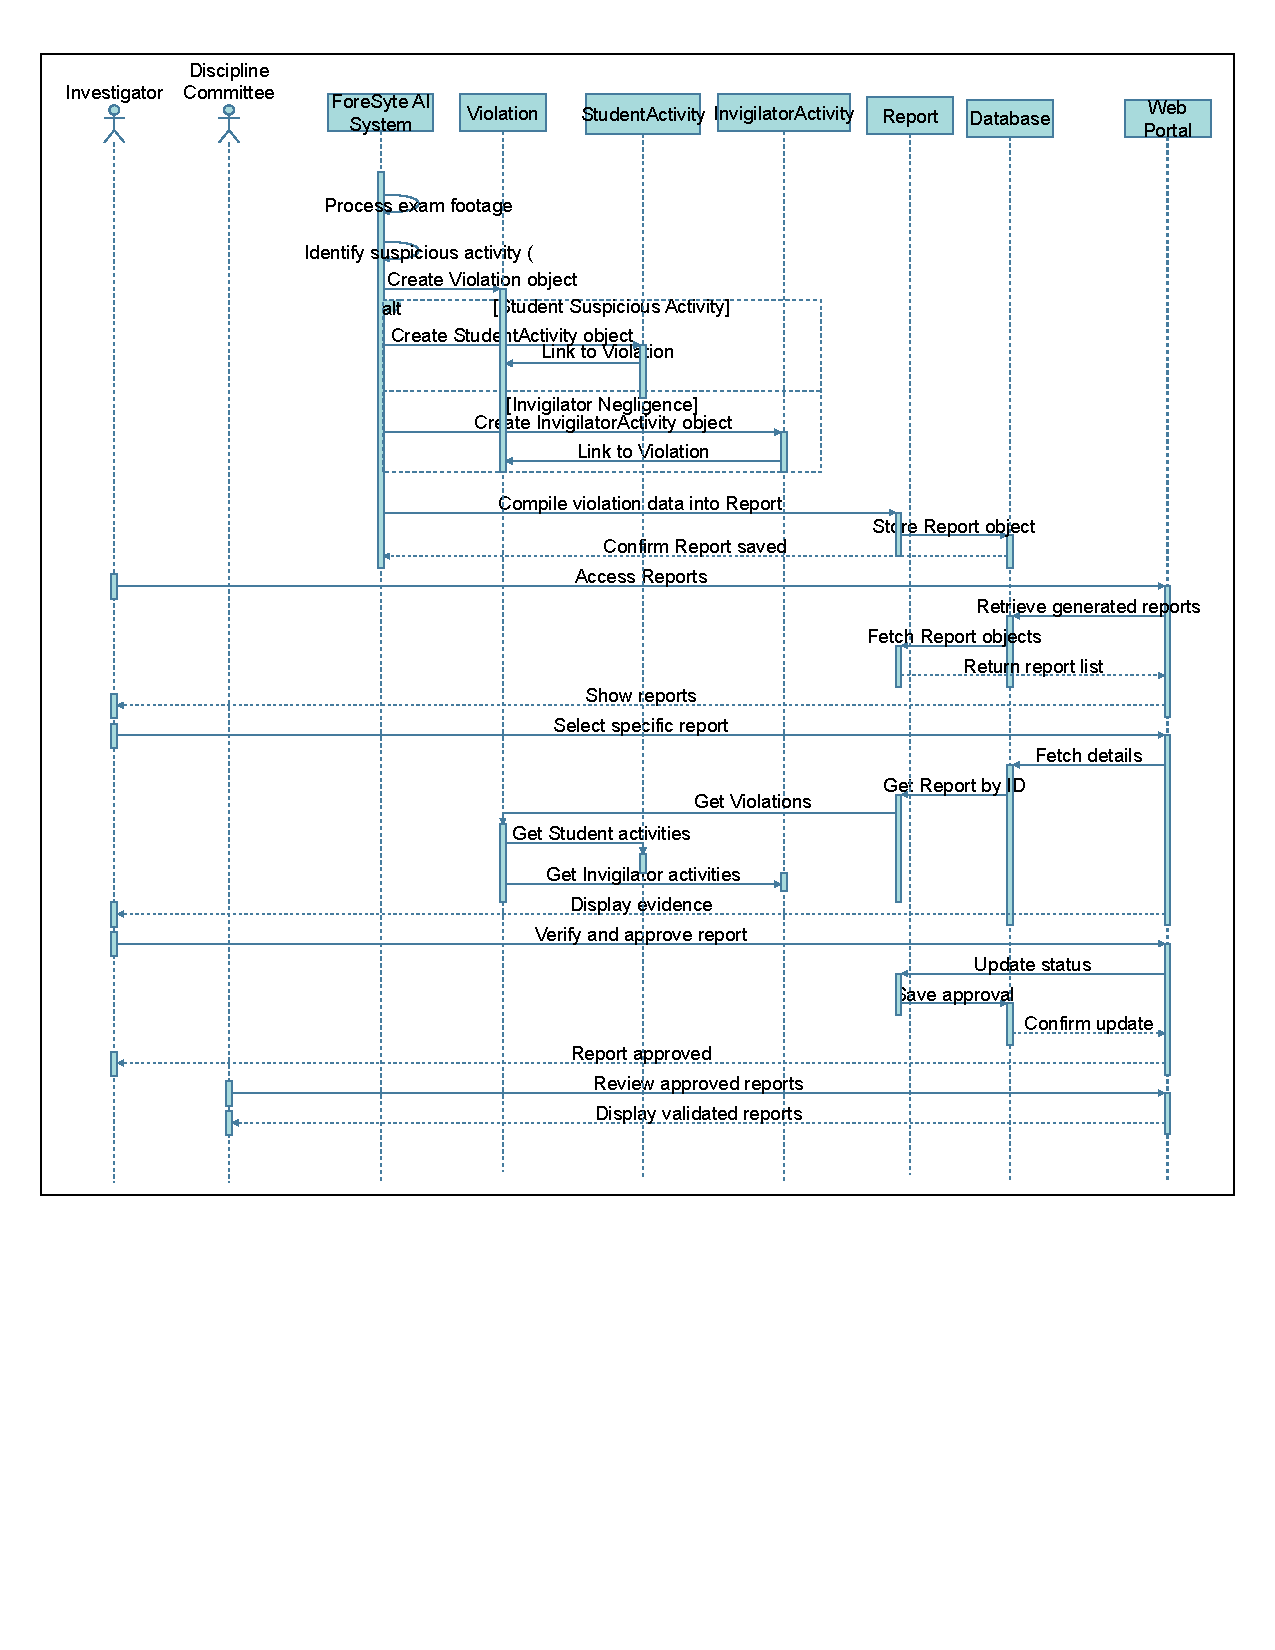
\includegraphics[width=\textwidth,height=\textheight,keepaspectratio]{sections/uc03.pdf}
    \caption{Sequence Diagram for UC-03: Generate Detection Reports}
    \label{fig:uc03}
\end{figure}
\clearpage
% ---------- UC-04 ----------
\begin{figure}[p]
    \centering
    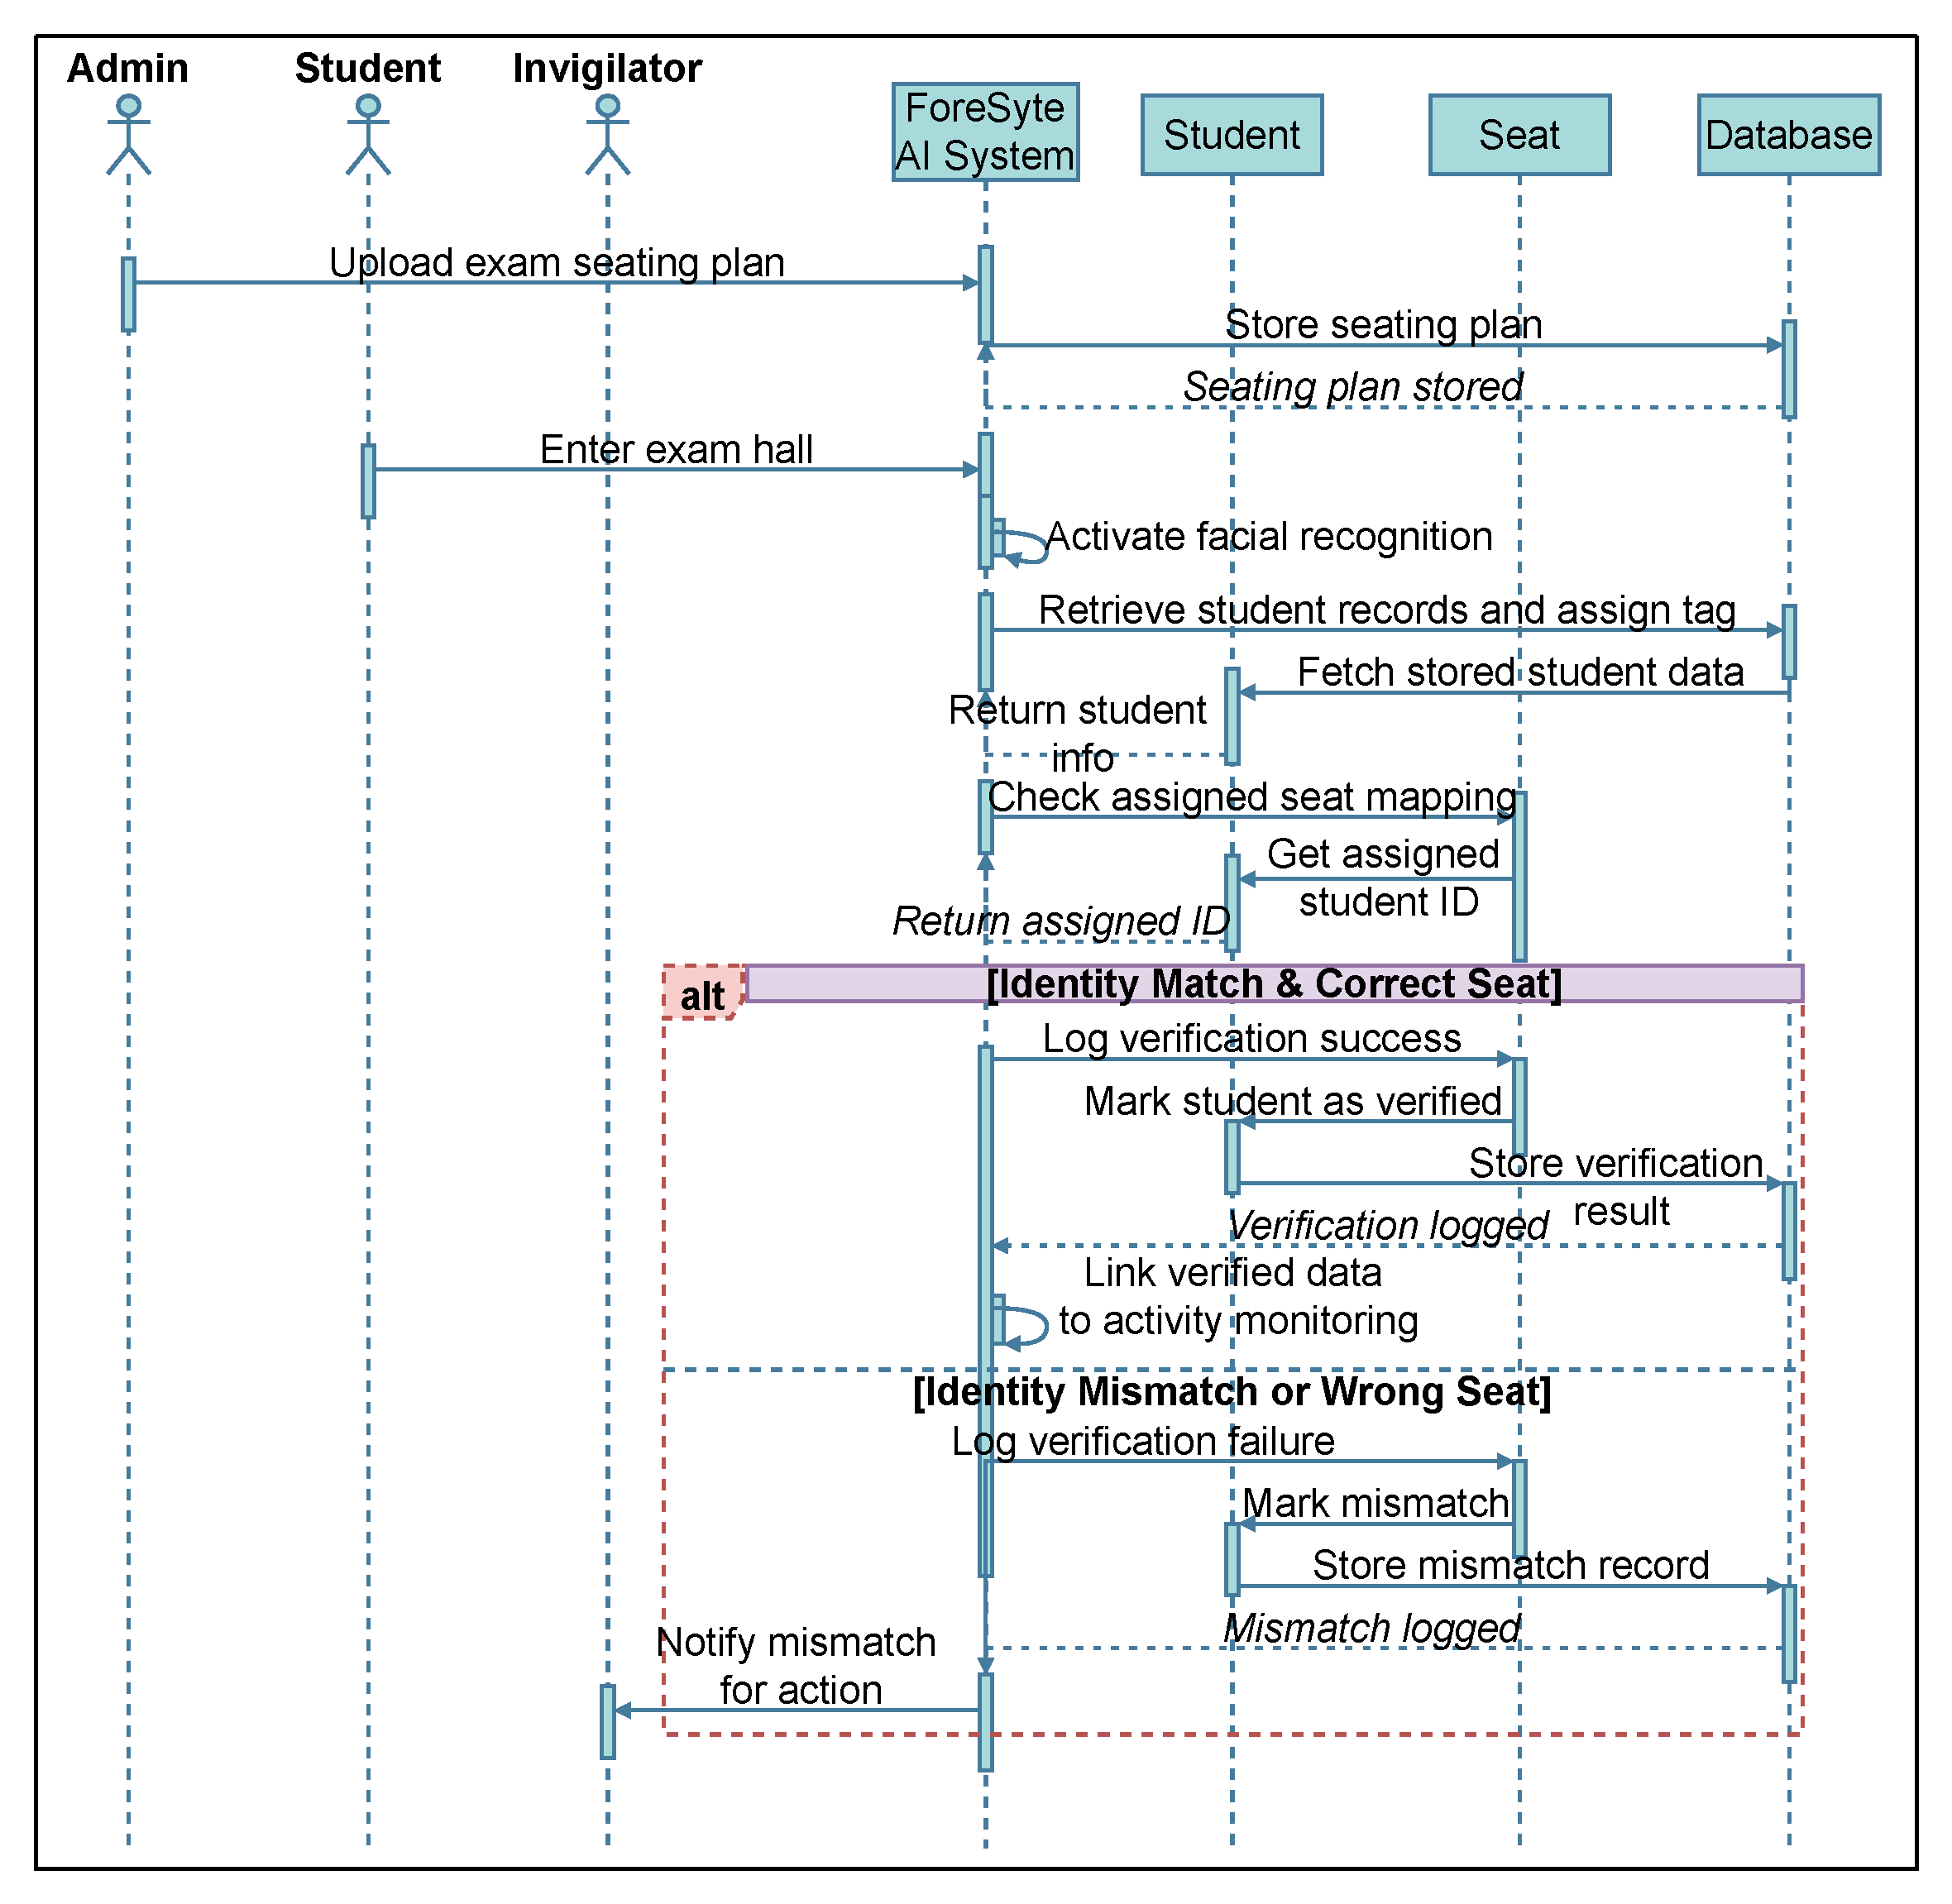
\includegraphics[width=\textwidth,height=\textheight,keepaspectratio]{sections/uc04.pdf}
    \caption{Sequence Diagram for UC-04: Verify Student Identity \& Seat Mapping}
    \label{fig:uc04}
\end{figure}
\clearpage

% ---------- UC-05 ----------
\begin{figure}[p]
    \centering
    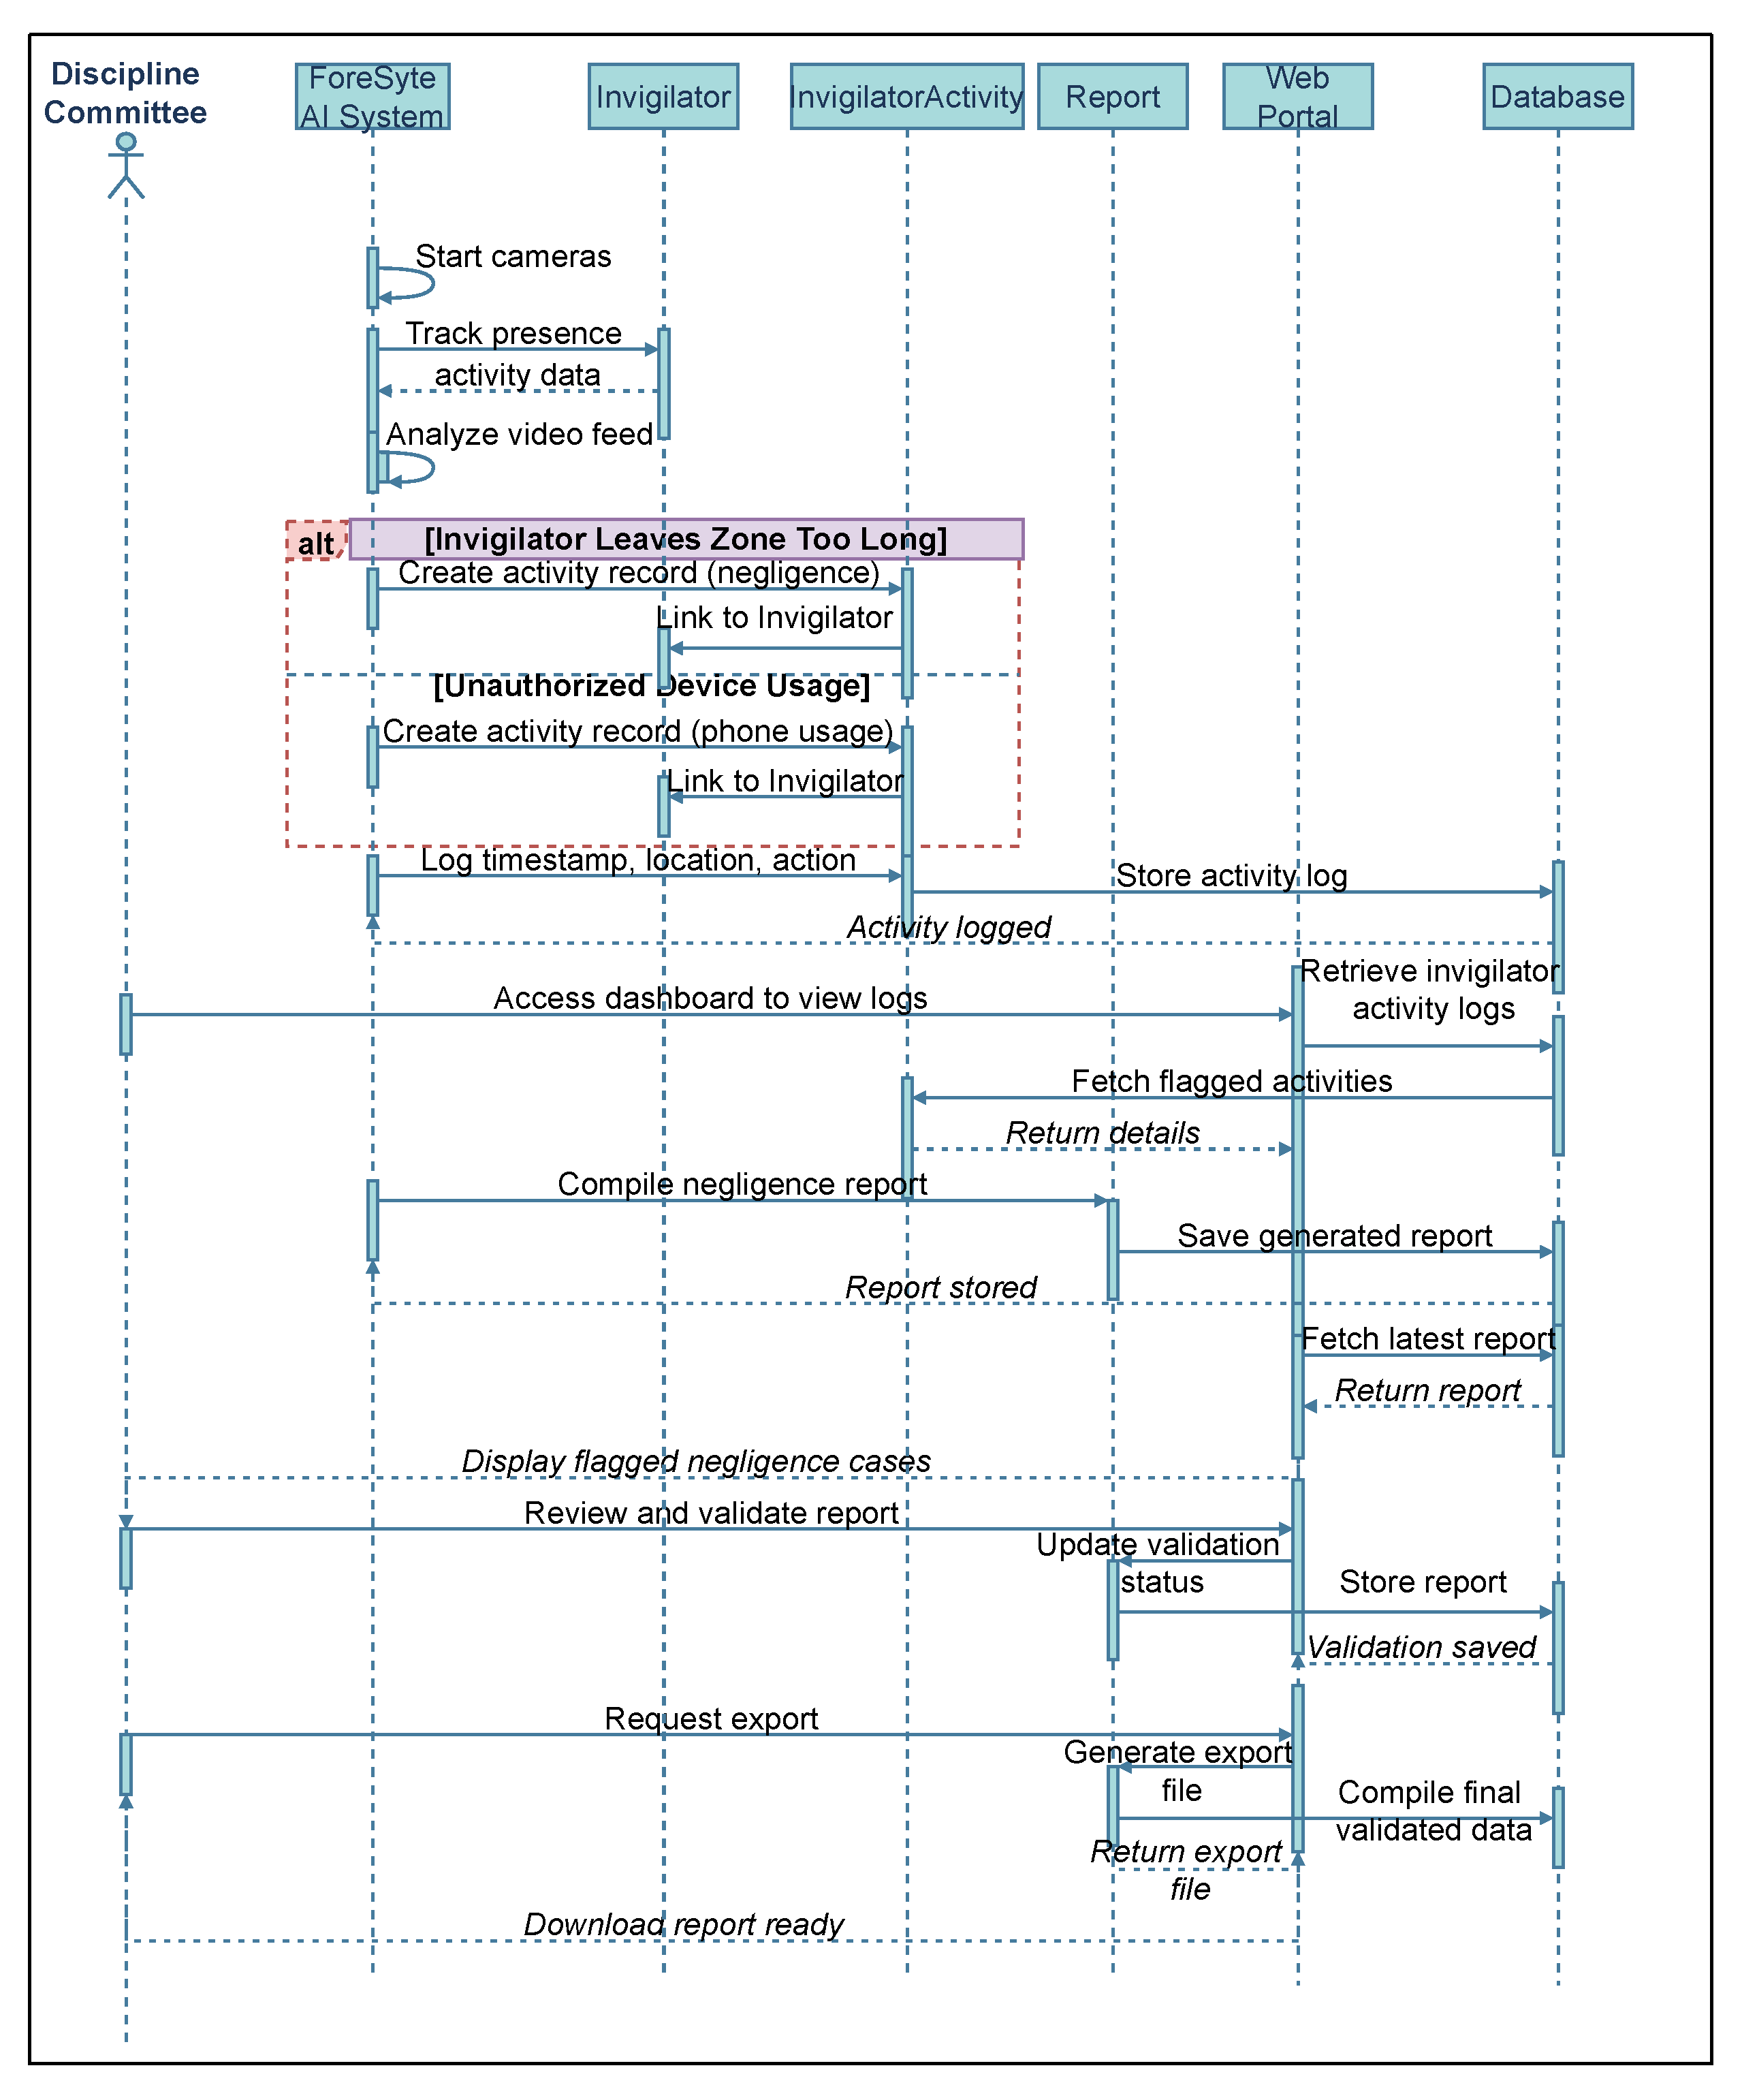
\includegraphics[width=\textwidth,height=\textheight,keepaspectratio]{sections/uc05.pdf}
    \caption{Sequence Diagram for UC-05: Monitor Invigilator Activity}
    \label{fig:uc05}
\end{figure}
\clearpage


% ---------- UC-06 ----------
\begin{figure}[p]
    \centering
 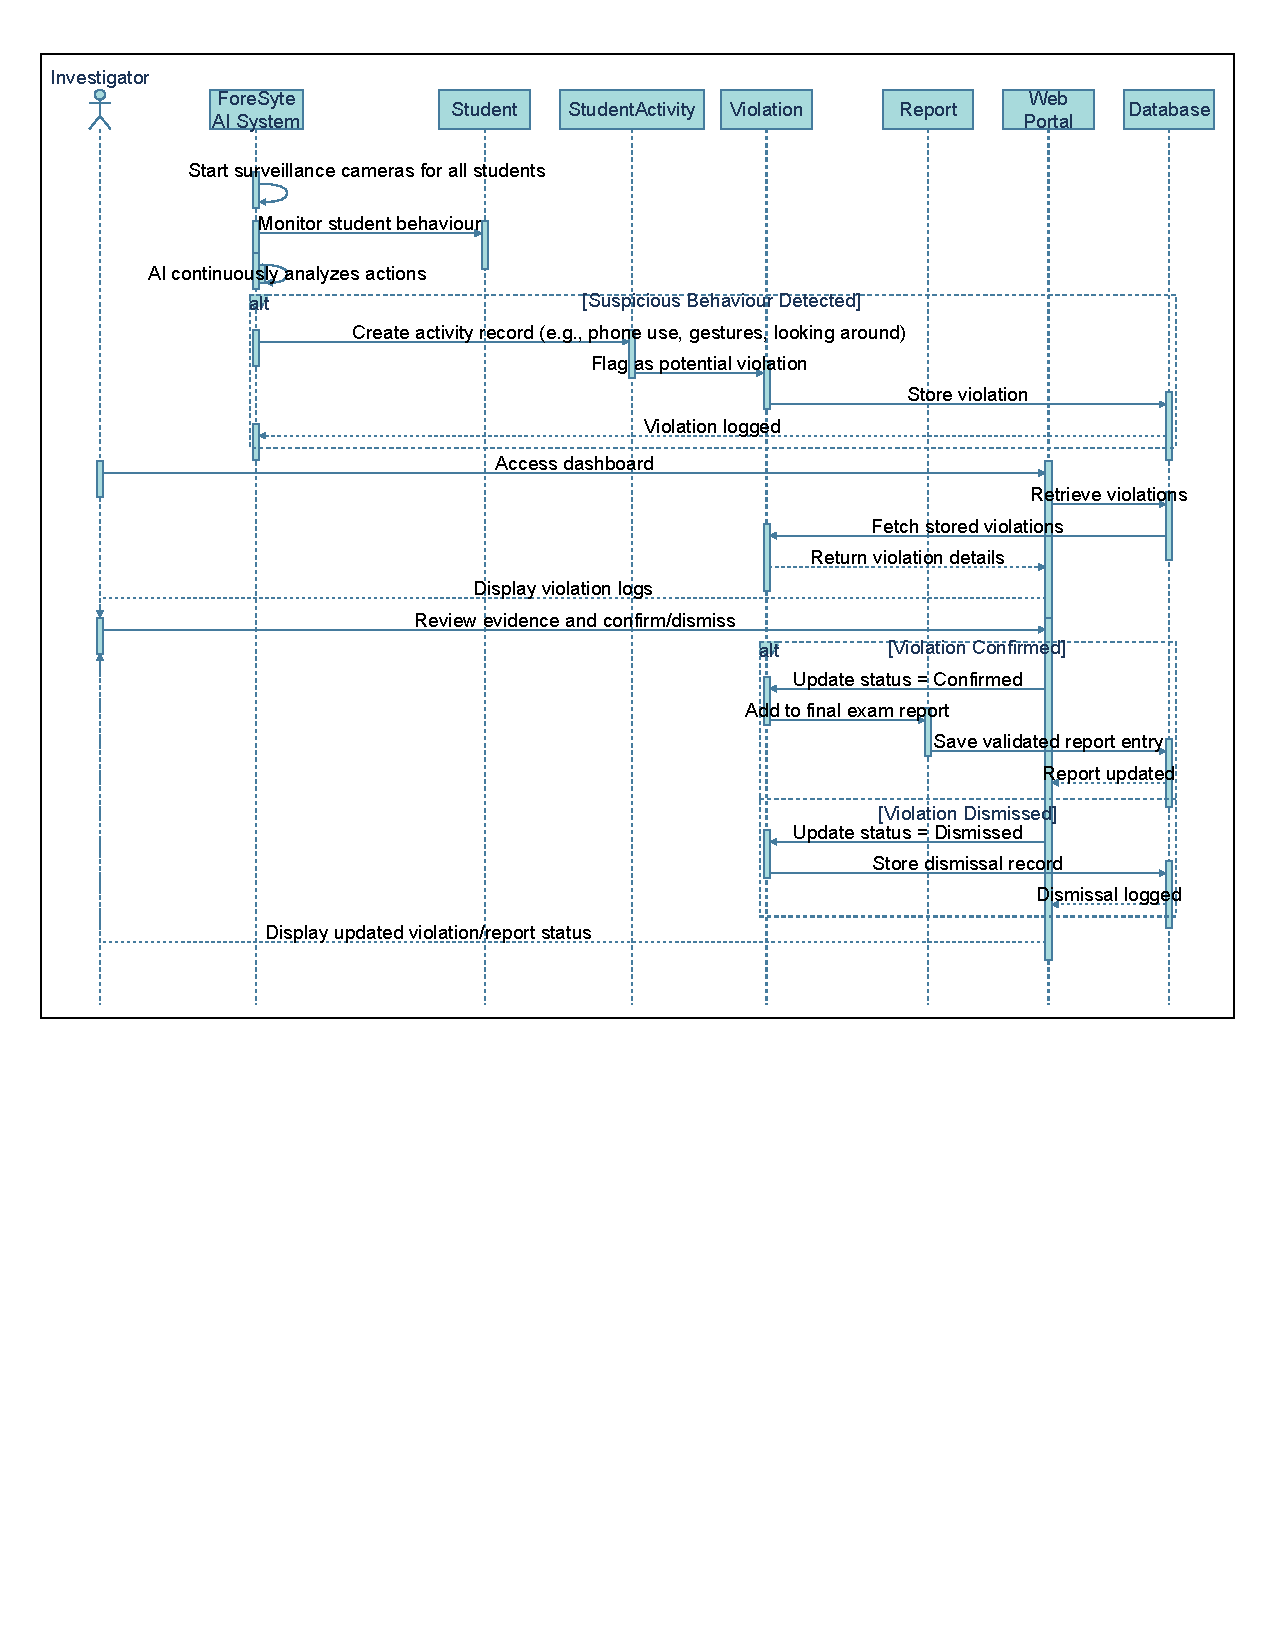
\includegraphics[width=\textwidth,height=\textheight,keepaspectratio]{sections/uc06.pdf}

    \caption{Sequence Diagram for UC-06: Monitor Student Behaviour}
    \label{fig:uc06}
\end{figure}
\clearpage

% ---------- UC-07 ----------
\begin{figure}[p]
    \centering
 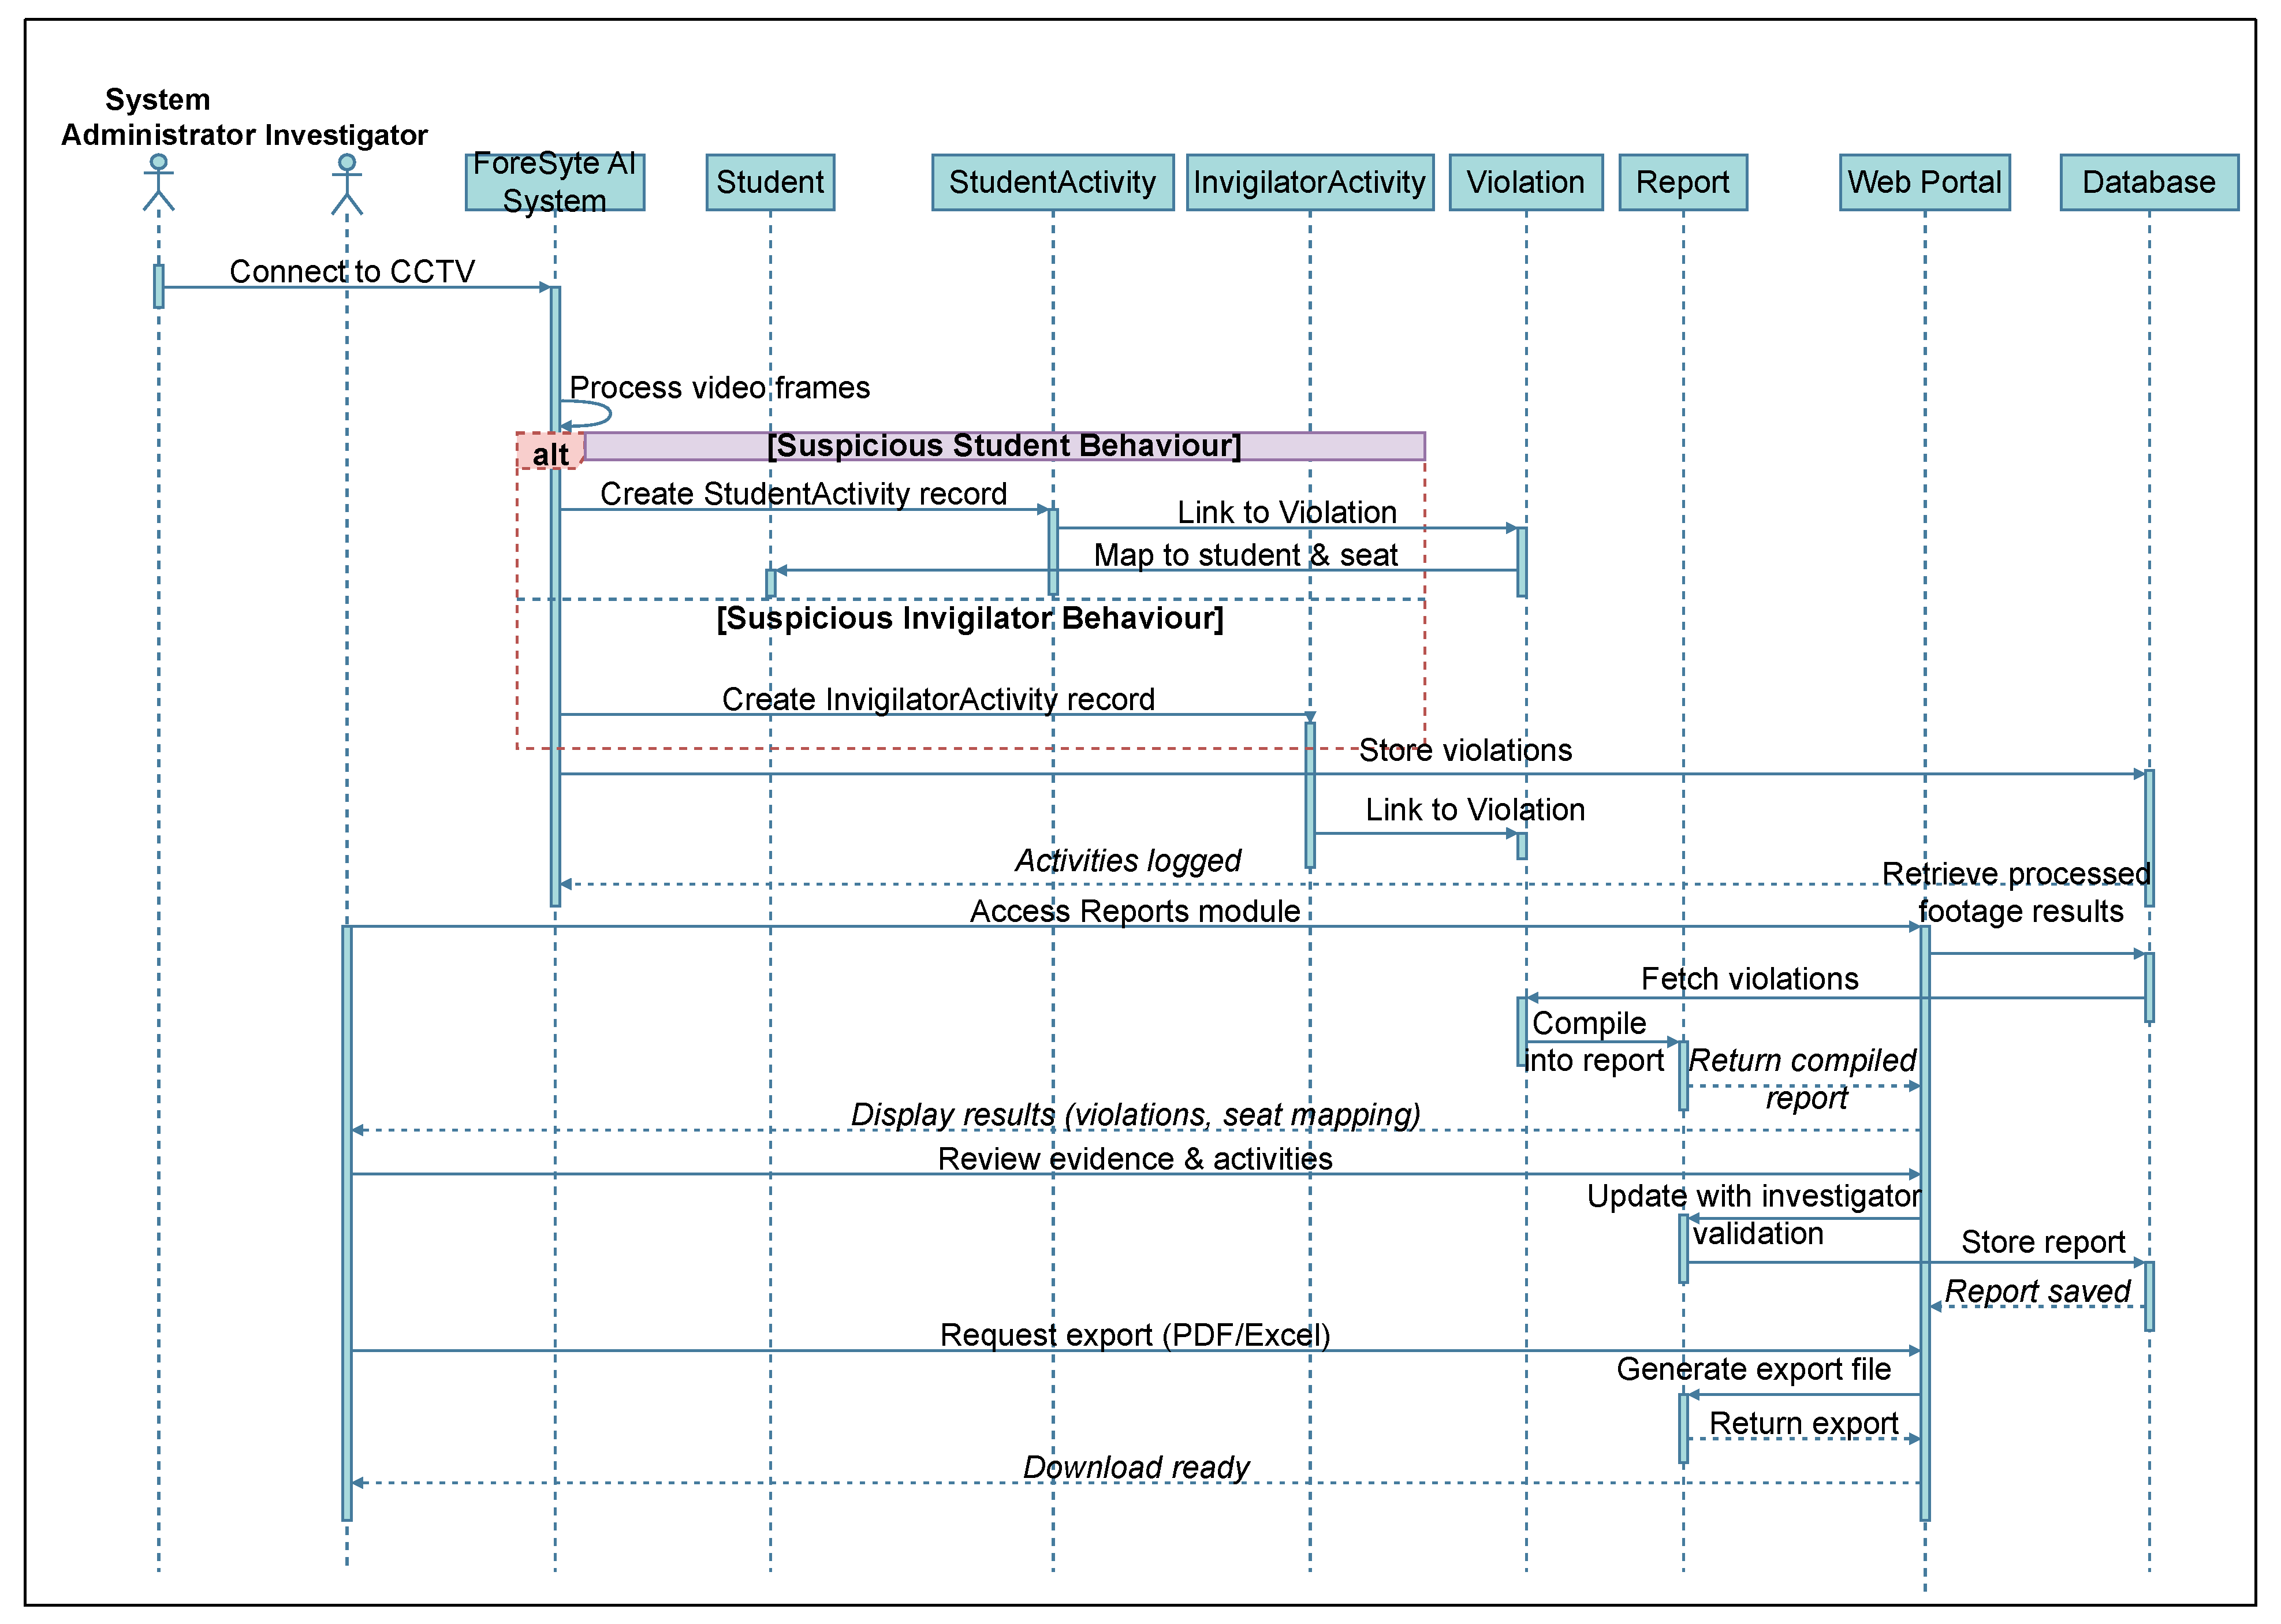
\includegraphics[width=\textwidth,height=\textheight,keepaspectratio]{sections/uc07.pdf}
    \caption{Sequence Diagram for UC-07: Process Exam Footage (Live/Recorded)}
    \label{fig:uc07}
\end{figure}
\clearpage

\subsection{State Transition Diagram}

\begin{figure}[H]
    \centering
    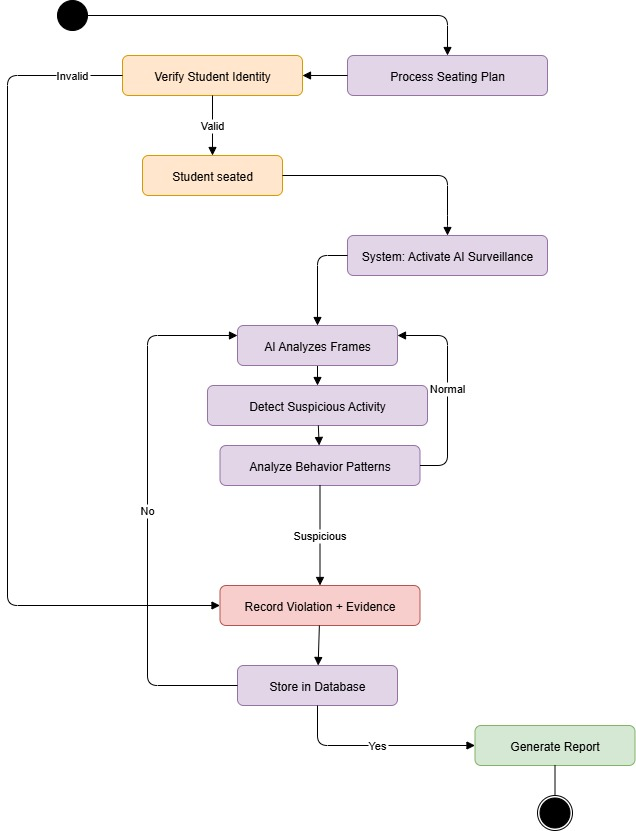
\includegraphics[width=\textwidth]{sections/std.jpg}
    \caption{State Transition Diagram}
    \label{fig:state-diagram}
\end{figure}
\FloatBarrier
This model collectively provide a comprehensive view of the ForeSyte system's architecture, ensuring clear understanding of system components, their interactions, and the overall system behavior throughout the examination monitoring process.






\chapter{Implementation and Testing}

This chapter describes the current implementation status of the \textbf{ForeSyte} AI Exam Surveillance System and the testing performed up to this iteration. The focus of this phase is on the \textbf{Admin} and \textbf{Investigator} dashboards and their supporting backend services. Computer-vision based monitoring and the Student Portal are planned components and therefore remain out of scope for this iteration.

\section{Current Progress}

\subsection{Front-End}

The front-end of ForeSyte is implemented as a modern single-page application using React, TypeScript, Vite, and Tailwind CSS. The interface is split into role-specific areas so that administrators and investigators see different dashboards and workflows.

\subsubsection*{Admin Dashboard}

The main admin dashboard presents a high-level overview of system activity. It displays:
\begin{itemize}
    \item \textbf{Active Exams} -- number of exams scheduled for the current or future dates.
    \item \textbf{Incidents Detected} -- count of student activity records (currently using placeholder data; actual cheating detection is planned for future iterations).
    \item \textbf{Students Monitored} -- number of students currently under surveillance based on seating plans and exam sessions.
    \item \textbf{Average Exam Duration} -- average exam length computed from start and end times.
\end{itemize}

These statistics are fetched via the backend \texttt{/dashboard/stats} endpoint with a period parameter (\texttt{today}, \texttt{week}, or \texttt{month}). The dashboard also includes:
\begin{itemize}
    \item An \textbf{Activity Overview} bar chart that compares the number of incidents and exams across time buckets using the \texttt{/dashboard/activity} endpoint.
    \item A \textbf{Recent Incidents} panel that lists the latest flagged student activities with severity tags using the \texttt{/dashboard/recent-incidents} endpoint.
    \item A \textbf{Quick Actions} area that links to live monitoring, reports, user management, and system settings.
    \item A \textbf{System Status} section that summarizes the health of the detection pipeline, camera network, analytics, and database.
\end{itemize}

The Admin Dashboard is therefore fully wired to the backend aggregation APIs. Loading states, error handling, and period switching are implemented in the front-end.

\subsubsection*{Investigator Portal}

The Investigator Portal is implemented as a separate area in the React application, with its own header and sidebar components to clearly separate workflows from the admin role.

\begin{itemize}
    \item The \textbf{Investigator Dashboard} displays summary cards for total violations, pending reviews, violations resolved today, and active exams. It also lists recent activities (e.g., phone usage, invigilator negligence, unauthorized movement) with severity and status badges and a period filter (\texttt{today}, \texttt{week}, \texttt{month}).
    \item The \textbf{Reports Page} shows a grid of generated reports with metadata such as report type (incident/exam), exam name, number of violations, generation date, and author. It provides filters for text search and report type, and a modal workflow for configuring a new report (type, export format, inclusion of video evidence links).
\end{itemize}

At this iteration, these investigator views use mock data to validate layout and interactions while backend report listing endpoints are being finalized. However, the UI contracts, filter behaviour, and state management are implemented and ready to be connected to live APIs.

\subsection{Back-End}

The backend is built with FastAPI and SQLAlchemy on top of PostgreSQL, with MongoDB used for flexible logging and high-volume events. Authentication uses JWT-based tokens with role-based access control (RBAC) to differentiate between Admin, Investigator, Invigilator, and Student users.

Two backend modules are particularly important for this iteration:

\begin{itemize}
    \item \textbf{Dashboard API (\texttt{/dashboard})}: aggregates data for the Admin and Investigator dashboards.
    \item \textbf{Reports API (\texttt{/reports})}: manages report generation and retrieval for incidents and exams.
\end{itemize}

\subsubsection*{Dashboard API}

The \texttt{/dashboard/stats} endpoint computes:
\begin{itemize}
    \item \textbf{Active Exams}: exams scheduled for the current or future dates.
    \item \textbf{Incidents Detected}: count of \texttt{StudentActivity} records in the selected period (note: actual cheating detection via computer vision is not yet implemented; this metric reflects activity records that would be populated by the detection pipeline in future iterations).
    \item \textbf{Students Monitored}: distinct count of students with seat assignments in active exams.
    \item \textbf{Average Exam Duration}: average duration (in minutes) based on start and end times of exams in the selected period.
    \item \textbf{Trends}: percentage changes for incidents, students, and exams when compared to the previous period.
\end{itemize}

The \texttt{/dashboard/activity} endpoint returns a sequence of time buckets, each containing the number of incidents and exams in that interval. For \texttt{today}, 4-hour slots are used; for \texttt{week} and \texttt{month}, daily buckets are used. The \texttt{/dashboard/recent-incidents} endpoint returns the most recent student activities, joined with student information to show names, types, severity levels, timestamps, and model confidence values.

All dashboard endpoints enforce RBAC policies and only allow access to users with \texttt{admin} or \texttt{investigator} roles.

\subsubsection*{Reports API}

The \texttt{/reports} router provides the API structure for managing report records. \textbf{Note:} The actual file generation (PDF, CSV, Excel) is not yet implemented in this iteration; the endpoints currently create database records and return metadata, but do not produce downloadable report files.

\begin{itemize}
    \item Standard CRUD endpoints (\texttt{POST /}, \texttt{GET /}, \texttt{GET /\{id\}}, \texttt{PUT /\{id\}}, \texttt{DELETE /\{id\}}) operate on the \texttt{Report} model and validate related \texttt{Violation} and \texttt{Investigator} records. These endpoints are functional for managing report metadata.
    \item \texttt{POST /reports/incidents} accepts a list of incident IDs, desired export format, and whether to include video links. It validates and resolves the incident IDs into \texttt{StudentActivity} records, ensures there is an associated \texttt{Violation}, creates a new \texttt{Report} entry in the database, and returns a JSON response containing the report ID, file path, format, and status. \textbf{The actual report file generation (PDF/CSV/Excel) is planned for a future iteration.}
    \item \texttt{POST /reports/exams/\{exam\_id\}} is designed to generate an exam-level report by aggregating all \texttt{StudentActivity} entries for the given exam and producing a \texttt{Report} record. \textbf{Currently, this endpoint creates the database record but does not generate the actual report file.}
\end{itemize}

These APIs establish the data model and workflow structure for report management, but the actual document generation logic will be implemented in subsequent iterations.

\subsection{Next Steps}

The completed work in this iteration establishes the core dashboard infrastructure and API structure for reports. Upcoming work will:
\begin{itemize}
    \item Connect the Investigator Portal to live dashboard and report APIs instead of mock data.
    \item Implement actual report file generation (PDF, CSV, Excel) for incident and exam reports.
    \item Integrate the video processing pipeline (camera ingestion, AI models, and real-time cheating detection) into the monitoring endpoints.
    \item Finalize and expose the Student Portal, including student-facing views of violation histories and exam schedules.
\end{itemize}

\section{Algorithm Design}

This section summarizes the main algorithms and data flows used to support the implemented features in ForeSyte.

\subsection{Admin Dashboard Aggregation}

The Admin Dashboard relies on server-side aggregation logic to compute statistics for different time windows. The high-level algorithm for computing dashboard statistics is:

\begin{enumerate}
    \item \textbf{Determine Time Window:} Given \texttt{period} $\in \{\texttt{today}, \texttt{week}, \texttt{month}\}$, compute the current window (\texttt{start\_date}) and the immediately preceding window (\texttt{prev\_start}, \texttt{prev\_end}) for trend comparison.
    \item \textbf{Count Active Exams:} Query \texttt{Exam} where \texttt{exam\_date} is greater than or equal to the current date. Perform the same query on the previous window to obtain \texttt{prev\_active\_exams}.
    \item \textbf{Count Incidents and Students:} 
    \begin{itemize}
        \item Incidents: count \texttt{StudentActivity} records with timestamps within the current window.
        \item Previous incidents: count \texttt{StudentActivity} records within the previous window.
        \item Students monitored: count distinct \texttt{Seat.student\_id} in rooms and exams that fall inside the current and previous windows.
    \end{itemize}
    \item \textbf{Compute Average Exam Duration:} For all exams in the current window with non-null start and end times, compute the duration in minutes and average the result.
    \item \textbf{Compute Trends:} For each metric (incidents, students, exams), compute percentage change between current and previous counts, handling the edge case when the previous value is zero.
    \item \textbf{Return Structured Response:} Package all calculated values into a \texttt{DashboardStats} object and return it to the client.
\end{enumerate}

On the client side, the React dashboard:
\begin{itemize}
    \item Calls \texttt{/dashboard/stats} to populate the metric cards.
    \item Calls \texttt{/dashboard/activity} to render a bar chart comparing incidents and exams per time bucket.
    \item Calls \texttt{/dashboard/recent-incidents} to display the latest suspicious activities with relative time labels.
\end{itemize}

\subsection{Report Generation Workflow (Planned Design)}

The report generation workflow is designed to be configurable and format-agnostic. \textbf{Note:} The following describes the planned design; actual file generation (PDF, CSV, Excel) is not yet implemented in this iteration.

\subsubsection*{Incident Reports (Planned)}

\begin{enumerate}
    \item The investigator selects one or more incident IDs and chooses an export format (e.g., PDF, CSV, JSON), with options such as including video evidence links.
    \item The front-end constructs an \texttt{IncidentReportRequest} and sends it to \texttt{POST /reports/incidents}.
    \item The backend validates permissions, resolves the incident IDs into \texttt{StudentActivity} records, ensures there is an associated \texttt{Violation}, and generates a unique report filename.
    \item A new \texttt{Report} record is inserted in the database, and the API returns the report ID, file path, format, and status to the client. \textbf{In the current iteration, the actual report file is not generated; only the database record is created.}
\end{enumerate}

\subsubsection*{Exam Reports (Planned)}

\begin{enumerate}
    \item The investigator selects an exam and desired output format from the Reports Page.
    \item The front-end sends an \texttt{ExamReportRequest} to \texttt{POST /reports/exams/\{exam\_id\}}.
    \item The backend verifies the exam, aggregates its related \texttt{StudentActivity} records, ensures a linked \texttt{Violation} exists, and creates a \texttt{Report} entry in the database.
    \item The API responds with the report metadata. \textbf{The actual report file generation (PDF/CSV/Excel) will be implemented in a future iteration.}
\end{enumerate}

\subsection{Investigator Violation Review Flow}

The Investigator Dashboard is designed to give investigators a structured way to triage violations:

\begin{enumerate}
    \item Load dashboard summary counters (total violations, pending reviews, resolved today, active exams).
    \item Display a list of recent activities with type, severity, and status tags.
    \item Allow investigators to toggle the period filter to focus on \texttt{today}, \texttt{week}, or \texttt{month}.
    \item Provide a \textit{Review} action for each activity which, in the next iteration, will navigate to a detailed case view and allow updating violation status and adding investigation notes.
\end{enumerate}

\section{External APIs and Libraries}

At this stage, ForeSyte does not depend heavily on third-party AI services, but it makes extensive use of framework libraries and SDKs:
\begin{itemize}
    \item \textbf{FastAPI and Starlette} for HTTP routing, dependency injection, and request handling.
    \item \textbf{SQLAlchemy} and \textbf{psycopg2} for ORM and PostgreSQL connectivity.
    \item \textbf{PyMongo} for MongoDB integration in the logging and evidence pipeline.
    \item \textbf{OpenCV} and image processing libraries, which are already installed and used in internal test scripts to handle frames for future AI detectors.
    \item \textbf{React Router}, \textbf{Tailwind CSS}, and \textbf{lucide-react} on the front-end for routing, styling, and icons.
\end{itemize}

\section{Testing Details}

Testing for this iteration concentrates on validating backend APIs, role-based access control, and the correctness of aggregated statistics, along with front-end behaviour under typical and edge-case conditions.

\subsection{Unit Testing}

\subsubsection*{Reports API Tests}

Table~\ref{tab:reports-tests} summarizes representative unit tests for the Reports API.

\begin{table}[H]
    \centering
    \caption{Unit Test Cases for Reports API}
    \label{tab:reports-tests}
    \begin{tabularx}{\textwidth}{|c|X|X|X|X|X|X|X|X|}
        \hline
        \textbf{Test ID} & \textbf{Objective} & \textbf{Preconditions} & \textbf{Steps} & \textbf{Test Data} & \textbf{Expected Result} & \textbf{Postconditions} & \textbf{Actual Result} & \textbf{Pass/Fail} \\
        \hline
        TC201 & Verify admin can create a report & Valid admin JWT; existing Violation and Investigator records & Call \texttt{POST /reports} with valid payload & \texttt{report\_type}: "incident"\\\texttt{violation\_id}: valid UUID\\\texttt{generated\_by}: valid UUID & Returns \texttt{201 Created} and a Report object with non-null \texttt{report\_id} & Database contains a new Report row & As Expected & Pass \\
        \hline
        TC202 & Enforce RBAC on report creation & Authenticated investigator JWT & Call \texttt{POST /reports} with valid payload & Same as TC201 & Returns \texttt{403 Forbidden} with ``Only admins can create reports'' & No new Report row is created & As Expected & Pass \\
        \hline
        TC203 & Create report record for incidents (file generation not yet implemented) & Investigator JWT; at least one StudentActivity present & Call \texttt{POST /reports/incidents} with valid incident IDs & \texttt{incident\_ids}: [valid UUID]\\\texttt{format}: "pdf"\\\texttt{include\_video\_links}: true & Returns JSON with non-empty \texttt{id} and \texttt{file\_path}, \texttt{status = generating} & New Report row linked to a Violation exists in database (actual file generation is not yet implemented) & As Expected & Pass \\
        \hline
        TC204 & Handle invalid incident IDs gracefully & Investigator JWT & Call \texttt{POST /reports/incidents} with invalid IDs & \texttt{incident\_ids}: ["invalid-uuid"]\\\texttt{format}: "csv" & Returns \texttt{404 Not Found} with ``No valid incidents found'' & No Report row is created & As Expected & Pass \\
        \hline
    \end{tabularx}
\end{table}

\subsubsection*{Dashboard API Tests}

Table~\ref{tab:dashboard-tests} lists key unit tests for the dashboard statistics and recent incidents endpoints.

\begin{table}[H]
    \centering
    \caption{Unit Test Cases for Dashboard APIs}
    \label{tab:dashboard-tests}
    \begin{tabularx}{\textwidth}{|c|X|X|X|X|X|X|X|X|}
        \hline
        \textbf{Test ID} & \textbf{Objective} & \textbf{Preconditions} & \textbf{Steps} & \textbf{Test Data} & \textbf{Expected Result} & \textbf{Postconditions} & \textbf{Actual Result} & \textbf{Pass/Fail} \\
        \hline
        TC301 & Retrieve ``today'' dashboard stats & Admin JWT; at least one exam scheduled today & Call \texttt{GET /dashboard/stats?period=today} & \texttt{period}: "today" & Returns a valid \texttt{DashboardStats} object; all counts are non-negative and consistent with seeded data & Values computed from sample database state & As Expected & Pass \\
        \hline
        TC302 & Verify period filter behaviour & Seeded data across multiple days & Call \texttt{GET /dashboard/stats} with different periods & \texttt{period}: "today", "week", "month" & Returns different counts reflecting the date range; no errors occur & Internal trend computation behaves correctly & As Expected & Pass \\
        \hline
        TC303 & Enforce RBAC on stats & Student JWT & Call \texttt{GET /dashboard/stats?period=today} & \texttt{period}: "today" & Returns \texttt{403 Forbidden} and ``Access denied'' & No sensitive stats are exposed & As Expected & Pass \\
        \hline
        TC304 & Return recent incidents list & StudentActivity rows present in DB & Call \texttt{GET /dashboard/recent-incidents?limit=5} & \texttt{limit}: 5 & Returns up to 5 incidents ordered by timestamp; each item includes ID, student name, type, severity, timestamp, and confidence & Activities are ordered from most recent to oldest & As Expected & Pass \\
        \hline
    \end{tabularx}
\end{table}

\subsubsection*{Front-End Behaviour Tests}

The front-end was validated using component-level tests and manual exploratory runs:
\begin{itemize}
    \item \textbf{Admin Dashboard Rendering:} Ensured that the metric cards, activity chart, and recent incidents list render correctly when provided with sample API responses, and that loading and empty states are displayed when data is unavailable.
    \item \textbf{Investigator Dashboard Layout:} Checked that period filters toggle correctly, summary counters are displayed, and recent activity items show appropriate severity and status chips.
    \item \textbf{Reports Page Filtering:} Verified that text search and report-type filters reduce the visible set of reports appropriately and that the ``Generate New Report'' modal captures the selected configuration.
\end{itemize}

In addition, a dedicated test script was developed for testing the phone stream ingestion and processing pipeline without enabling AI-based detection. This script validates connection to phone camera streams and basic frame capture, ensuring that the underlying streaming components are stable and ready for integration with the full monitoring pipeline in subsequent iterations. \textbf{Note:} Actual cheating detection via computer vision models is not yet implemented; the test script focuses on connectivity and frame handling only.

\subsubsection*{User Management API Tests}

Table~\ref{tab:users-tests} summarizes unit tests for the User Management API, which allows administrators to create, view, update, and delete users across all roles (Admin, Investigator, Invigilator, Student).

\begin{table}[H]
    \centering
    \caption{Unit Test Cases for User Management API}
    \label{tab:users-tests}
    \begin{tabularx}{\textwidth}{|c|X|X|X|X|X|X|X|X|}
        \hline
        \textbf{Test ID} & \textbf{Objective} & \textbf{Preconditions} & \textbf{Steps} & \textbf{Test Data} & \textbf{Expected Result} & \textbf{Postconditions} & \textbf{Actual Result} & \textbf{Pass/Fail} \\
        \hline
        TC401 & Verify admin can create a new student user & Valid admin JWT; database accessible & Call \texttt{POST /users} with student data & \texttt{name}: "John Doe"\\\texttt{email}: "john@example.com"\\\texttt{user\_type}: "student"\\\texttt{roll\_number}: "22I-1234"\\\texttt{password}: "secure123!" & Returns \texttt{201 Created} with User object containing non-null \texttt{id}, \texttt{email}, and \texttt{roll\_number} & New Student record exists in database with hashed password, email, roll\_number & As Expected & Pass \\
        \hline
        TC402 & Verify admin can create an investigator user & Valid admin JWT; database accessible & Call \texttt{POST /users} with investigator data & \texttt{name}: "Jane Smith"\\\texttt{email}: "jane@example.com"\\\texttt{user\_type}: "investigator"\\\texttt{designation}: "Senior Investigator"\\\texttt{password}: "secure123!" & Returns \texttt{201 Created} with User object containing \texttt{designation} field & New Investigator record exists in database containing designation & As Expected & Pass \\
        \hline
        TC403 & Enforce RBAC on user creation & Authenticated investigator JWT & Call \texttt{POST /users} with valid user data & Same as TC401 & Returns \texttt{403 Forbidden} with ``Only admins can create users'' & No new user record is created & As Expected & Pass \\
        \hline
        TC404 & Prevent duplicate email registration & Valid admin JWT; existing user with email ``john@example.com'' & Call \texttt{POST /users} with same email & \texttt{email}: "john@example.com"\\\texttt{user\_type}: "student" & Returns \texttt{400 Bad Request} with ``Email already registered'' & No duplicate user is created & As Expected & Pass \\
        \hline
        TC405 & Verify admin can retrieve all users with pagination & Valid admin JWT; multiple users in database & Call \texttt{GET /users?page=1\&limit=10} & \texttt{page}: 1\\\texttt{limit}: 10 & Returns \texttt{200 OK} with list of up to 10 users, total count, and pagination metadata & Response contains valid user list & As Expected & Pass \\
        \hline
        TC406 & Filter users by role & Valid admin JWT; users of different roles exist & Call \texttt{GET /users?role=student} & \texttt{role}: "student" & Returns only Student users in the response & Response contains only students & As Expected & Pass \\
        \hline
        TC407 & Verify admin can update user information & Valid admin JWT; existing non-admin user & Call \texttt{PUT /users/\{user\_id\}} with updated data & \texttt{name}: "Updated Name"\\\texttt{email}: "updated@example.com" & Returns \texttt{200 OK} with updated User object & User record reflects new name and email & As Expected & Pass \\
        \hline
        TC408 & Prevent admin from editing other admin users & Valid admin JWT; another admin user exists & Call \texttt{PUT /users/\{admin\_id\}} with update data & \texttt{name}: "Attempted Update" & Returns \texttt{403 Forbidden} with ``Admins cannot edit other admin users'' & Admin user remains unchanged & As Expected & Pass \\
        \hline
        TC409 & Verify admin can delete a non-admin user & Valid admin JWT; existing student user & Call \texttt{DELETE /users/\{user\_id\}} & Valid student \texttt{user\_id} & Returns \texttt{204 No Content} & User record is removed from database & As Expected & Pass \\
        \hline
        TC410 & Prevent deletion of admin users & Valid admin JWT; admin user exists & Call \texttt{DELETE /users/\{admin\_id\}} & Valid admin \texttt{user\_id} & Returns \texttt{403 Forbidden} or \texttt{400 Bad Request} with appropriate error message & Admin user remains in database & As Expected & Pass \\
        \hline
    \end{tabularx}
\end{table}

\subsubsection*{Seating Plan Upload Tests}

Table~\ref{tab:seating-plan-tests} lists test cases for the seating plan upload functionality, which processes PDF files containing exam schedules and extracts room, student, and seat assignment information.

\begin{table}[H]
    \centering
    \caption{Unit Test Cases for Seating Plan Upload}
    \label{tab:seating-plan-tests}
    \begin{tabularx}{\textwidth}{|c|X|X|X|X|X|X|X|X|}
        \hline
        \textbf{Test ID} & \textbf{Objective} & \textbf{Preconditions} & \textbf{Steps} & \textbf{Test Data} & \textbf{Expected Result} & \textbf{Postconditions} & \textbf{Actual Result} & \textbf{Pass/Fail} \\
        \hline
        TC501 & Upload valid seating plan PDF with room filter & Valid PDF file; admin JWT; database accessible & Call \texttt{POST /upload-seating-plan} with PDF file and room parameter & \texttt{file}: seating\_plan.pdf\\\texttt{room\_no}: "C-301" & Returns \texttt{200 OK} with extracted data including room number, exam date, time slot, and list of students with seat numbers & Room, Exam, Student, and Seat records created/updated in database & As Expected & Pass \\
        \hline
        TC502 & Upload seating plan with time slot filter & Valid PDF file; admin JWT & Call \texttt{POST /upload-seating-plan} with PDF and time slot parameter & \texttt{file}: seating\_plan.pdf\\\texttt{time\_slot}: "10:20 AM to 11:20 AM" & Returns \texttt{200 OK} with data for exams matching the specified time slot & Only matching exam data is extracted and stored & As Expected & Pass \\
        \hline
        TC503 & Handle invalid PDF file format & Admin JWT & Call \texttt{POST /upload-seating-plan} with non-PDF file & \texttt{file}: document.txt (text file) & Returns \texttt{400 Bad Request} or \texttt{422 Unprocessable Entity} with appropriate error message & No data is extracted or stored & As Expected & Pass \\
        \hline
        TC504 & Handle PDF with no matching room & Valid PDF file; admin JWT; PDF contains different rooms & Call \texttt{POST /upload-seating-plan} with non-existent room & \texttt{file}: seating\_plan.pdf\\\texttt{room\_no}: "Z-999" & Returns \texttt{404 Not Found} or \texttt{400 Bad Request} indicating room not found in PDF & No database changes occur & As Expected & Pass \\
        \hline
        TC505 & Verify automatic student creation from seating plan & Valid PDF file; admin JWT; student with roll number does not exist & Upload seating plan containing new student roll numbers & \texttt{file}: seating\_plan.pdf\\\texttt{room\_no}: "C-301" & New Student records are created with roll numbers and names from PDF; email auto-generated if not present & Student records exist in database with correct roll numbers & As Expected & Pass \\
        \hline
        TC506 & Verify seat assignment to existing students & Valid PDF file; admin JWT; student already exists in database & Upload seating plan with existing student roll numbers & \texttt{file}: seating\_plan.pdf\\existing \texttt{roll\_number}: "22I-1234" & Seat records are created/updated linking existing Student to Room with correct seat number & Seat assignment reflects in database & As Expected & Pass \\
        \hline
        TC507 & Handle large PDF file upload & Valid PDF file (>10MB); admin JWT & Call \texttt{POST /upload-seating-plan} with large PDF & \texttt{file}: large\_seating\_plan.pdf (15MB) & Returns \texttt{200 OK} after processing; or \texttt{413 Payload Too Large} if size limit enforced & File is processed or rejected based on size limits & As Expected & Pass \\
        \hline
        TC508 & Verify room creation from seating plan & Valid PDF file; admin JWT; room does not exist & Upload seating plan with new room number & \texttt{file}: seating\_plan.pdf\\\texttt{room\_no}: "D-405" & New Room record is created with room number, block, total seats, and camera ID & Room record exists in database linked to Exam & As Expected & Pass \\
        \hline
    \end{tabularx}
\end{table}

\subsubsection*{Monitoring and Camera Integration Tests}

Table~\ref{tab:monitoring-tests} presents test cases for the monitoring endpoints and camera integration functionality, which enable administrators and investigators to view live camera feeds and manage monitoring sessions.

\begin{table}[H]
    \centering
    \caption{Unit Test Cases for Monitoring and Camera Integration}
    \label{tab:monitoring-tests}
    \begin{tabularx}{\textwidth}{|c|X|X|X|X|X|X|X|X|}
        \hline
        \textbf{Test ID} & \textbf{Objective} & \textbf{Preconditions} & \textbf{Steps} & \textbf{Test Data} & \textbf{Expected Result} & \textbf{Postconditions} & \textbf{Actual Result} & \textbf{Pass/Fail} \\
        \hline
        TC601 & Retrieve monitoring feeds for all cameras & Admin JWT; rooms with cameras exist in database & Call \texttt{GET /monitoring/feeds} & No parameters & Returns \texttt{200 OK} with list of camera feeds including camera ID, room name, status, stream URL, and students monitored count & Response contains valid feed data for all rooms & As Expected & Pass \\
        \hline
        TC602 & Filter monitoring feeds by exam ID & Admin JWT; multiple exams with rooms & Call \texttt{GET /monitoring/feeds?exam\_id=\{exam\_id\}} & \texttt{exam\_id}: valid UUID & Returns only camera feeds for rooms associated with the specified exam & Response contains feeds filtered by exam & As Expected & Pass \\
        \hline
        TC603 & Enforce RBAC on monitoring feeds & Student JWT & Call \texttt{GET /monitoring/feeds} & Student token & Returns \texttt{403 Forbidden} with ``Access denied'' & No monitoring data is exposed to unauthorized users & As Expected & Pass \\
        \hline
        TC604 & Verify camera status endpoint & Admin JWT; camera exists & Call \texttt{GET /monitoring/cameras/\{camera\_id\}/status} & \texttt{camera\_id}: valid camera ID & Returns \texttt{200 OK} with camera status including last heartbeat, students detected, and connection status & Response contains valid status information & As Expected & Pass \\
        \hline
        TC605 & Handle non-existent camera ID & Admin JWT & Call \texttt{GET /monitoring/cameras/invalid-id/status} & \texttt{camera\_id}: "invalid-id" & Returns \texttt{404 Not Found} with appropriate error message & No data is returned & As Expected & Pass \\
        \hline
        TC606 & Start phone camera monitoring session & Admin JWT; phone stream URL available & Call \texttt{POST /phone-monitoring/start} with stream URL & \texttt{stream\_url}: "http://192.168.1.100:8080/video"\\\texttt{exam\_id}: "exam-123"\\\texttt{duration\_seconds}: 3600 & Returns \texttt{200 OK} with \texttt{session\_id}, \texttt{status: "started"}, and confirmation message & Monitoring session is active; frames are being captured & As Expected & Pass \\
        \hline
        TC607 & Verify phone monitoring session status & Admin JWT; active monitoring session exists & Call \texttt{GET /phone-monitoring/\{session\_id\}/status} & \texttt{session\_id}: valid session ID & Returns \texttt{200 OK} with session status including frames captured, processing status, and duration & Response reflects current monitoring state & As Expected & Pass \\
        \hline
        TC608 & Stop active phone monitoring session & Admin JWT; active monitoring session exists & Call \texttt{POST /phone-monitoring/\{session\_id\}/stop} & \texttt{session\_id}: valid session ID & Returns \texttt{200 OK} with \texttt{status: "stopped"} and confirmation message & Monitoring session is terminated; no further frames captured & As Expected & Pass \\
        \hline
        TC609 & Handle invalid stream URL in phone monitoring & Admin JWT & Call \texttt{POST /phone-monitoring/start} with invalid URL & \texttt{stream\_url}: "http://invalid-url:8080/video" & Returns \texttt{400 Bad Request} or connection error indicating invalid stream URL & No monitoring session is created & As Expected & Pass \\
        \hline
        TC610 & Verify stream URL proxy endpoint & Admin JWT; valid camera stream URL exists & Call \texttt{GET /monitoring/stream-proxy?url=\{encoded\_url\}} & \texttt{url}: valid encoded stream URL & Returns proxied stream or redirects to stream source & Stream is accessible through proxy & As Expected & Pass \\
        \hline
        TC611 & Verify camera feed displays in front-end & Admin logged in; monitoring page loaded & Navigate to Monitoring page and select a camera & Camera feed with valid \texttt{stream\_url} & Camera feed displays in video/image element; status indicator shows active/inactive & UI correctly renders camera stream & As Expected & Pass \\
        \hline
        TC612 & Handle camera feed with no stream URL & Admin logged in; room exists without stream URL & Navigate to Monitoring page; select camera without \texttt{stream\_url} & Camera with \texttt{stream\_url}: null & UI displays placeholder message ``No stream URL configured'' instead of video element & UI handles missing stream gracefully & As Expected & Pass \\
        \hline
    \end{tabularx}
\end{table}

\let\cleardoublepage\clearpage


%\appendix
%\include{appendix1/appendix1}

\bibliographystyle{plain}
\bibliography{bib}
\addcontentsline{toc}{chapter}{References} 

\appendix
\appendix
\chapter{Appendices}
\section{Appendix A}

\subsection{Admin Portal Screenshots}

\subsubsection{Login Page}
\begin{figure}[H]
    \centering
    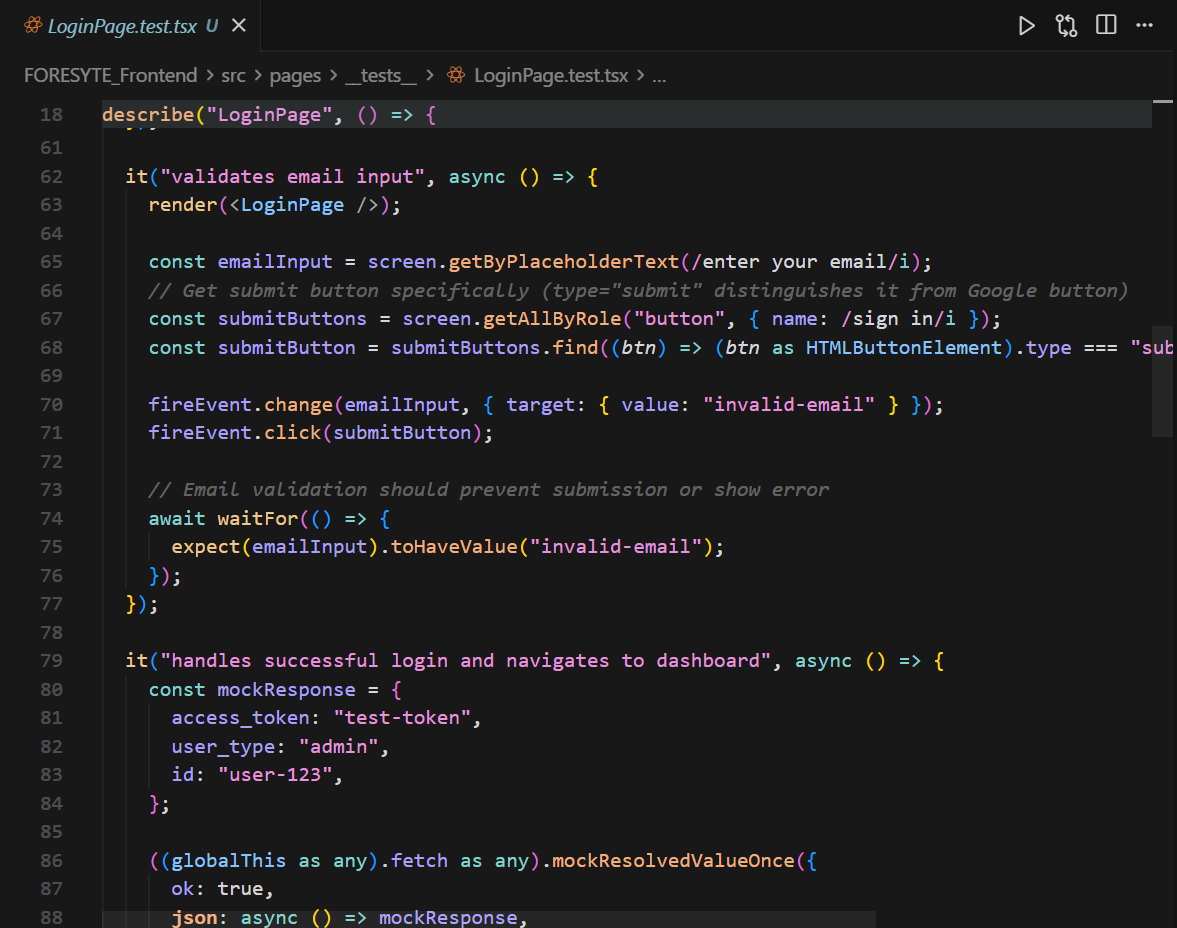
\includegraphics[width=\textwidth]{images/admin/login_page.png}
    \caption{Admin Portal Login Page}
    \label{fig:admin-login}
\end{figure}

\subsubsection{Sign Up Page}
\begin{figure}[H]
    \centering
    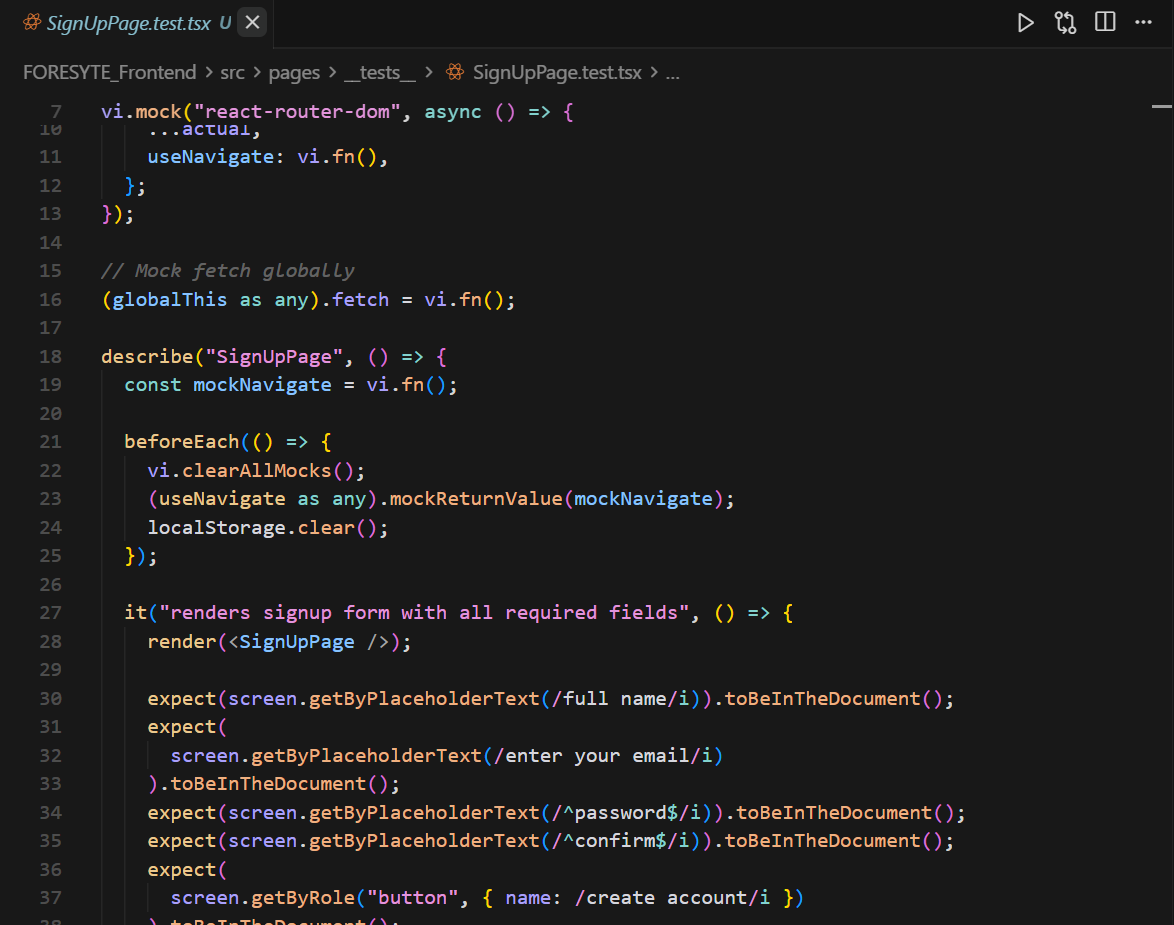
\includegraphics[width=\textwidth]{images/admin/signup_page.png}
    \caption{Admin Portal Sign Up Page}
    \label{fig:admin-signup}
\end{figure}

\subsubsection{Dashboard}
\begin{figure}[H]
    \centering
    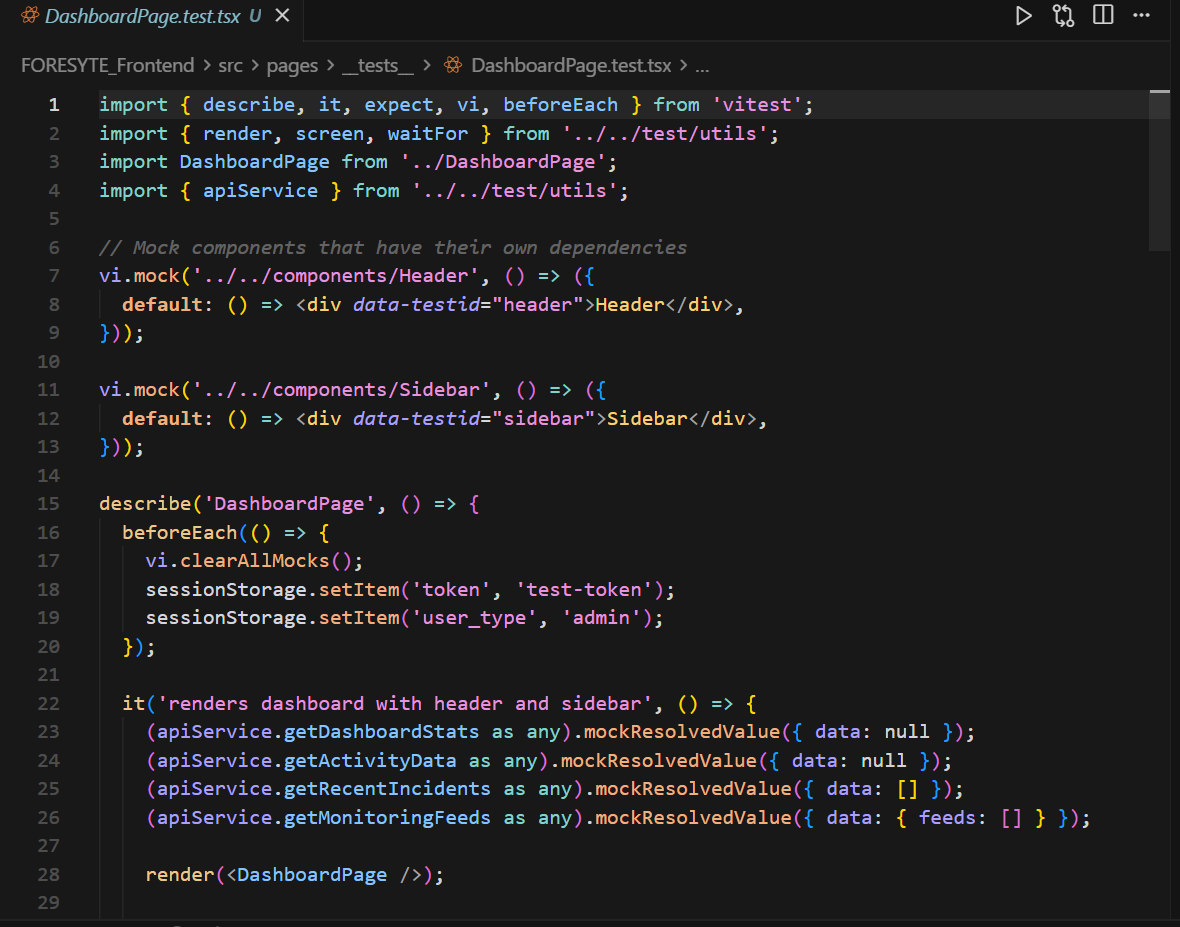
\includegraphics[width=\textwidth]{images/admin/dashboard_page.png}
    \caption{Admin Portal Dashboard}
    \label{fig:admin-dashboard}
\end{figure}

\subsubsection{Analytics Page}
\begin{figure}[H]
    \centering
    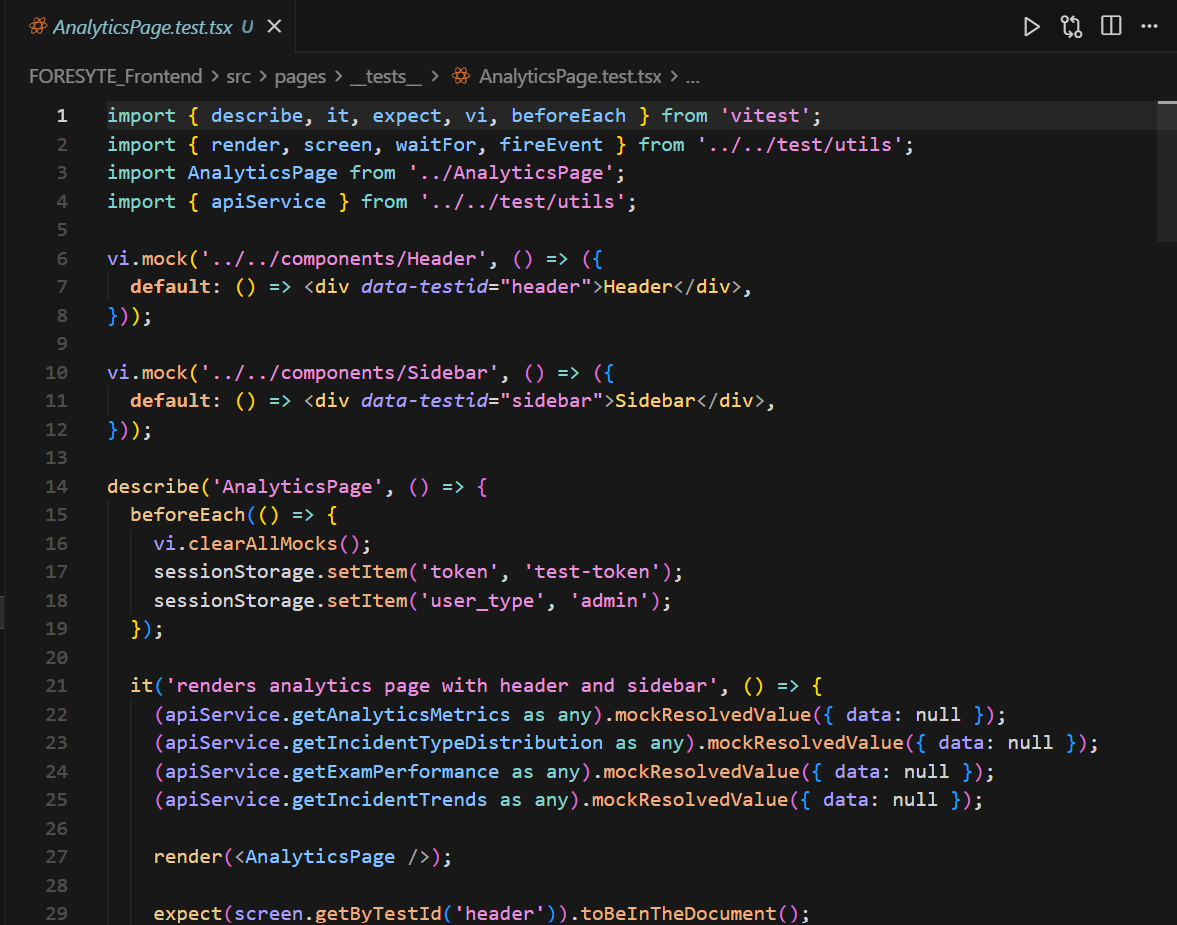
\includegraphics[width=\textwidth]{images/admin/analytics_page.png}
    \caption{Admin Portal Analytics Page}
    \label{fig:admin-analytics}
\end{figure}

\subsubsection{Exams Page}
\begin{figure}[H]
    \centering
    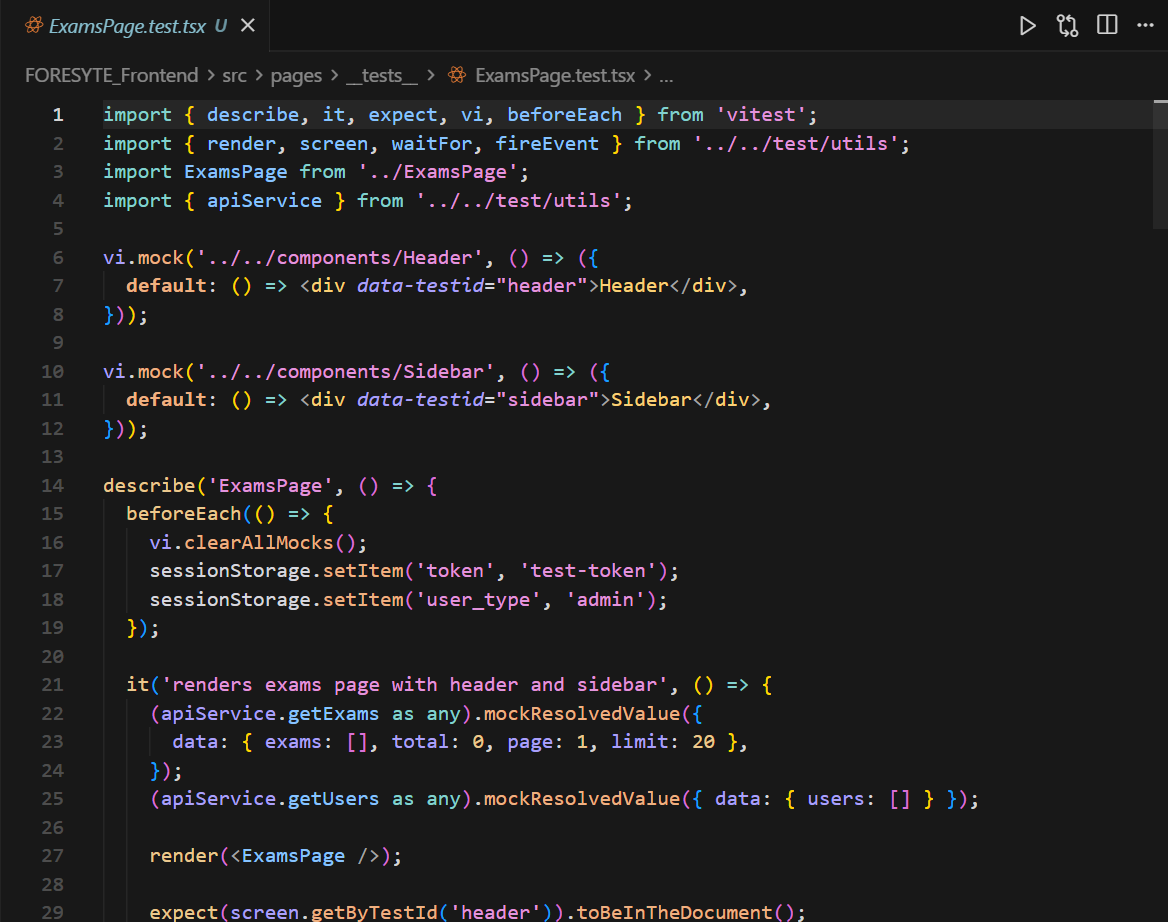
\includegraphics[width=\textwidth]{images/admin/exams_page.png}
    \caption{Admin Portal Exams Management Page}
    \label{fig:admin-exams}
\end{figure}

\subsubsection{Users Page}
\begin{figure}[H]
    \centering
    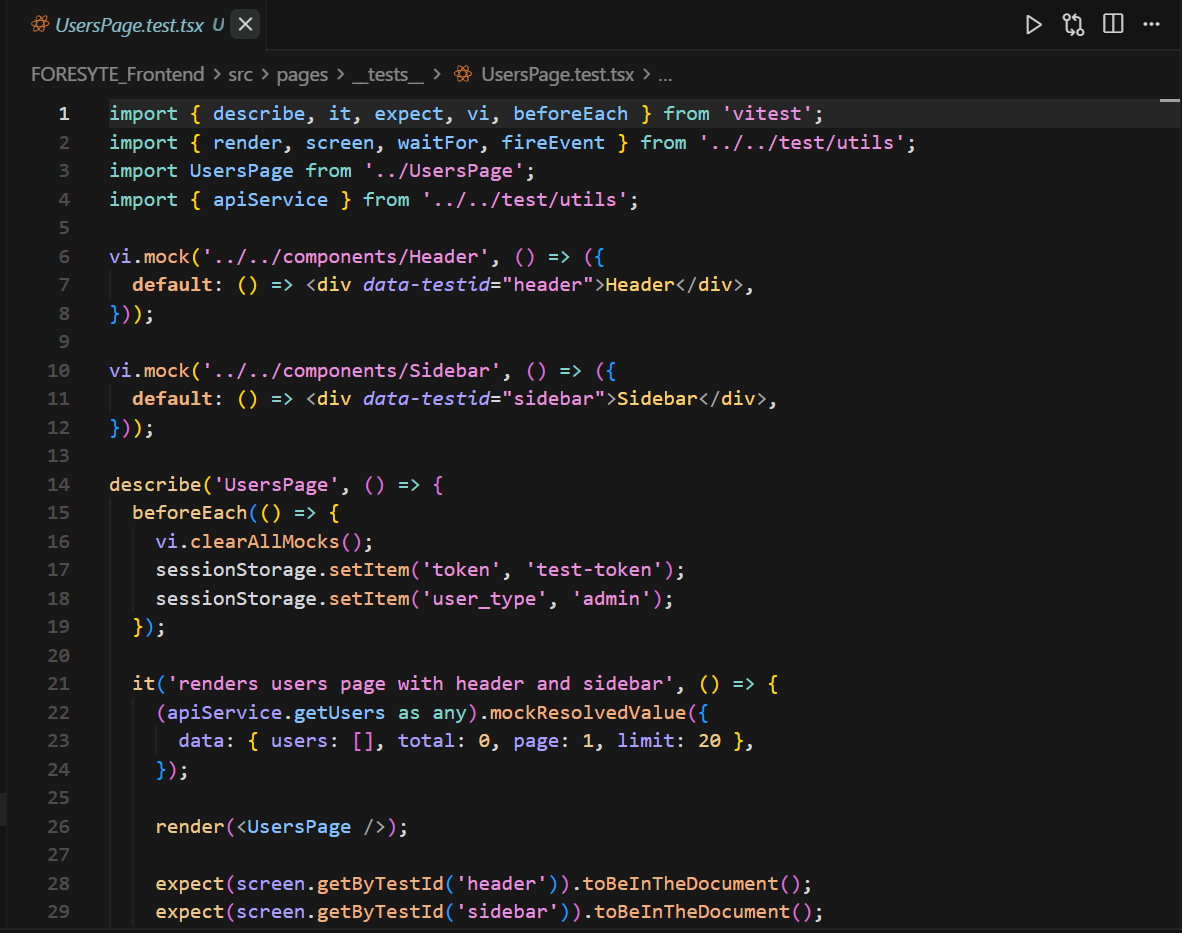
\includegraphics[width=\textwidth]{images/admin/users_page.png}
    \caption{Admin Portal Users Management Page}
    \label{fig:admin-users}
\end{figure}

\subsubsection{Incidents Page}
\begin{figure}[H]
    \centering
    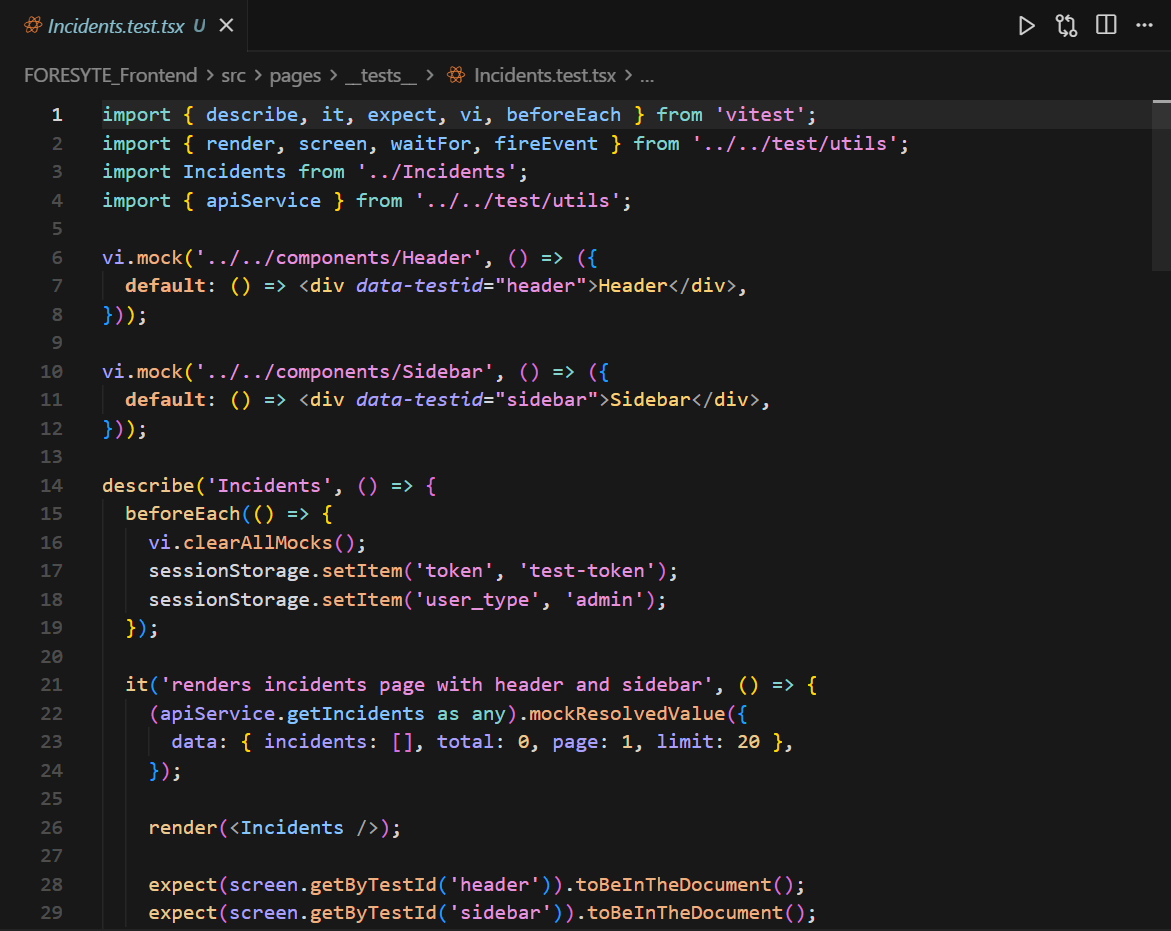
\includegraphics[width=\textwidth]{images/admin/incidents_page.png}
    \caption{Admin Portal Incidents Page}
    \label{fig:admin-incidents}
\end{figure}

\subsubsection{Monitoring Page}
\begin{figure}[H]
    \centering
    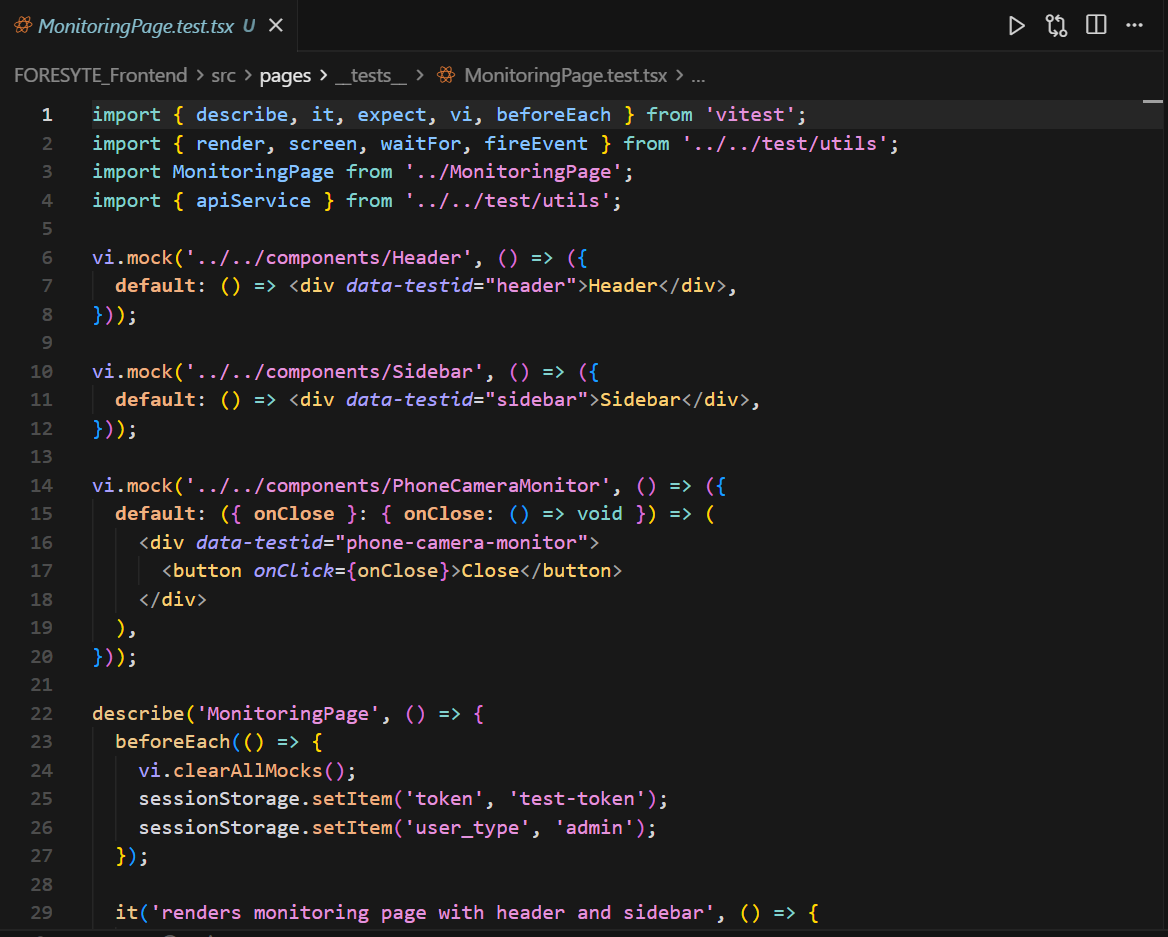
\includegraphics[width=\textwidth]{images/admin/monitoring_page.png}
    \caption{Admin Portal Monitoring Page}
    \label{fig:admin-monitoring}
\end{figure}

\subsubsection{Reports Page}
\begin{figure}[H]
    \centering
    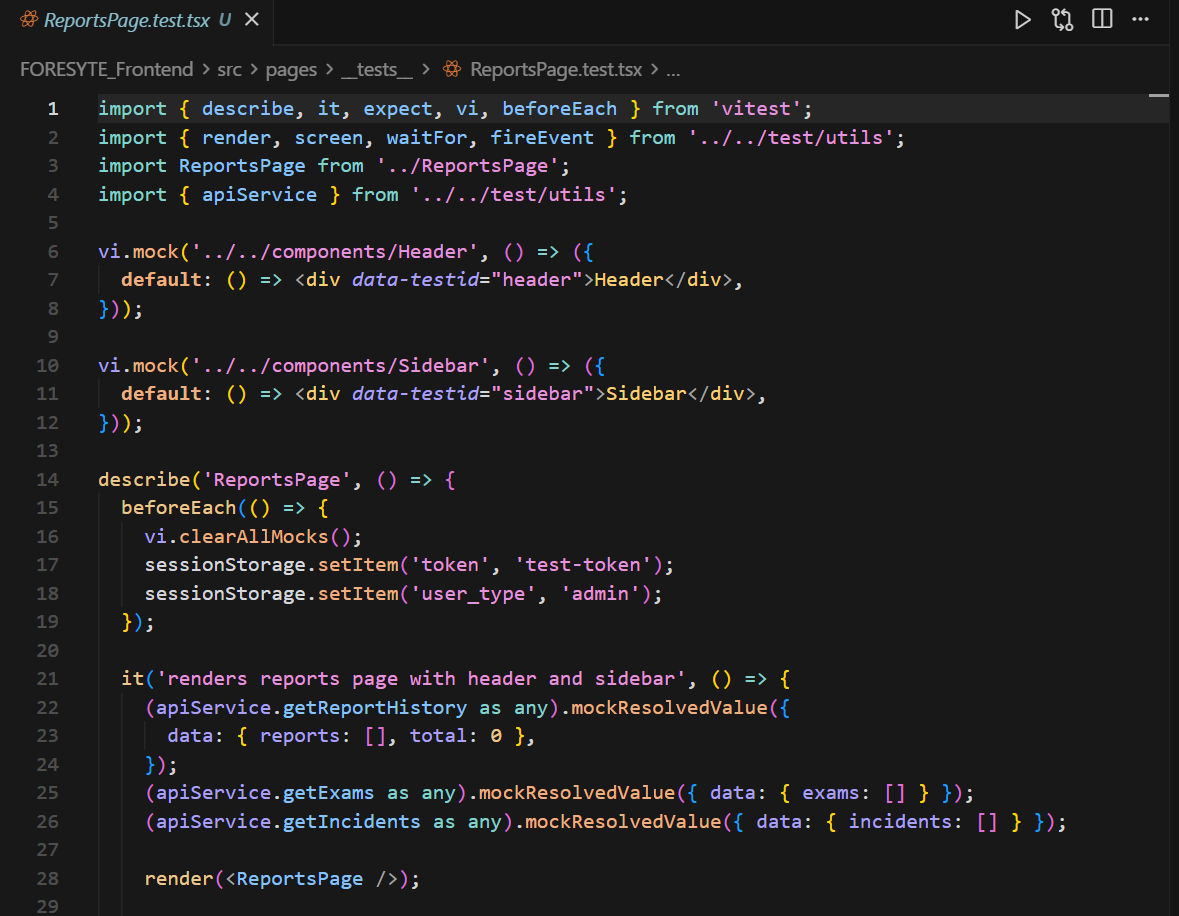
\includegraphics[width=\textwidth]{images/admin/reports_page.png}
    \caption{Admin Portal Reports Page}
    \label{fig:admin-reports}
\end{figure}

\subsubsection{Seating Plan Page}
\begin{figure}[H]
    \centering
    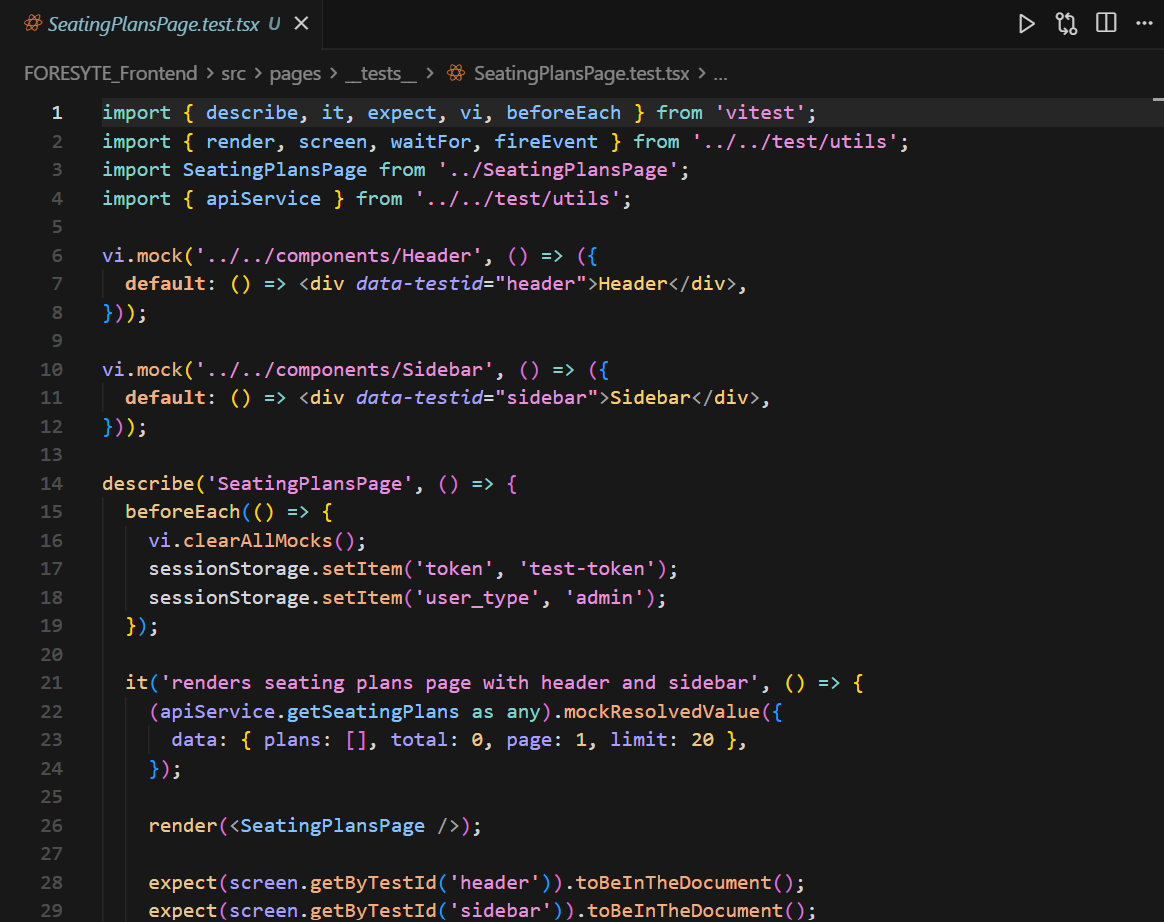
\includegraphics[width=\textwidth]{images/admin/seatingplan_page.png}
    \caption{Admin Portal Seating Plan Management Page}
    \label{fig:admin-seatingplan}
\end{figure}

\subsubsection{Upload Seating Plan Page}
\begin{figure}[H]
    \centering
    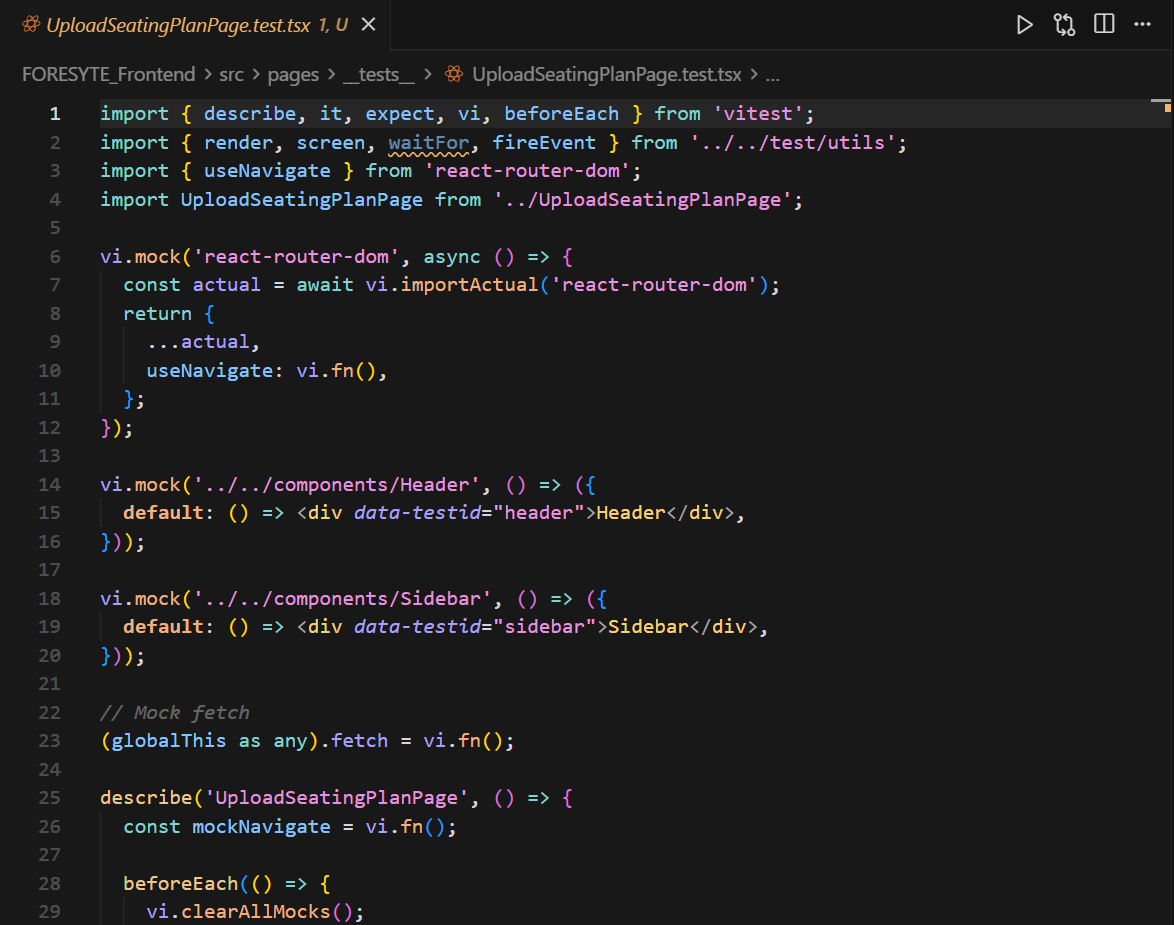
\includegraphics[width=\textwidth]{images/admin/uploadseatingplan_page.png}
    \caption{Admin Portal Upload Seating Plan Page}
    \label{fig:admin-upload-seatingplan}
\end{figure}

\subsubsection{Settings Page}
\begin{figure}[H]
    \centering
    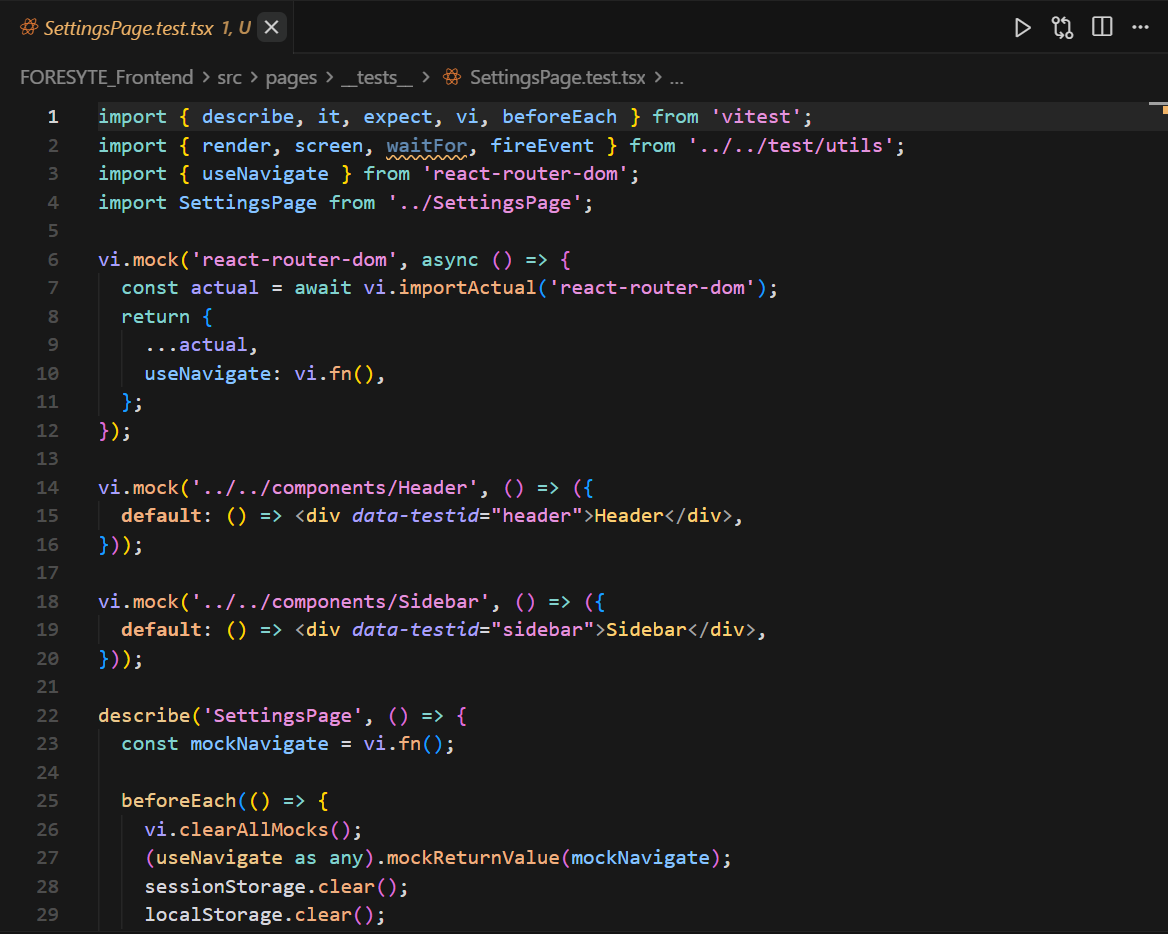
\includegraphics[width=\textwidth]{images/admin/settings_page.png}
    \caption{Admin Portal Settings Page}
    \label{fig:admin-settings}
\end{figure}

\subsubsection{Test Results}
\begin{figure}[H]
    \centering
    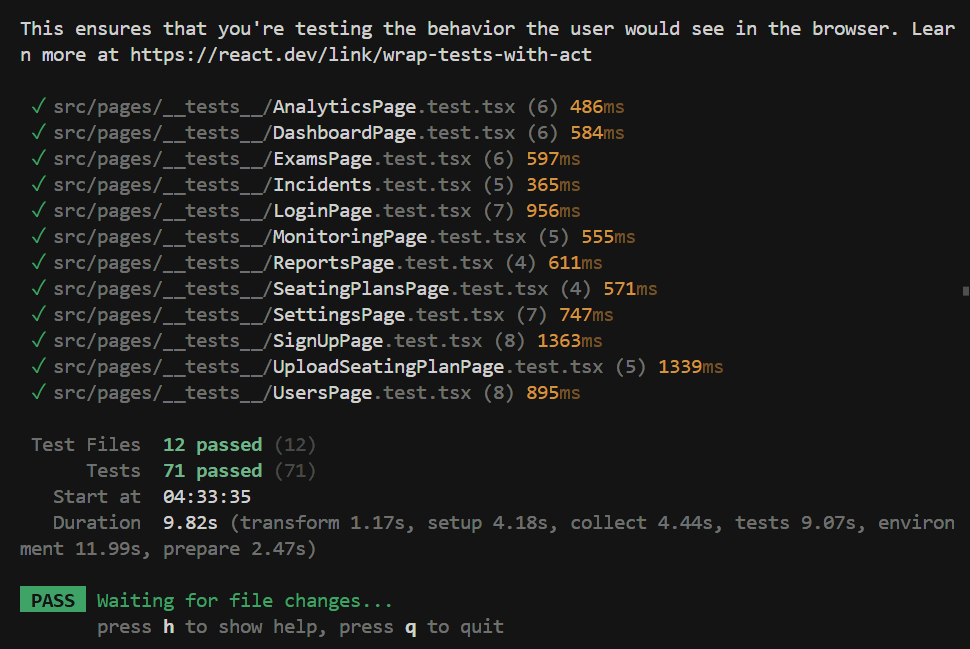
\includegraphics[width=\textwidth]{images/admin/test_results.png}
    \caption{Admin Portal Unit Test Results}
    \label{fig:admin-test-results}
\end{figure}

% ----------------------------------------------------
% INVESTIGATOR
% ----------------------------------------------------

\subsection{Investigator Portal Screenshots}

\subsubsection{Investigator Dashboard}
\begin{figure}[H]
    \centering
    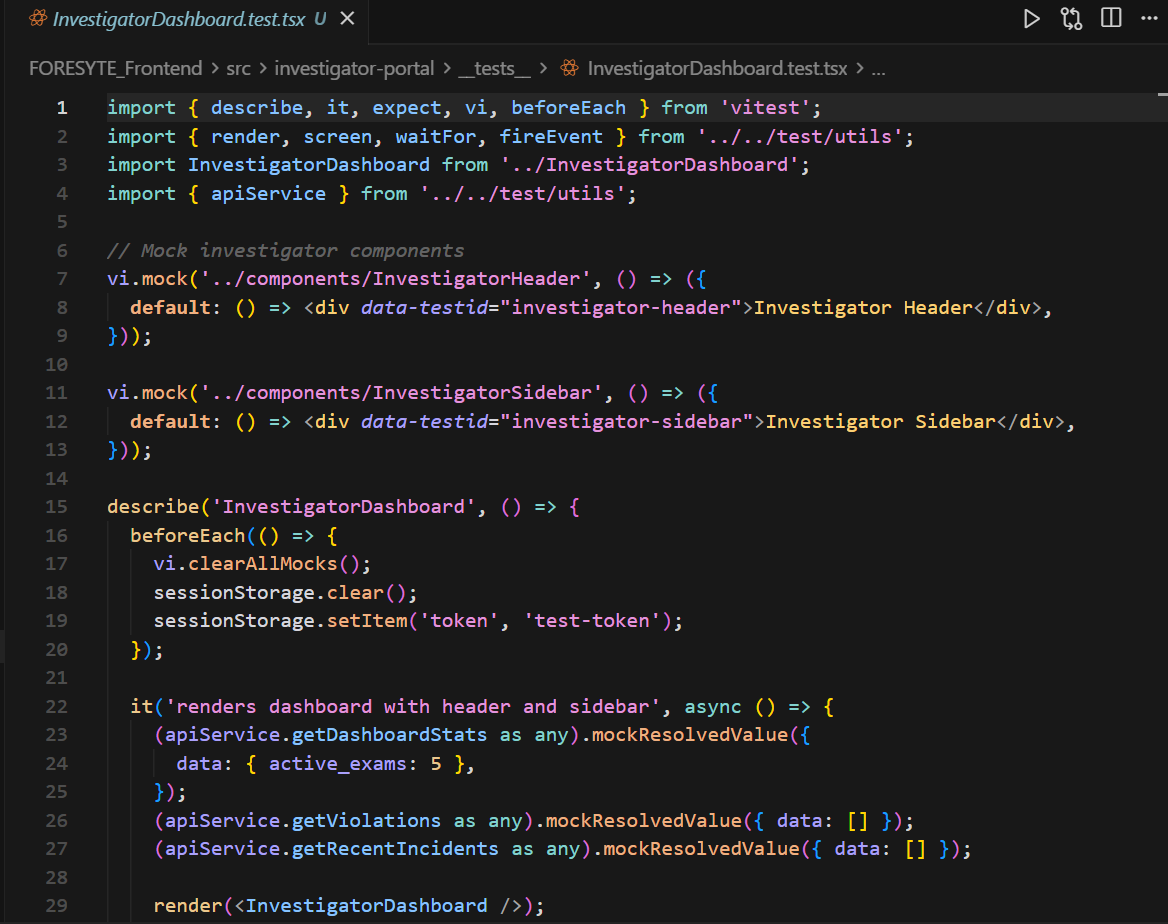
\includegraphics[width=\textwidth]{images/investigator/investigatordashboard_page.png}
    \caption{Investigator Portal Dashboard}
    \label{fig:investigator-dashboard}
\end{figure}

\subsubsection{Violations Page}
\begin{figure}[H]
    \centering
    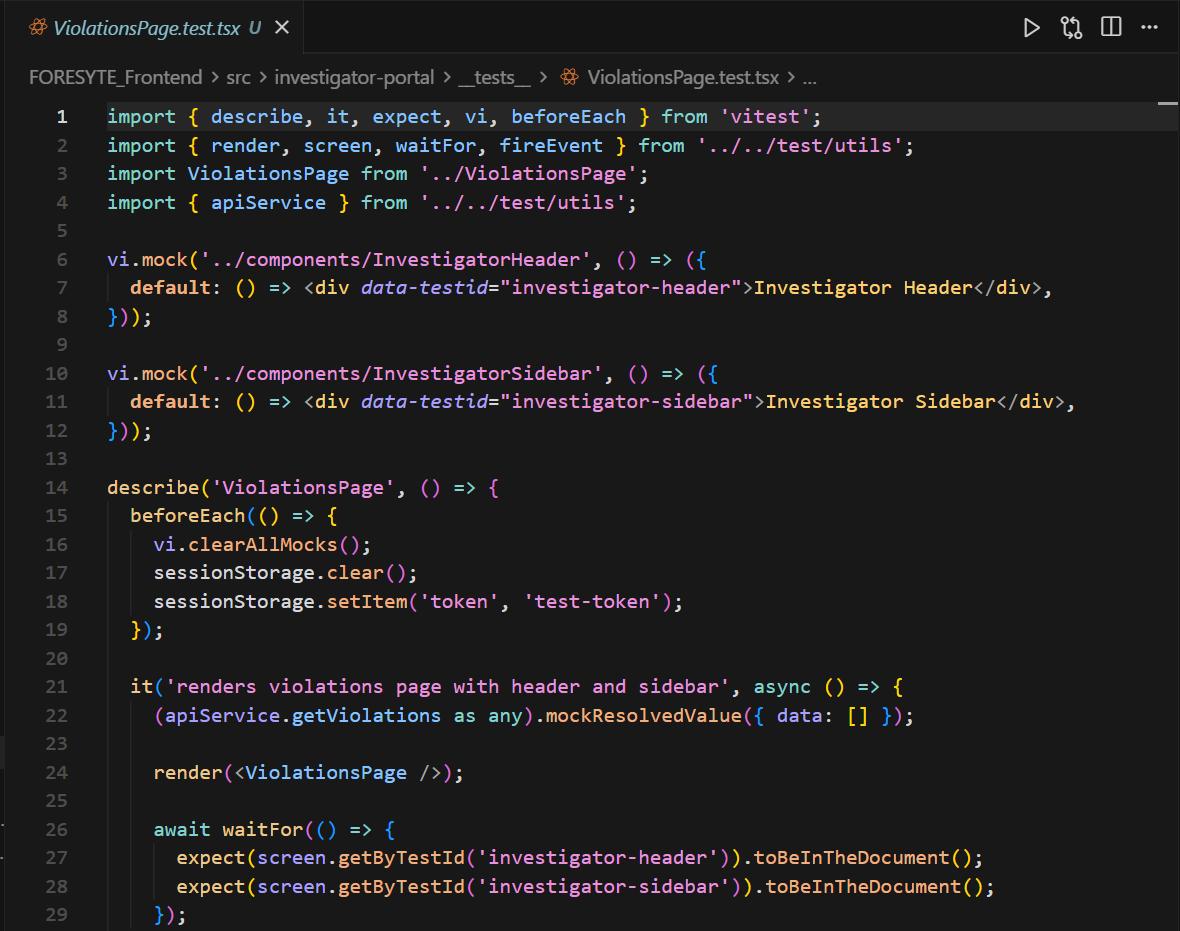
\includegraphics[width=\textwidth]{images/investigator/violations_page.png}
    \caption{Investigator Portal Violations Management Page}
    \label{fig:investigator-violations}
\end{figure}

\subsubsection{Invigilator Activities Page}
\begin{figure}[H]
    \centering
    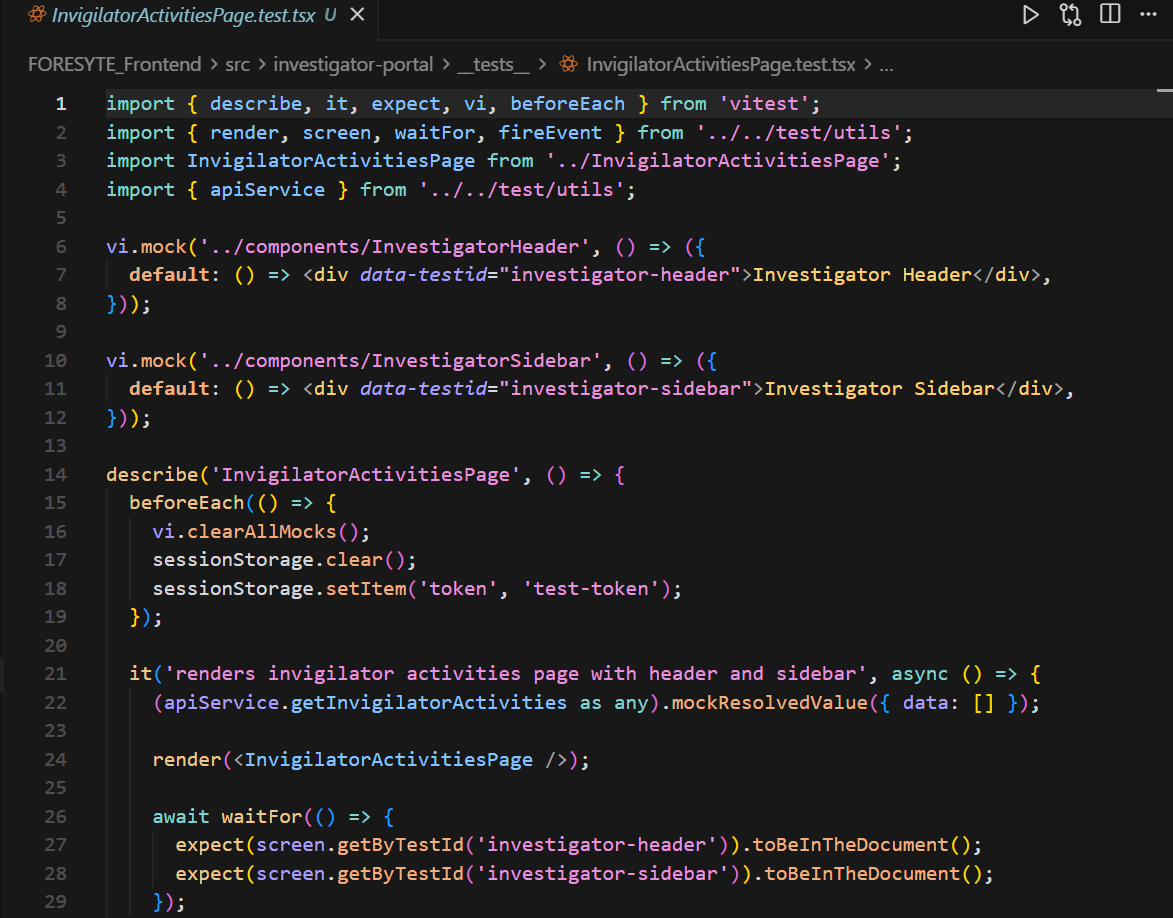
\includegraphics[width=\textwidth]{images/investigator/invigilatoractivities_page.png}
    \caption{Investigator Portal Invigilator Activities Page}
    \label{fig:investigator-invigilator-activities}
\end{figure}

\subsubsection{Student Activities Page}
\begin{figure}[H]
    \centering
    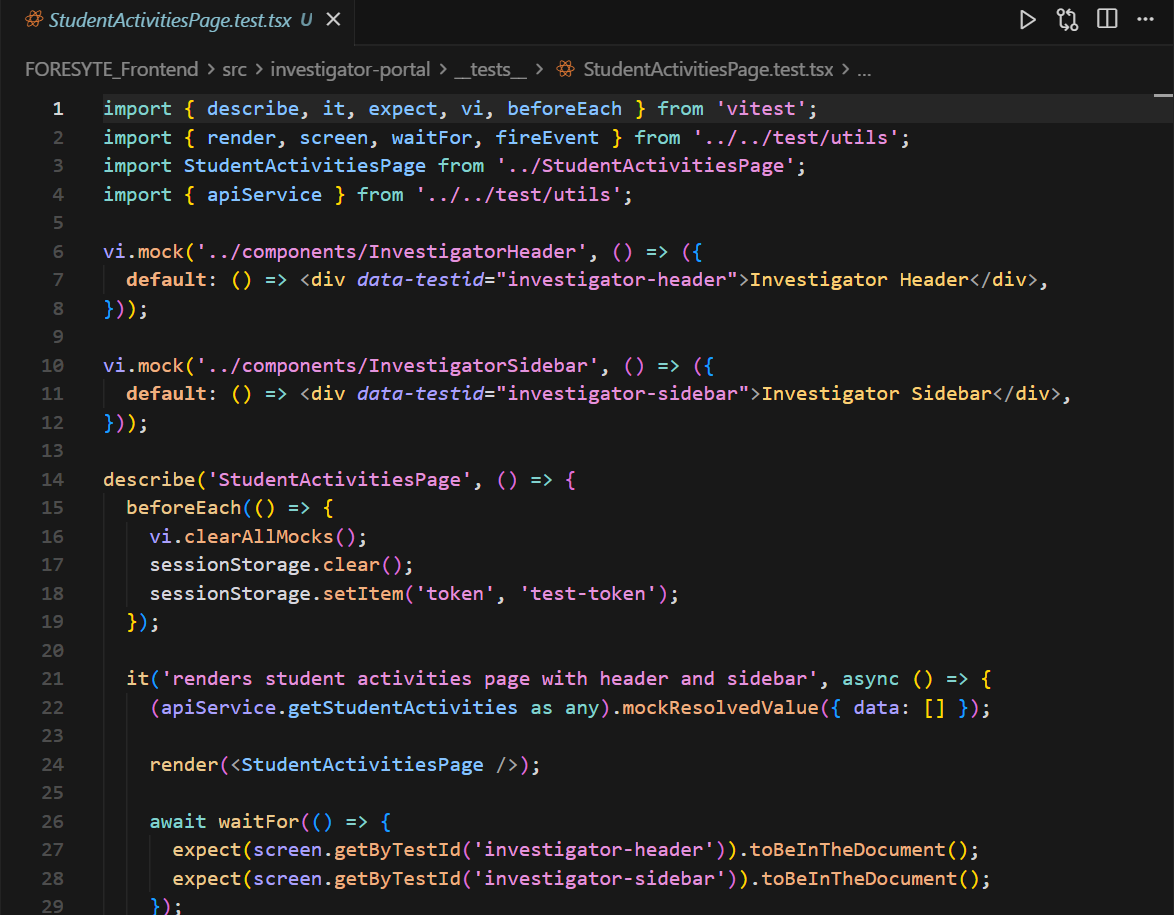
\includegraphics[width=\textwidth]{images/investigator/studentsactivities_page.png}
    \caption{Investigator Portal Student Activities Page}
    \label{fig:investigator-student-activities}
\end{figure}

\subsubsection{Reports Page}
\begin{figure}[H]
    \centering
    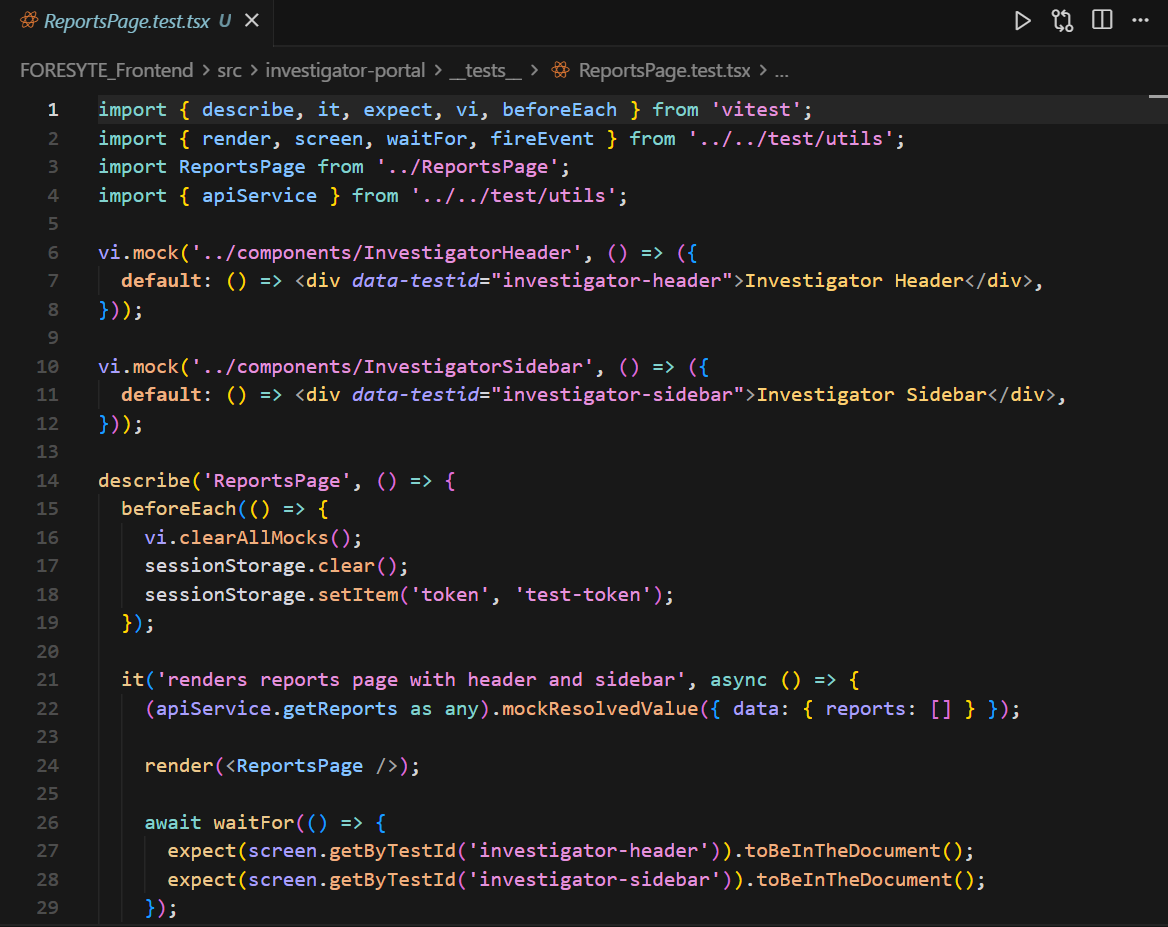
\includegraphics[width=\textwidth]{images/investigator/reports_page.png}
    \caption{Investigator Portal Reports Page}
    \label{fig:investigator-reports}
\end{figure}

\subsubsection{Live Monitoring Page}
\begin{figure}[H]
    \centering
    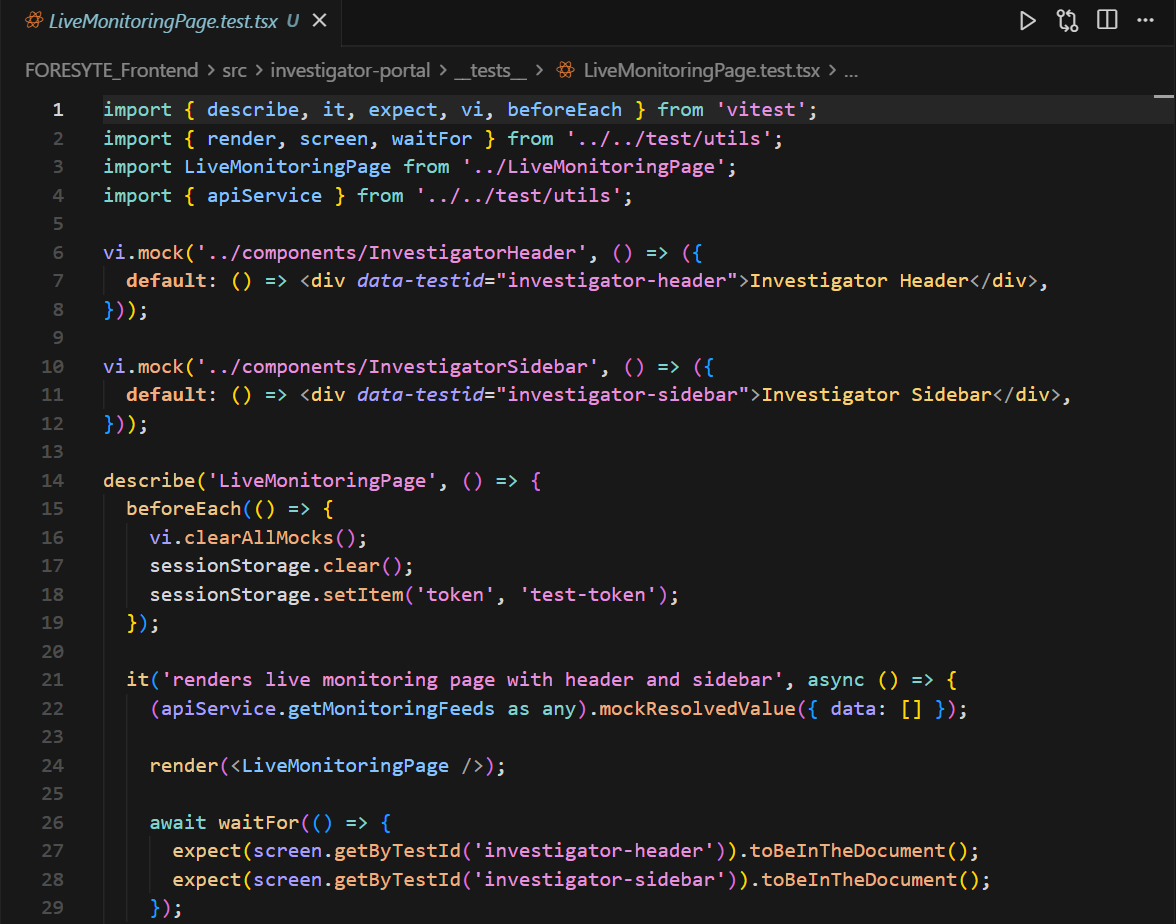
\includegraphics[width=\textwidth]{images/investigator/livemonitoring_page.png}
    \caption{Investigator Portal Live Monitoring Page}
    \label{fig:investigator-live-monitoring}
\end{figure}

\subsubsection{Video Processing Page}
\begin{figure}[H]
    \centering
    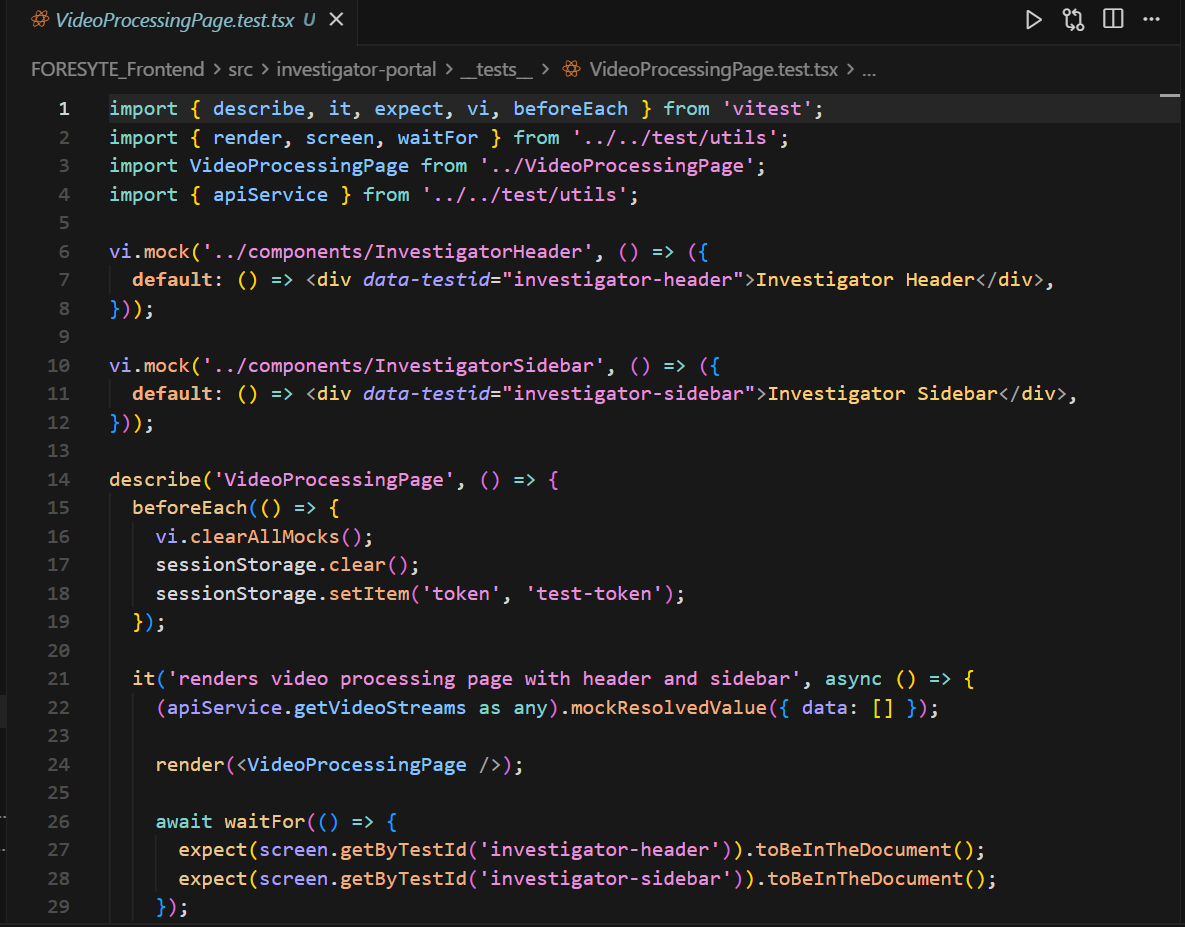
\includegraphics[width=\textwidth]{images/investigator/videoprocessing_page.png}
    \caption{Investigator Portal Video Processing Page}
    \label{fig:investigator-video-processing}
\end{figure}

\subsubsection{Settings Page}
\begin{figure}[H]
    \centering
    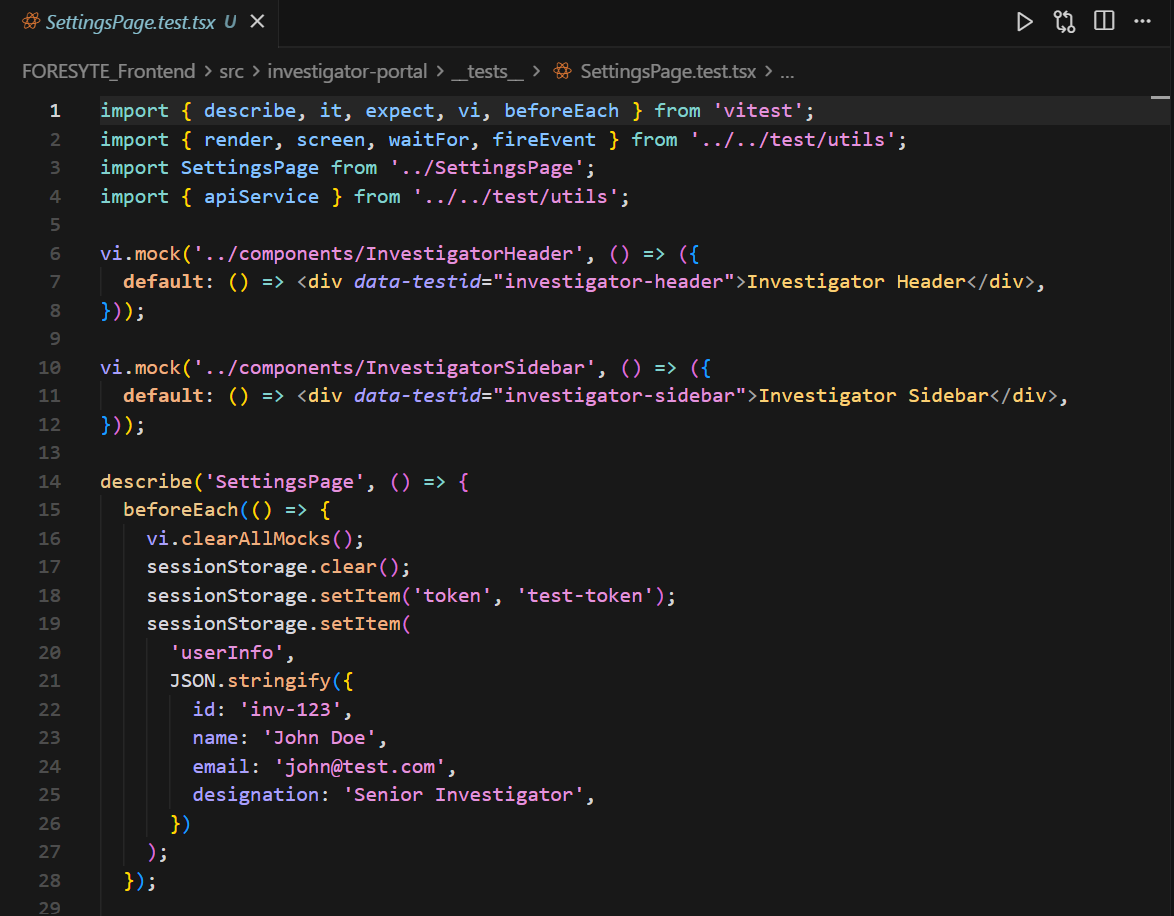
\includegraphics[width=\textwidth]{images/investigator/settings_page.png}
    \caption{Investigator Portal Settings Page}
    \label{fig:investigator-settings}
\end{figure}

\subsubsection{Test Results}
\begin{figure}[H]
    \centering
    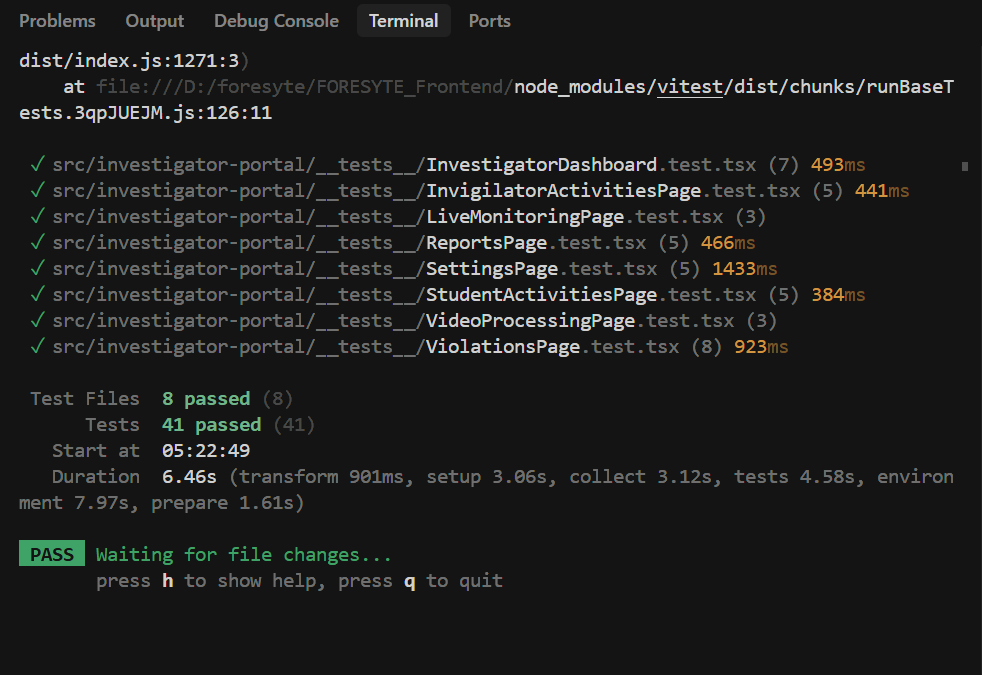
\includegraphics[width=\textwidth]{images/investigator/test_results.png}
    \caption{Investigator Portal Unit Test Results}
    \label{fig:investigator-test-results}
\end{figure}

% ----------------------------------------------------
% STUDENT
% ----------------------------------------------------

\subsection{Student Portal Screenshots}

\subsubsection{Student Dashboard}
\begin{figure}[H]
    \centering
    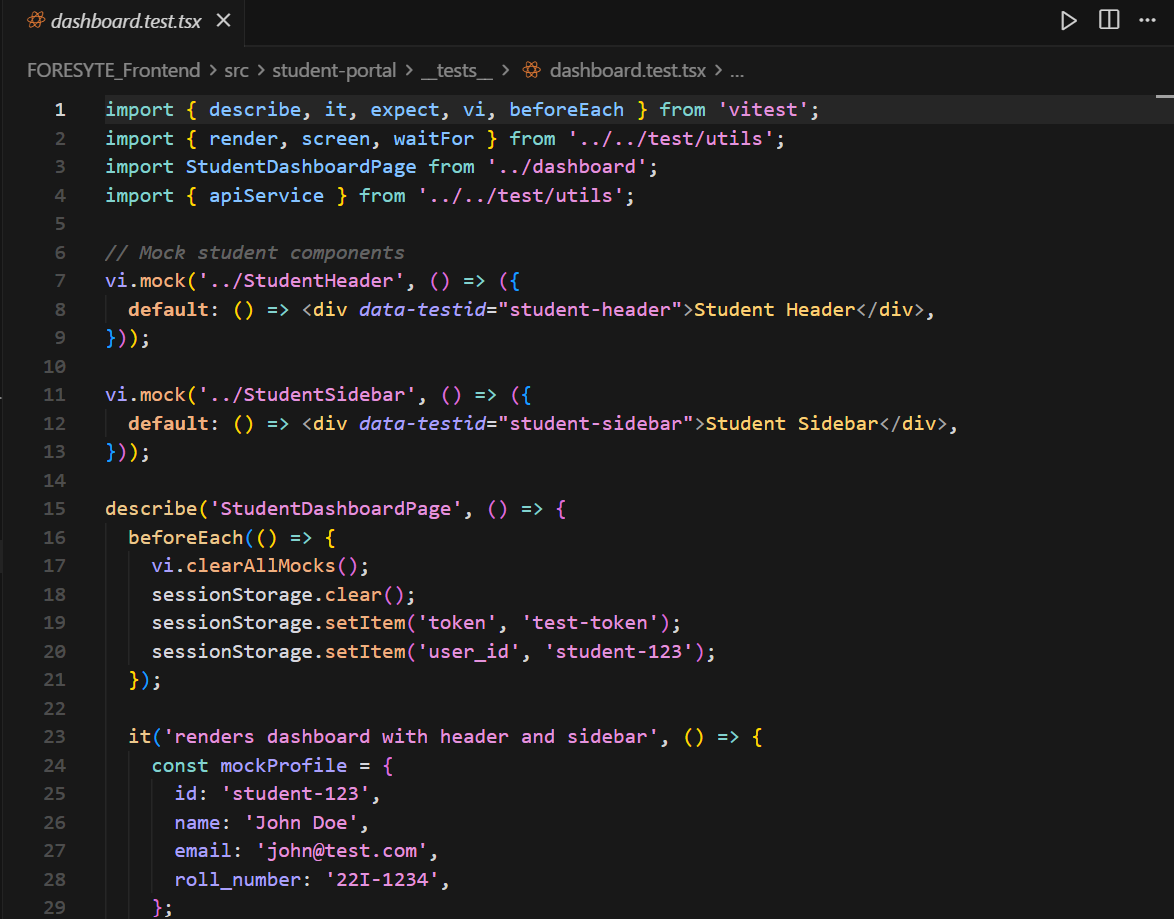
\includegraphics[width=\textwidth]{images/student/dashboard_page.png}
    \caption{Student Portal Dashboard}
    \label{fig:student-dashboard}
\end{figure}

\subsubsection{Disciplinary Records Page}
\begin{figure}[H]
    \centering
    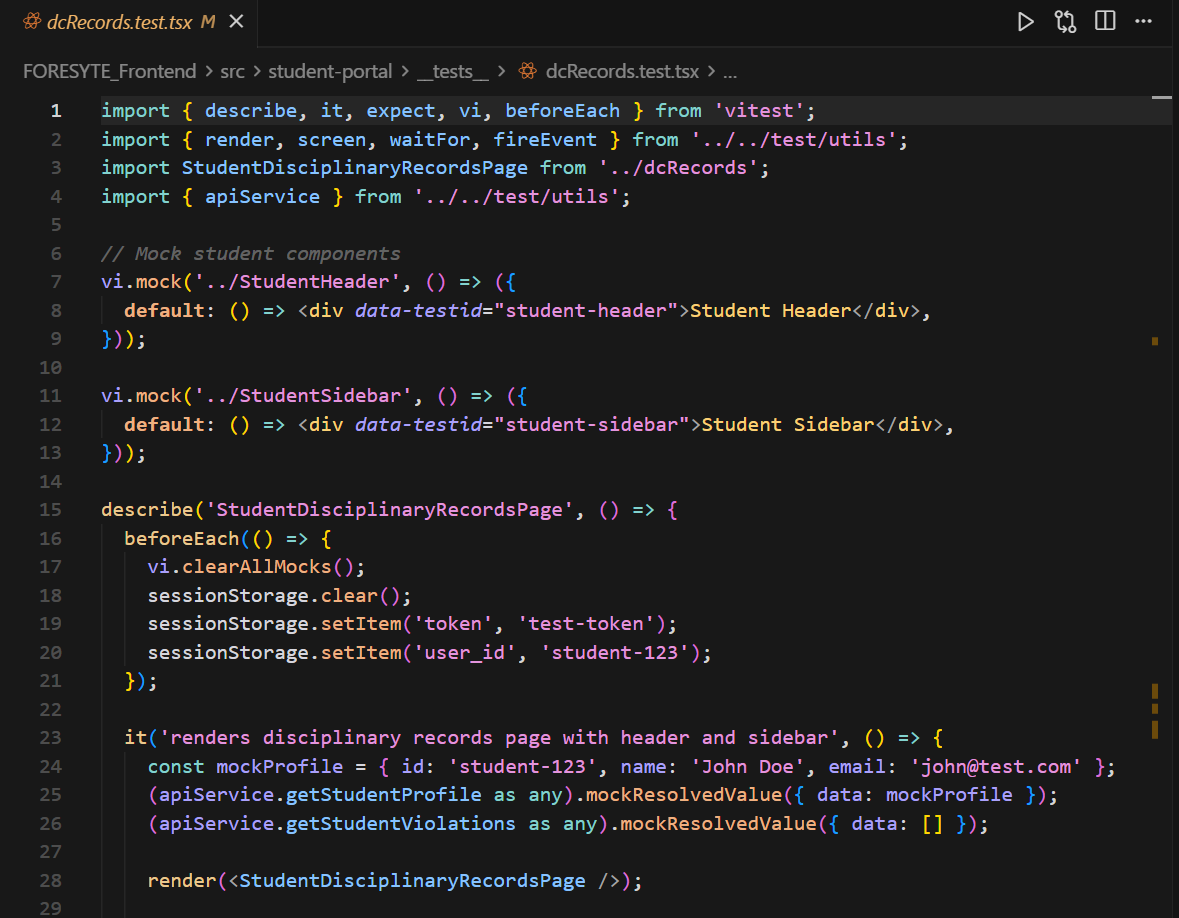
\includegraphics[width=\textwidth]{images/student/dcrecords_page.png}
    \caption{Student Portal Disciplinary Records Page}
    \label{fig:student-dcrecords}
\end{figure}

\subsubsection{Profile Page}
\begin{figure}[H]
    \centering
    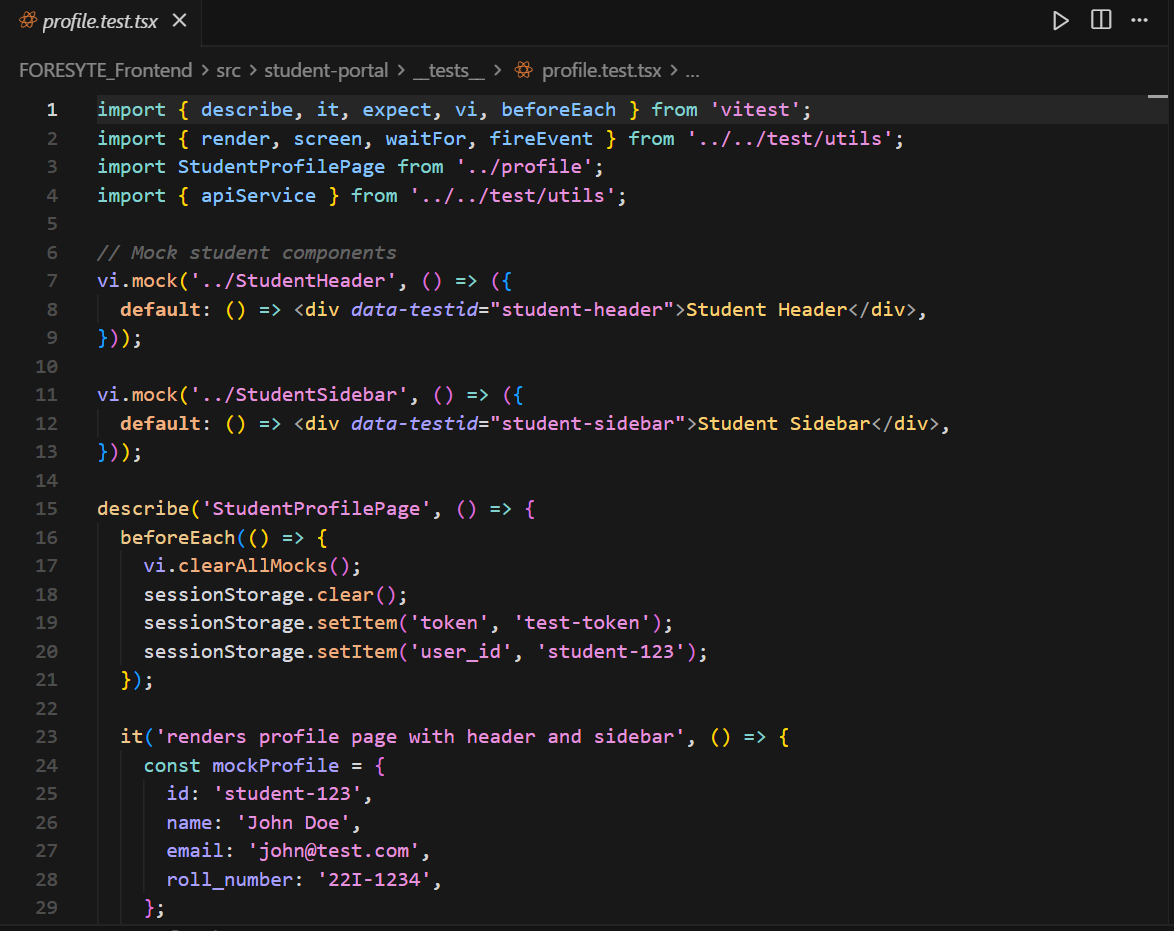
\includegraphics[width=\textwidth]{images/student/profile_page.png}
    \caption{Student Portal Profile Page}
    \label{fig:student-profile}
\end{figure}

\subsubsection{Settings Page}
\begin{figure}[H]
    \centering
    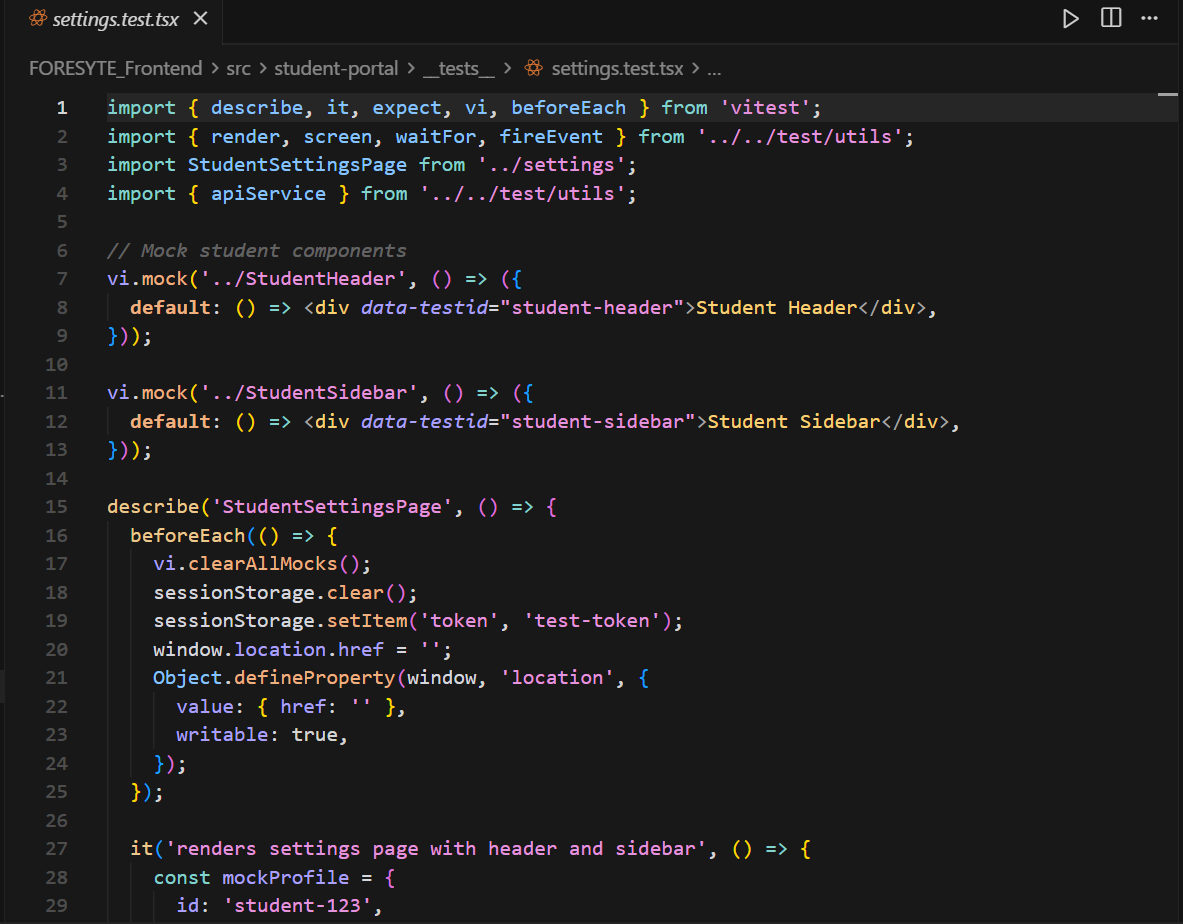
\includegraphics[width=\textwidth]{images/student/settings_page.png}
    \caption{Student Portal Settings Page}
    \label{fig:student-settings}
\end{figure}

\subsubsection{Test Results}
\begin{figure}[H]
    \centering
    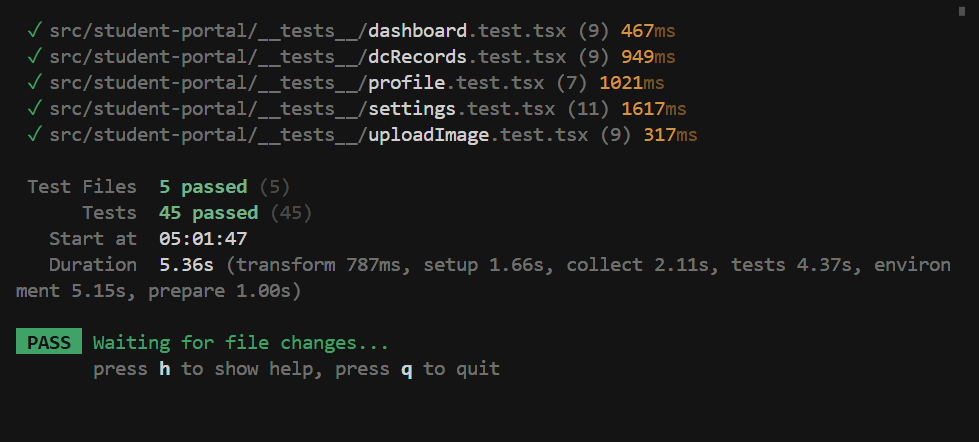
\includegraphics[width=\textwidth]{images/student/test_results.png}
    \caption{Student Portal Unit Test Results}
    \label{fig:student-test-results}
\end{figure}

\end{document}
